\documentclass[12pt,a4paper,openright,twoside]{book}
\usepackage[utf8]{inputenc}
\usepackage{disi-thesis}
\usepackage{code-lstlistings}
\usepackage{notes}
\usepackage{shortcuts}
\usepackage{acronym}
\usepackage{float}

\school{\unibo}
\programme{Corso di Laurea in Ingegneria e Scienze Informatiche}
\title{Eterogeneità dei sistemi di Aggregate Programming: un caso studio con WaveRobot e ThymioRobot}
\author{Elvis Perlika}
\date{\today}
\subject{Objective Oriented Programming}
\supervisor{Chiar.mo Prof. Mirko Viroli}
\cosupervisor{Dott. Gianluca Aguzzi}
\session{III}
\academicyear{2023-2024}

% Definition of acronyms
\acrodef{IoT}{Internet of Thing}
\acrodef{vm}[VM]{Virtual Machine}
\acrodef{JVM}{Java Virtual Machine}
\acrodef{FP}{Functional Programming}
\acrodef{RT}{Referential Transparency}
\acrodef{AP}{Aggregate Programming}
\acrodef{OOP}{Objective Oriented Programming}
\acrodef{AC}{Aggregate Computing}
\acrodef{TDM}{Thymio Device Manager}

\mainlinespacing{1.241} % line spacing in mainmatter, comment to default (1)

\begin{document}

\frontmatter\frontispiece

\begin{abstract}	
    
Il mondo IoT è in costante crescita e di conseguenza nasce la necessità di sviluppare sistemi aggregati, cioè formati da rilevanti quantità di nodi. L'Edge Computing è, ad oggi, l'approccio più utilizzato. Il motivo risiede nel buon compromesso tra capacità computazionale e velocità di comunicazione tra i nodi della rete. Risulta però non in grado di identificare una qualche astrazione di ``Intelligenza Collettiva Emergente'' per via della sua natura fortemente concentra sull'aspetto funzionale dei singoli dispositivi.
La volontà di colmare questa lacuna e quindi di poter creare un'intelligenza distribuita in modo efficace, intuitivo e che permetta di astrarre dalla tecnologia dei dispositivi dell'insieme su cui si vuole definire la strategia operativa ha dato origine al mondo dell'Aggregate Computing. I contesti di applicazione di queste tecnologie sono molteplici, dal controllo di sensori IoT per smart city al controllo di droni in formazione per missioni di salvataggio.
L'obiettivo di questa tesi progettuale è dimostrare come la macroprogrammazione e le tecnologie che ne derivano, come il framework ScaFi e la sua estensione MacroSwarm, risultino essere un paradigma di programmazione particolarmente efficace nella progettazione di sistemi aggregati eterogenei, cioè formati da dispositivi con caratteristiche e protocolli di comunicazione diversi. Si andrà a discute il caso studio dell'integrazione dei robot Thymio in un programma aggregato.

\end{abstract}

\begin{dedication} % this is optional
    Qualsiasi tecnologia sufficientemente avanzata è indistinguibile dalla magia. \\ Terza Legge di Arthur C. Clarke
\end{dedication}

%----------------------------------------------------------------------------------------
\tableofcontents   
\listoffigures     % (optional) comment if empty
\lstlistoflistings % (optional) comment if empty
%----------------------------------------------------------------------------------------

\mainmatter

%----------------------------------------------------------------------------------------
\chapter{Introduzione}
\label{chap:introduction}
%----------------------------------------------------------------------------------------

Negli ultimi anni, il numero di dispositivi interconnessi ha conosciuto una crescita esponenziale, soprattutto nel contesto dell'Internet of Things (IoT). Con un'ampia varietà di dispositivi eterogenei, dalle telecamere di sorveglianza ai sensori industriali, il mondo si sta popolando di sistemi intelligenti capaci di raccogliere, analizzare e scambiare dati in tempo reale. Questa proliferazione porta alla necessità crescente di una tecnologia che possa coordinare il comportamento di gruppi di dispositivi in modo efficace, resiliente e scalabile, soprattutto in contesti dinamici e complessi. In questo scenario, tecniche di controllo collettivo e paradigmi di programmazione aggregata si rivelano fondamentali per garantire che i dispositivi possano operare in sinergia verso obiettivi comuni, gestendo autonomamente le interazioni locali e contribuendo a un comportamento globale emergente. È proprio questo il maggior beneficio della programmazione aggregata, poter creare comportamenti collettivi trascurando gli aspetti comportamentali dei singoli agenti. 
Nel tempo si è compreso che un approccio possibile potesse essere quello di rendere i dispositivi della rete una sorta di ``superorganismo'' in grado di gestirsi autonomamente e che necessiti, eventualmente, solo di comandi ad alto livello dai amministratori del sistema nel caso se ne voglia modificare la strategia. Un esempio di ``superorganismo'' è la \textit{folla} che, pur essendo composta da singoli individui, si muove come un unico organismo che, in certe situazioni, si divide in sottoinsiemi e anche essi si comportano come un unico organismo. 
Per poter far emergere al meglio una intelligenza collettiva anche in sistemi in cui potrebbe non essere immediatamente evidente, è nata la teoria dell'Aggregate Computing. Questa teoria prevede di astrarre dalla tecnologia e dal comportamento dei singoli agenti dell'aggregazione portando l'ambiente reale (o simulato) su cui operano ad essere visualizzato come un campo continuo definito solo dai valori che i singoli agenti restituiscono. La rappresentazione di ogni agente in un valore è detta \textit{calcolo del campo} ed è il nucleo di tale teoria.
Questo lavoro vuole proprio dimostrare come con la possibilità di avere un astrazione totale dalle componenti che andranno a risolvere un certo task in un certo ambiente diventa possibile, con l'avanzare delle tecnologie e delle richieste, integrare nuovi componenti più qualitativi e preformanti senza dover variare la struttura del sistema ma semplicemente integrando, eventualmente, nuove interfacce di comunicazione. Utilizzando le basi definite dal framework ScaFi per la progettazione di programmi aggregati è nato Macroswarm che porta l'intuitività nella costruzione di tali programmi ad un nuovo livello e sarà tale tecnologia ad essere utilizzata nella realizzazione di questo caso studio. 

% //TODO: da finire ?

\paragraph{Struttura della tesi} Nel capitolo \ref{chap:background} approfondimento della lacuna nel settore della progettazione software di larga scala che queste tecnologie vogliono colmare, il linguaggio Scala, i framework per la produzione di Aggregate Program e le tecnologie usate per la realizzazione del caso studio. Nel capitolo \ref{chap:analisi} analisi del problema, obiettivi e requisiti fondamentali per la realizzazione del caso studio. Nel capitolo \ref{chap:design} architettura della infrastruttura per la comunicazione tra i nuovi robot integrati (Thymio) ed il programma aggregato. Nel capitolo \ref{chap:implementazione} sorgenti delle sezioni di codice più rilevanti nello sviluppo del sistema di integrazione del Robot Thymio e test di validazione del sistema aggregato con diversi comportamenti collettivi. In fine nel capitolo \ref{chap:conclusione} conclusioni e sviluppi futuri.

%----------------------------------------------------------------------------------------
\chapter{Background}
\label{chap:background}
%----------------------------------------------------------------------------------------

% I suggest referencing stuff as follows: \cref{fig:random-image} or \Cref{fig:random-image}

% \begin{figure}
%     \centering
%     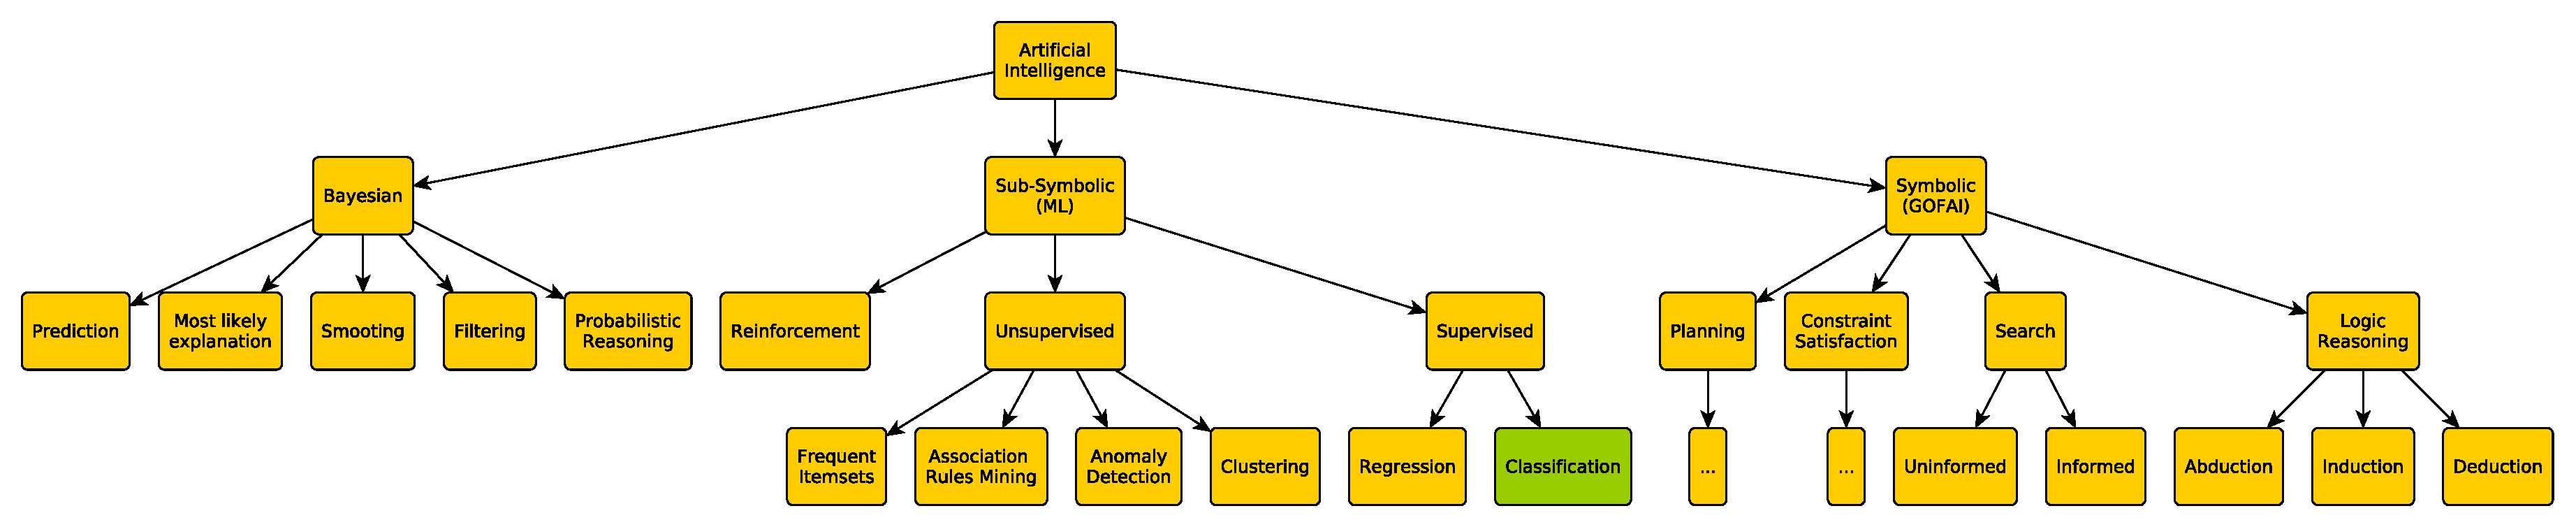
\includegraphics[width=.8\linewidth]{figures/random-image.pdf}
%     \caption{Some random image}
%     \label{fig:random-image}
% \end{figure}

\section{Sistemi collettivi ed eterogenei} 

% Per comprendere il potenziale dell'\ac{AP}, che verrà esplorato nelle sezioni seguenti, è fondamentale definire quale tipo di problema si vuole risolvere. 

La crescita del mondo \ac{IoT} ha portato alla presenza di numerosi dispositivi connessi tra loro. Dispositivi di ogni tipologia e caratterizzati da protocolli di comunicazione eterogenei. Questo settore, in continua evoluzione promette di migliore la produzione, gli spazi di lavoro e la sanità attraverso la raccolta e l'analisi di grandi quantità di dati. È nato, di conseguenza, il bisogno di progettare sistemi resistenti e resilienti con l'obiettivo di gestire queste grandi quantità di dispositivi e dati ed è necessario che questi sistemi siano capaci di: 
\begin{itemize}
    \item adattarsi a cambiamenti imprevedibili: i contesti in cui operano i dispositivi possono cambiare in modo imprevedibile, ad esempio a causa di guasti o malfunzionamenti e prevedere tutti gli scenari risulta essere altamente complesso. 
    \item permettere l'implementazione di nuovi comportamenti: la nascita di nuovi bisogni, variazioni nel ambiente, evoluzione delle tecnologie, ottimizzazione delle risorse o modifiche delle normative richiedono la capacità di implementare nuovi comportamenti in modo rapido ed efficace. 
    \item permettere una capacità di rilevazione e attuazione nel ambiente in modo distribuito e coordinato: la raccolta di informazioni coordinata è cruciale nello sviluppo di un'intelligenza avanzata e la capacità di attuare azioni in modo coordinato è fondamentale per il raggiungimento di obiettivi comuni evitando conflitti e sovrapposizioni. 
\end{itemize}

Allo stato attuale della tecnologia è difficile e costoso progettare sistemi di questo tipo poiché non esistono framework che permettano di gestirne, in modo semplice e intuitivo, la complessità \cite{Beal2015} \cite{CasadeiPhDThesis}.

Un'astrazione grafica del mondo IoT è presente in figura \ref{fig:iot-arc} \cite{Testa2022}. È possibile comprendere come ci sia uno strato contente i nodi (dispositivi)\footnote{HMI: Human-Machine-Interaction.}, uno strato che rappresenta la rete (internet) mediante la quale comunicano\footnote{Prima di accedere alla rete internet le informazioni dei sensori vengono raccolte dai Edge Gateway che si occupano di elaborare ed instradare le informazioni.} ed uno strato contente il mondo Cloud dove vengono raccolte tutte le informazioni prodotte dai nodi della rete e computate, attraverso applicazioni complesse, per l'analisi, la pianificazione, l'ottimizzazione ed altri scopi.

\begin{figure}
    \centering
    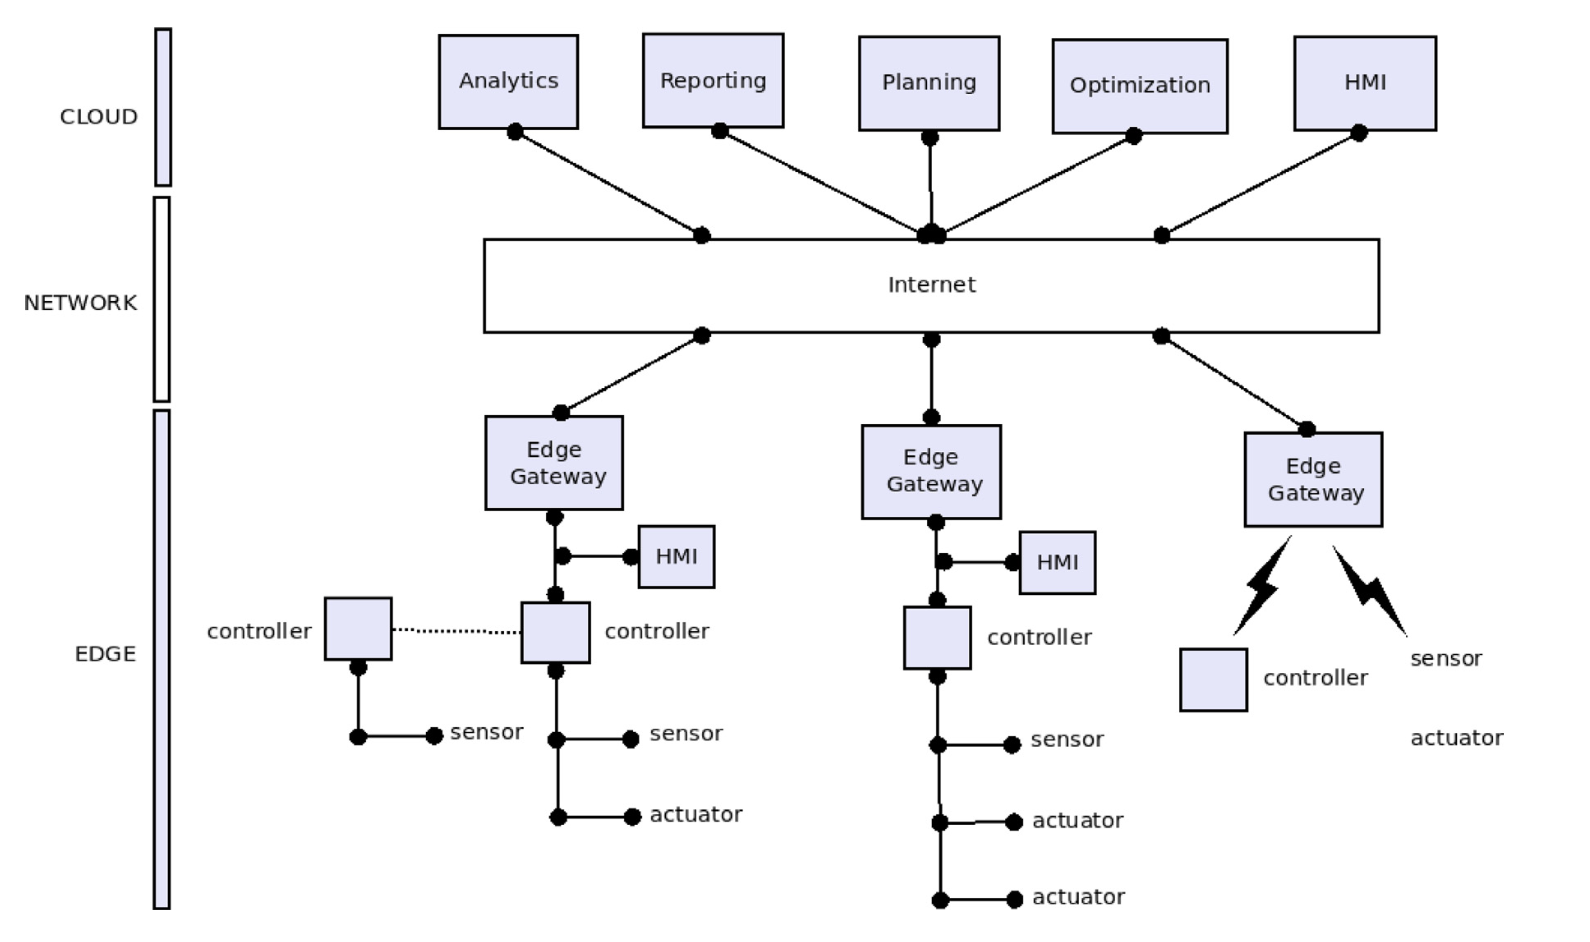
\includegraphics[width=.8\linewidth]{figures/iot-arc.png}
    \caption{Architettura del mondo IoT}
    \label{fig:iot-arc}
\end{figure}

Il problema di questa architettura risiede nell'invio di ingenti quantità di dati da un numero elevato di nodi. Problema che può provocare effetti negativi sui costi, le disponibilità, la scalabilità della piattaforma e la latenza delle comunicazioni. Una delle soluzione trovate è quella di spostare la computazione più vicino possibile ai nodi della rete, in modo da ridurre la quantità di dati da inviare e di conseguenza ridurre i problemi di latenza nelle comunicazioni. Questo approccio, chiamato \textit{Edge Computing} consiste in quattro passaggi principali: 

\begin{enumerate}
    \item raccolta dati
    \item pre-processamento locale dei dati sorgente
    \item definire una strategia immediata 
    \item condivisione della strategia con il Cloud o pre-processamento dei dati sul Cloud
\end{enumerate}

Per quanto semplice, questo approccio va a mettere in una situazione di stress le organizzazioni produttrici di applicazioni e servizi IoT. Inoltre, non è sempre conveniente applicarlo, dipende dal contesto. Ad esempio non sarebbe adatto nel caso i nodi abbiamo specifiche tecniche, come memoria e capacità di calcolo, deboli \cite{Testa2022}. 

Andando ad osservare nel dettaglio solo i dispositivi di questa architettura complessa è possibile notare come molto spesso, anche se in apparenza impercettibile, è presente un aspetto collettivo che merita di essere considerato. Preso un sistema in cui è presente una gestione dei dati distribuita, nella quale i nodi della rete condividono le proprie informazioni e quelle che hanno ricevuto da altri nodi al fine di raggiungere un obiettivo comune, se questo sistema è in grado di adattarsi ai cambiamenti e continuare nella realizzazione del task è possibile che esso vada a far emergere una forma di intelligenza collettiva autonoma. 

La forza di un sistema del genere sta nella sua resilienza: ogni nodo può operare localmente con regole relativamente semplici, ma la somma delle interazioni può produrre una risposta globale complessa e adattabile. Tale struttura è particolarmente efficace in contesti in cui è richiesta una risposta flessibile e continua agli imprevisti, come nei casi di reti neurali distribuite, sistemi di swarm robotics, e ambienti IoT (Internet of Things) su larga scala.

Questa intelligenza distribuita può, quindi, essere considerata autonoma nella misura in cui non richiede una gestione decentralizzata per adattarsi o evolversi, riuscendo a creare soluzioni nuove senza un controllo diretto. Questo fenomeno diventa particolarmente evidente in situazioni di problem-solving distribuito, dove i nodi, seguendo semplici protocolli di comunicazione e scambio, ottimizzano il risultato collettivo e provocando un miglioramento delle capacità del sistema nel raggiungere gli obiettivi prefissati.

Sono numerosi i casi di sistemi collettivi che necessitano di un controllo distribuito e coordinato. Un esempio pratico di questa intelligenza collettiva autonoma si può vedere nelle reti di sensori distribuiti, che monitorano in tempo reale fenomeni ambientali (come incendi, movimenti sismici o cambiamenti climatici). Ogni sensore condivide dati con quelli vicini e l'intero sistema è in grado di rilevare e rispondere ad anomalie senza un controllo centrale. Un altro esempio è il controllo di droni in formazione, in questo caso, ogni drone deve essere in grado di comunicare con i propri vicini per mantenere la formazione, evitare collisioni e raggiungere l'obiettivo comune come in figura \ref{fig:drones}.

È chiara la necessità di una tecnologia che permetta di costruire nuove applicazioni (o comportamenti) per il controllo di collettivi di dispositivi senza dover andare a definire i singoli comportamenti dei dispositivi, bensì trattando l'unione di questi singoli dispositivi come un unico superorganismo.

\begin{figure}
    \centering
    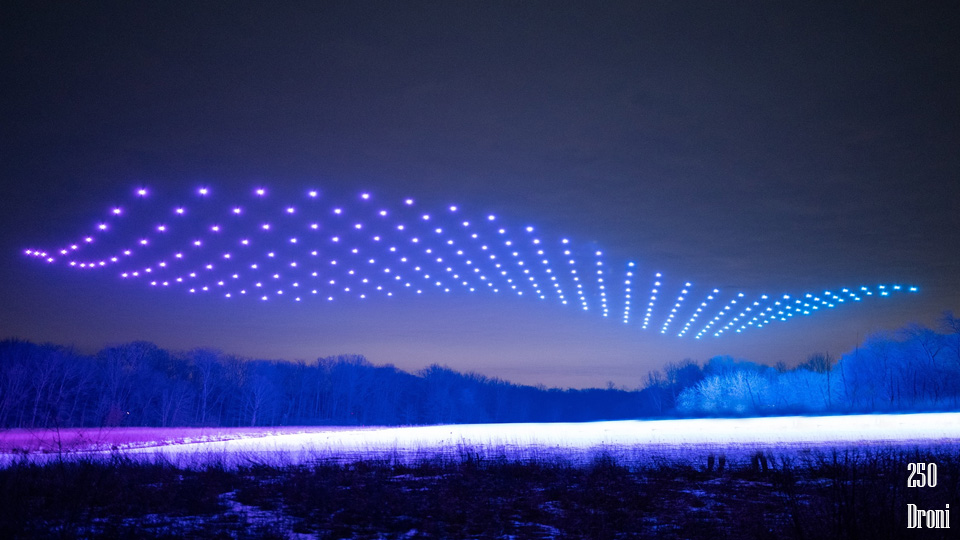
\includegraphics[width=.7\linewidth]{figures/drones.jpg}
    \caption{Droni in formazione in ambiente notturno}
    \label{fig:drones}
\end{figure}

\section{Scala}

Per la realizzazione del progetto di questa tesi si è scelto di utilizzare il linguaggio di programmazione Scala. Per comprenderlo meglio è necessario fare una breve introduzione alla programmazione funzionale.

È possibile riassumere il paradigma della programmazione funzionale con la frase \textit{``Everything is a Function''}. Quando si parla di funzioni in quest'ambito si fa riferimento alle \textbf{funzioni pure}\cite{Hunt2018}, cioè funzioni ``prive di effetti collaterali''. Con l'espressione ``priva di effetti collaterali'' si intende una funzione che non fa altro oltre a restituire un risultato (come la modifica del campo di un oggetto o la scrittura/lettura su file).

\label{sec:fp}
Nel dettaglio, per \textbf{funzione pura} si intende una funzione $f:A\to B$, (una funzione che prende un input di tipo $A$ e restituisce un output di tipo $B$) che mette in relazione ogni elemento di $A$ con esattamente un valore di $B$. Qualsiasi altra operazione che non sia utile a calcolare $f(a)=b$ con $a\in A$ e $b\in B$ deve essere intesa come effetto collaterale della funzione e quindi evitata se si vuole creare una funzione pura.

Un esempio di funzione pura, senza effetti collaterali, è la funzione di somma che prende in input due valori e ne restituisce la loro somma. 

Si potrebbe pensare che con l'uso della \ac{FP} si possano costruire solo programmi semplice, nella realtà non c'é alcuna limitazione sulla complessità del software da costruire poiché questo paradigma non rappresenta reali estensioni strutturali al paradigma \ac{OOP}, bensì esprime un nuovo modo di pensare e scrivere il codice. È possibile immaginare tale paradigma come una filosofia nel mondo della programmazione.

In oltre, la programmazione funzionale incoraggia l'uso di dati immutabili, il che significa che una volta creato un dato, non viene modificato. Questo riduce le possibilità di errori difficili da tracciare, perché le funzioni non alterano lo stato globale ma restituiscono nuovi valori. Nei progetti complessi, ciò rende più facile comprendere e prevedere il comportamento del codice.  Grazie all'immutabilità e alle funzioni pure, la programmazione funzionale è particolarmente adatta per il calcolo parallelo e concorrente. L'assenza di modifiche condivise tra le funzioni evita il problema dei \textit{race condition}, che si verifica quando due processi cercano di accedere o modificare contemporaneamente lo stesso dato. Questo è cruciale per la scalabilità nei sistemi complessi.

Queste proprietà rendono i programmi facili da testare e da correggere nel caso di bug. Di conseguenza rendono un programma progettato con approccio funzionale maggiormente scalabile e mantenibile.

Scala è un linguaggio Java-like moderno e flessibile progettato per unificare il paradigma \ac{OOP} e quello \ac{FP}.  È stato creato da \textbf{Martin Odersky} ed è molto utilizzato per applicazioni di tipo Big Data, elaborazione distribuita e backend.

Caratteristiche principali di Scala:
\begin{itemize}
    \item Orientato agli oggetti: Significa che ogni valore è un oggetto. Supporta classi, oggetti, eredità e polimorfismo come in Java.
    \item Funzionale: Scala integra concetti di programmazione funzionale, come funzioni pure, immutabilità, e supporta anche higher-order functions (funzioni che accettano altre funzioni come argomenti o che ritornano funzioni). Le funzioni sono trattate come “valori di prima classe,” ovvero possono essere passate e manipolate come dati.
    \item Sintassi concisa: Scala è progettato per ridurre il codice \textit{boilerplate} (codice ridondante) presente in linguaggi come Java. Ad esempio, la gestione dei getter e setter delle proprietà viene automatizzata grazie alle case classes e alla sintassi compatta di Scala.
    \item Tipi statici avanzati: Scala ha un sistema di tipi statici potente e flessibile, che permette di rilevare molti errori a tempo di compilazione. Supporta tipi generici, tipi astratti e altre funzionalità avanzate, come i traits (simili alle interfacce in Java, ma con possibilità di implementare metodi).
    \item Compatibilità con Java: Scala è completamente compatibile con Java. Può usare qualsiasi libreria Java, il che lo rende ideale per progetti che devono integrarsi con applicazioni Java esistenti o fare uso dell'ecosistema Java.
\end{itemize}

L'utilizzo della \ac{JVM} e la flessibilità del linguaggio sono state le caratteristiche chiave per il raggiungimento della popolarità di questo linguaggio.

Non è, però, privo di difetti:

\begin{itemize}
    \item Curva di apprendimento ripida: La combinazione di OOP e FP può essere complessa da apprendere per chi è abituato a linguaggi puramente orientati agli oggetti.
    \item Tempi di compilazione più lunghi: Scala può avere tempi di compilazione più lenti rispetto a Java, specialmente per progetti molto grandi.
\end{itemize}

\begin{quote}
    \centering
    Quindi perché usare Scala?
\end{quote}

Il motivo per cui Scala è un linguaggio particolarmente adatto per la programmazione di sistemi di \ac{AC} è dovuto proprio alla sua flessibilità, essa permette di lavorare sui campi di calcolo, che necessitano di essere supportati dalle seguenti proprietà, in modo molto naturale:

\begin{itemize}
    \item una sintassi coincisa per definire funzioni sui campi, le quali in Scala sono le espressioni standard
    \item meccanismi di controllo sul \textit{quando} e \textit{come} le espressioni vengono valutate
    \item capacità di calcolare lo stato di un campo basandosi sulle informazioni più recenti dei nodi presenti nel suo intorno
\end{itemize}

In Scala ogni valore è un oggetto ed i comportamenti vengono definiti attraverso i metodi. Per implementare un campo di calcolo in Scala andremo a definire gli operato dei campi attraverso la definizione di metodi che verranno interpretati dagli oggetti sui quali sono stati chiamati. Gli oggetti, in questo modo, possono essere visti come macchine virtuali in locale per l'esecuzione degli operatori di campo.

\section{Stato dell'arte}

L'Aggregate Programming è un concetto che nasce dal paradigma della ``macro programmazione''.

Con \textit{paradigma di macro-programmazione} si intende la teoria (e la pratica) per la progettazione di singoli programmi che gestiscono il controllo di ``macro'' comportamenti, cioè comportamenti di collettivi di componenti. La definizione data in letteratura è  la seguente:

\begin{quote}
    Paradigma astratto per programmare il comportamento (macro) scopico di sistemi formati da entità computazionali. \cite{Casadei2023}
\end{quote}

Questo paradigma nasce con lo scopo di astrarre il comportamento e le interazioni tra i singoli componenti del sistema e si basa su quattro principi fondamentali \cite{Casadei2023}:

\begin{itemize}
    \item \textit{Distinzione micro-macro.} Per \textit{micro} si intendono le singole entità del ambiente, mentre per \textit{macro} si intende il comportamento del sistema, il suo stato, la sua struttura.
    \item \textit{Prospettiva macroscopica.} Il programmatore si concentra principalmente sul comportamento macroscopico del sistema, piuttosto che sul comportamento dei singoli componenti, questo non esclude osservazioni a livello microscopico.
    \item \textit{Macro-programma.} L'attività di sviluppo genera un ``macroprogramma'', ovvero un codice che specifica la logica di funzionamento macroscopica (globale).
    \item \textit{Mappatura macro a micro.} Anche conosciuta come \textit{mappatura globale a locale}, è la logica che permette al macro-programma di compiere le specifiche attuazioni a livello microscopico per completare il task.
\end{itemize}

Questa teoria e la tecnologia che ne deriva mira a migliorare la progettazione, manutenzione e testing di programmi nell'ambito del controllo di dispositivi hardware di larga-scala. 

L'Aggregate Computing (AC) si basa sulla mappatura di un mondo cyber-fisico in un nuovo modello logico. Da un punto di vista strutturale un sistema \textbf{aggregato} è una rete di dispositivi, capaci di computare, equipaggiati con (o sui quali è possibile equipaggiare) sensori ed attuatori. Ogni dispositivo corrisponde ad un nodo e questi nodi sono connessi tra di loro secondo una logica di vicinato che può essere definita in base alla distanza fisica o alla comunicazione. Da un punto di vista comportamentale, invece, ogni nodo interpreta il programma aggregato solo in relazione al proprio contesto locale. Da un punto di vista delle interazioni, i nodi estraggono informazione dal proprio vicinato e propagano le proprie nello stesso contesto. Queste interazioni son ciò che permettono al contesto locale e globale di influenzarsi reciprocamente.

La tecnica dell'Aggregate Computing si basa su tre principi fondamentali per la costruzione di sistemi robusti e resilienti:

\begin{itemize}
    \item \textbf{Aspetto strutturale.} I dettagli implementativi dei sistemi hardware che si vuole andare a manipolare devono essere nascosti così da permettere ai programmatori di concentrarsi solo sulla logica di alto livello del sistema. In alcuni casi è possibile che questa astrazione delle specifiche di basso livello sia tale da poter pensare al dominio come uno spazio continuo, invece di un insieme di dispositivi separati. Per esempio, invece di immaginarci una stanza piena di sensori, la trattiamo come una area unificata definita da un flusso continuo di dati (figura \ref{fig:points-to-linear}).
    \item \textbf{Aspetto comportamentale.} Il programma manipola le strutture dati della rete di dispositivi sia in funzione della loro estensione spaziale che di quella temporale. Approccio particolarmente utile in sistemi in cui l'informazione cambia in base al luogo (figura \ref{fig:different-function}).
    \item \textbf{Aspetto interazionale.} Ogni dispositivo della rete esegue le operazioni necessarie in autonomia, coordinandosi con i dispositivi vicini attraverso meccanismi robusti e resilienti. In questo modo il sistema rimane fluido ed efficiente anche in situazioni anomale, ad esempio causate dal guasto di un qualche dispositivo (figura \ref{fig:lost-nodes}).
\end{itemize}

\begin{figure}
    \centering
    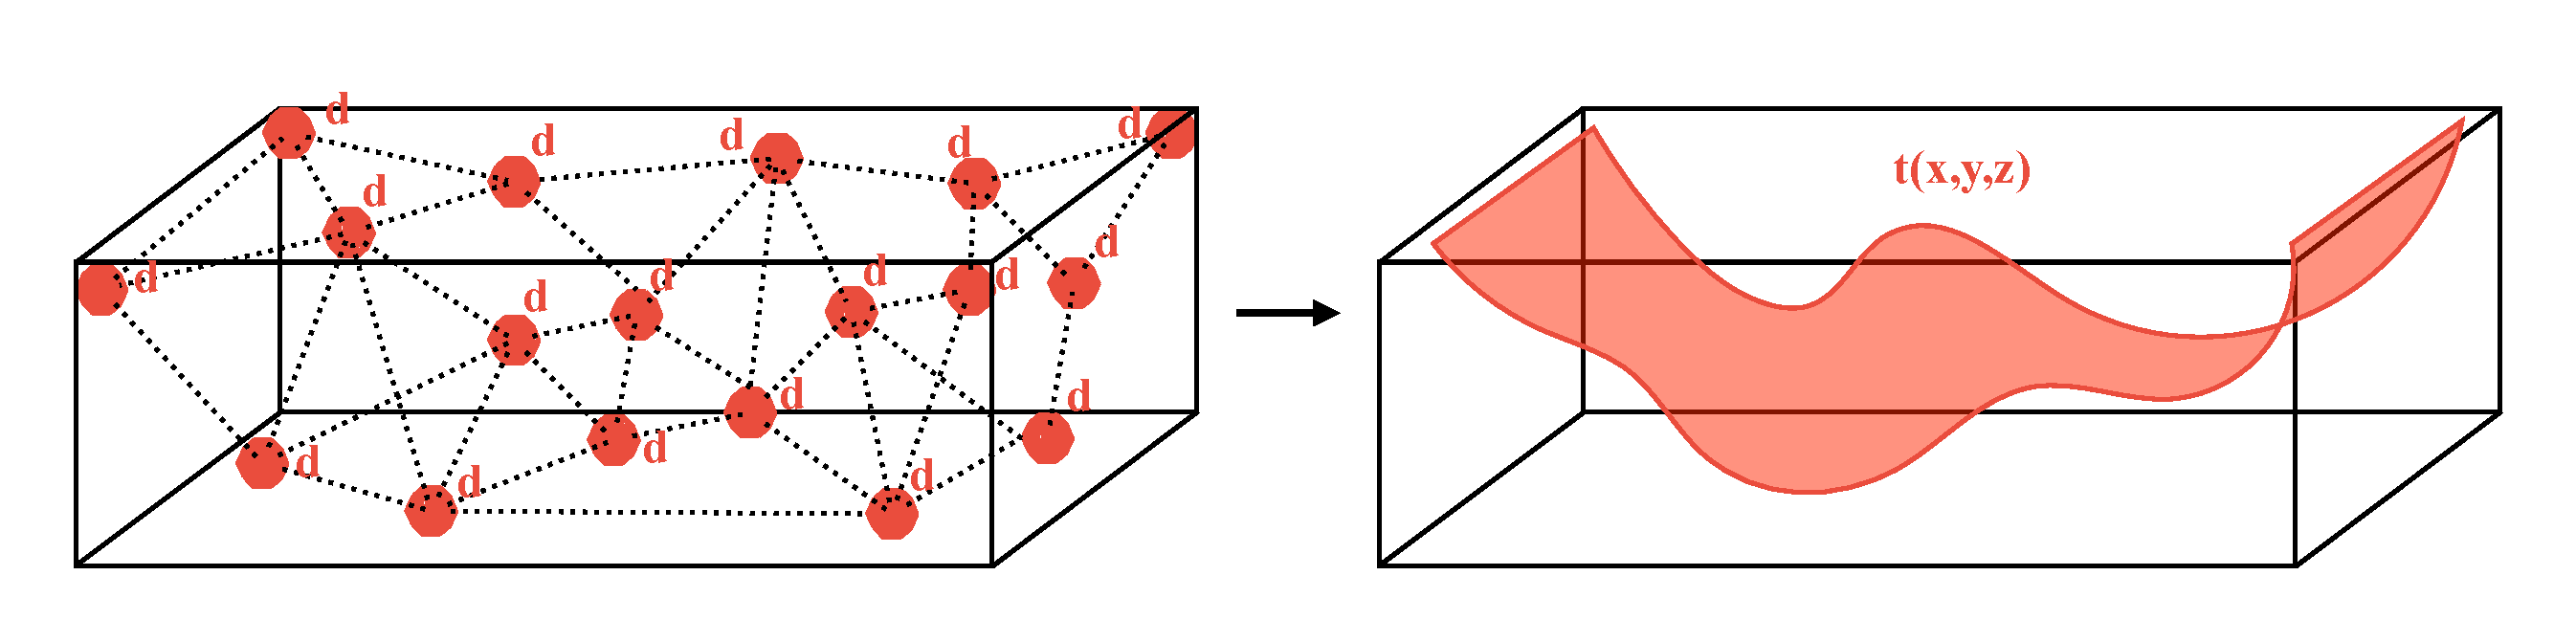
\includegraphics[width=.9\linewidth]{figures/points-to-gradient.pdf}
    \caption{Da sensori di temperatura $d_i \thinspace \forall i \in {\text{\{Insieme dei sensori.\}}}$ a spazio continuo di temperatura $t(x,y,z)$.}
    \label{fig:points-to-linear}
\end{figure}

\begin{figure}
    \centering
    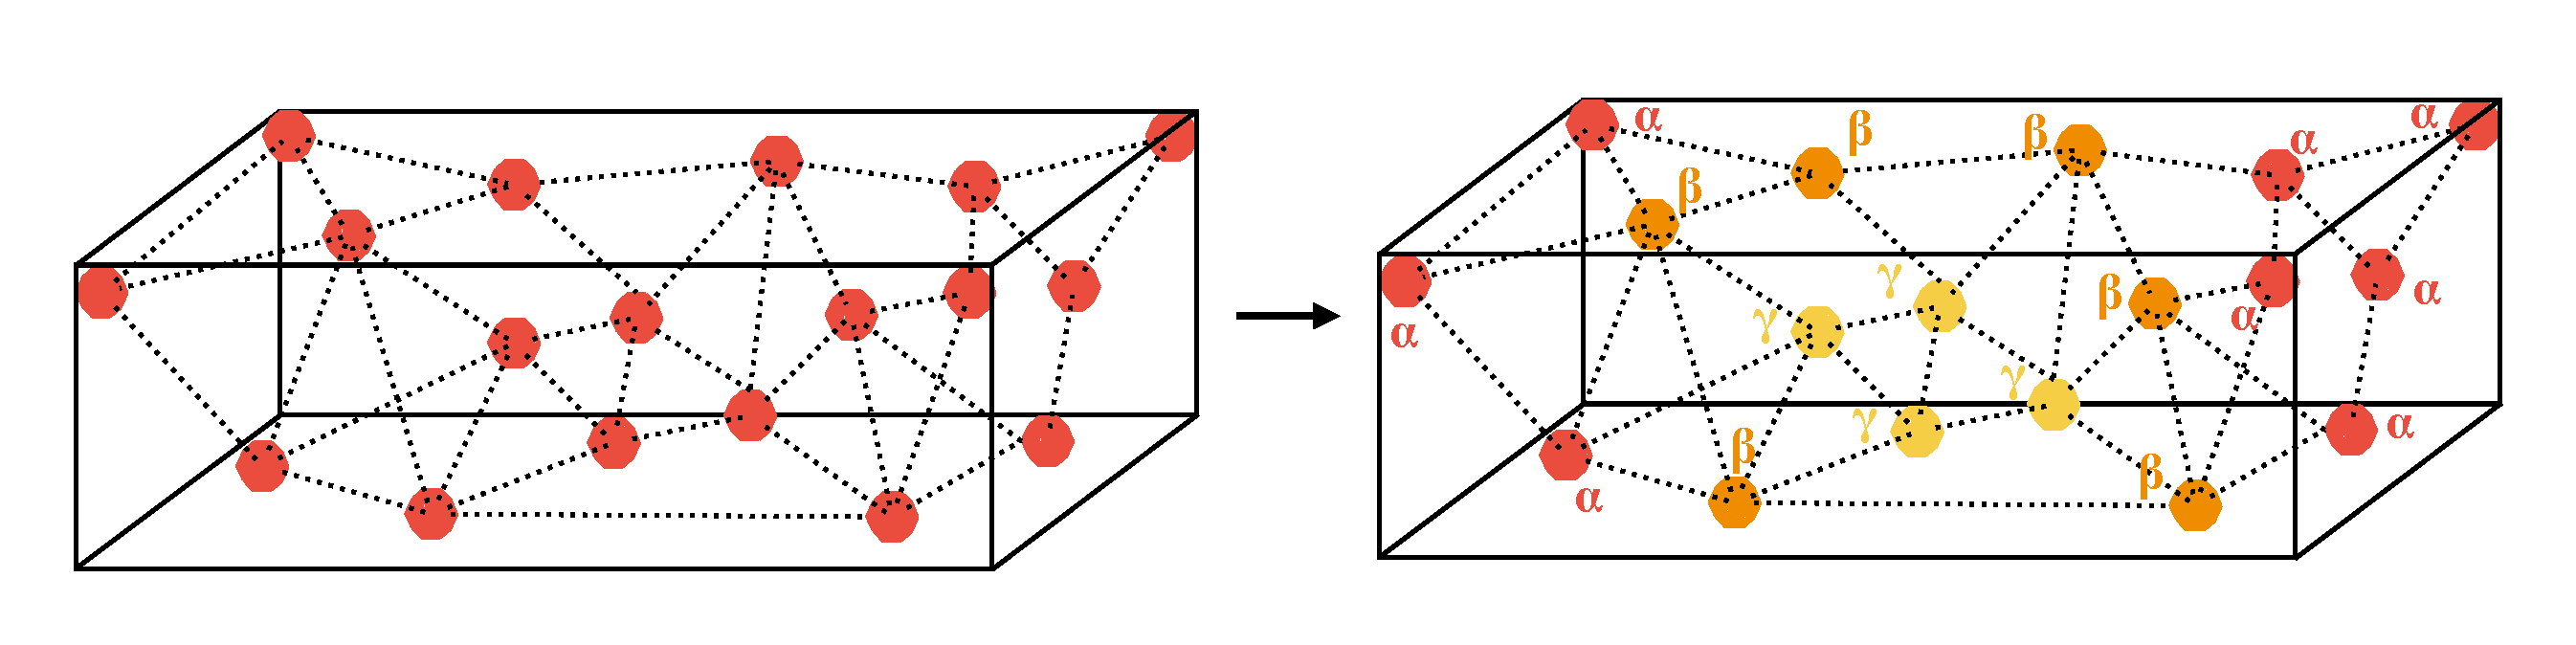
\includegraphics[width=.9\linewidth]{figures/different-function.pdf}
    \caption{Manipolazioni diverse in base al luogo. In questo caso sensori più vicini al centro della stanza hanno un comportamento diverso rispetto a quelli più vicini alle pareti.}
    \label{fig:different-function}
\end{figure}

\begin{figure}
    \centering
    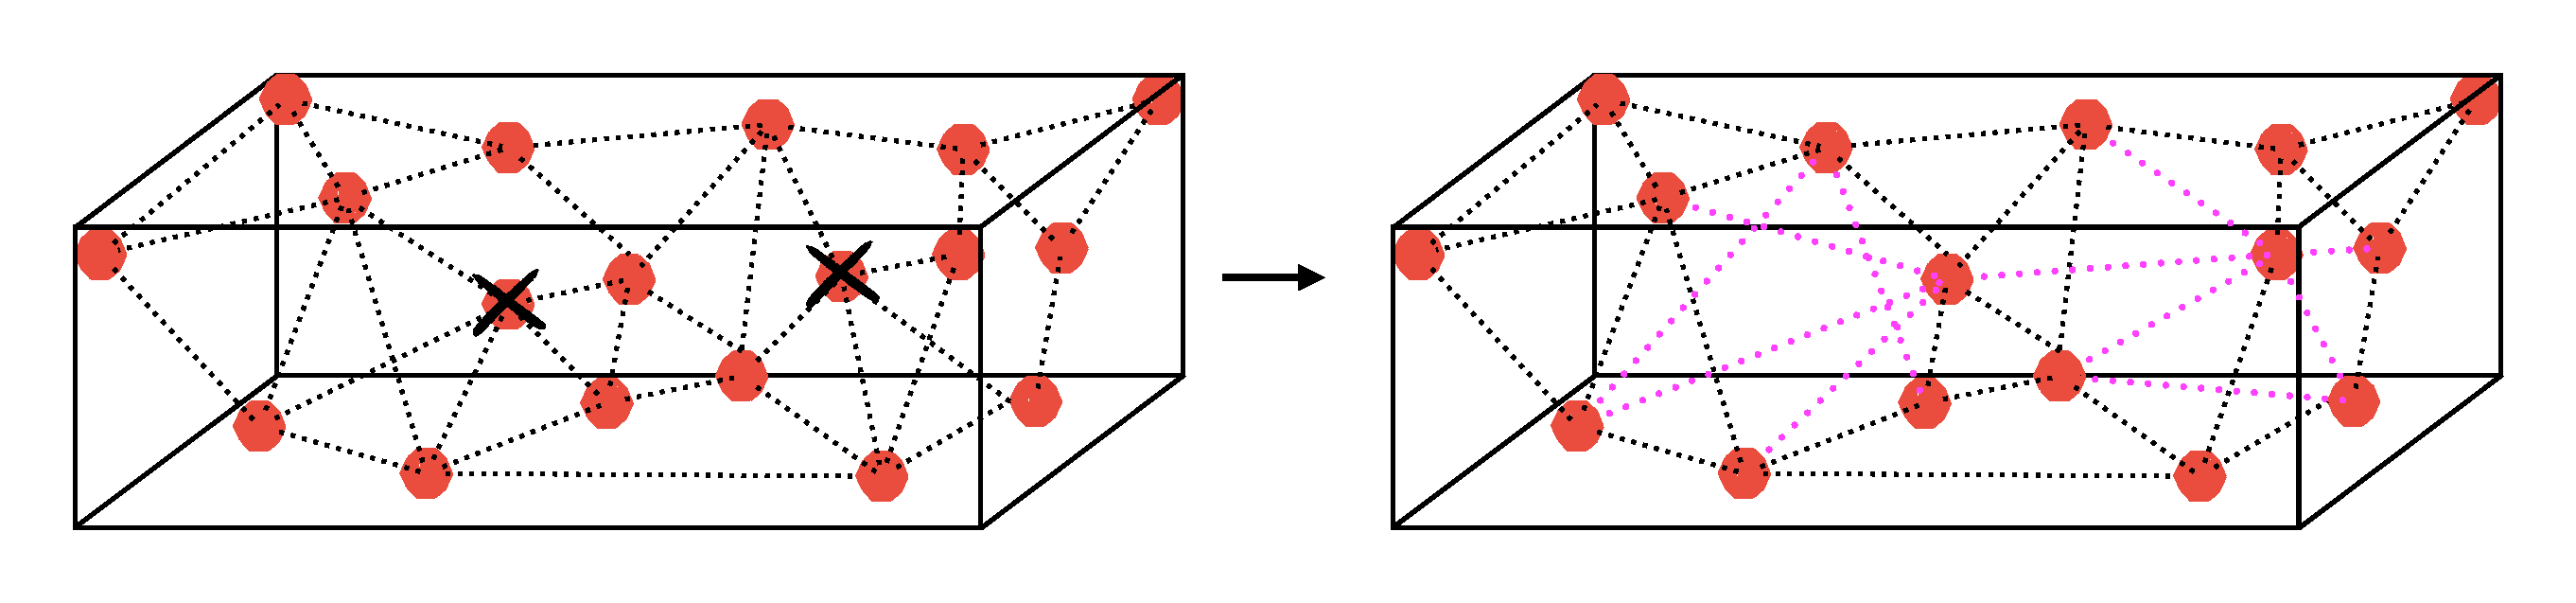
\includegraphics[width=.9\linewidth]{figures/lost-nodes.pdf}
    \caption{Sistema che si adatta alla perdita di nodi inserendo nuovi collegamenti.}
    \label{fig:lost-nodes}
\end{figure}

Dalla tecnologia dell'Aggregate Computing nasce anche la volontà di definire un metodo per la programmazione di sistemi aggregati: l'Aggregate Programming (AP). 
L'approccio \ac{AP} nella progettazione di sistemi è profondamente diverso classico approccio ``dispositivo centrico''.
Nel secondo caso, ogni dispositivo della rete ha il compito di compiere tutte le operazioni richieste per il raggiungimento della soluzione e simultaneamente comunicare con gli altri dispositivi della rete. Questo approccio, seppur semplice, è poco scalabile e difficile da mantenere al crescere della complessità del sistema \cite{Pianini2017}. 

% //TODO: capire cosa ho scritto e se ha senso quello scritto qui sotto
% Il nuovo paradigma, invece, prevede la scomposizione in componenti del programma assegnato ad ogni dispositivo, ogni componente esegue un compito specifico e comunica principalmente solo con i componenti dello stesso tipo presenti nel suo intorno per eseguire un servizio ed eventualmente con un altro componente presente nello stesso dispositivo al fine di realizzare una nuova soluzione inerente ad un'altro servizio. Le componenti sono una astrazioni dei \textit{campi di calcolo}.

Per \textit{campi computazionali} o \textit{computational fields} si intende la mappatura degli elementi del dominio in cui si opera in un insieme di valori come in figura \ref{fig:device-to-value}.
I campi vengono utilizzati per standardizzare le interazioni tra i dispositivi, permettendo di analizzare e progettare sistemi distribuiti in modo più semplice e intuitivo. L'idea di campo prende ispirazione dai campi fisici, come quello magnetico o quello gravitazionale. Ogni dispositivo della rete è considerato come un punto nello spazio ed il campo rappresenta un dato valore assegnato ad ognuno di questi punti. I campi, quindi, rappresentano un'astrazione ad alto livello dei dispositivi. L'insieme dei valori restituiti dalla mappatura rappresenta lo stato di un sistema in un dato istante \cite{Audrito2019}.

\begin{figure}
    \centering
    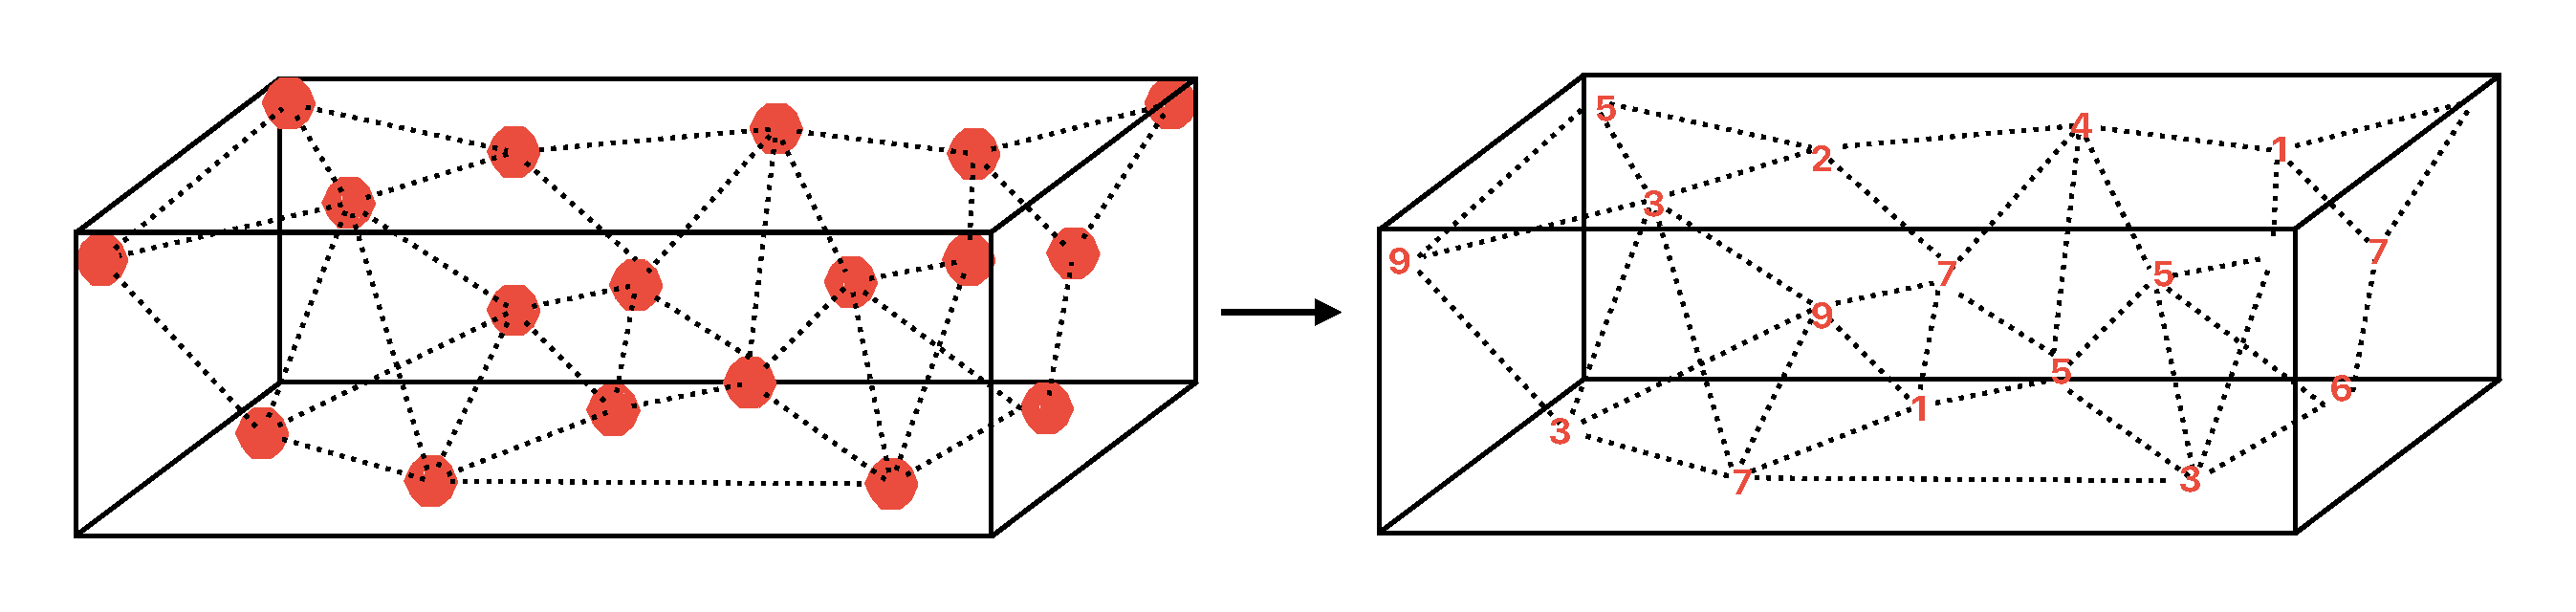
\includegraphics[width=.9\linewidth]{figures/device-to-value.pdf}
    \caption{Da dispositivi $d_i \thinspace \forall i \in {\text{\{Insieme dei dispositivi.\}}}$ a valori $f(d_i)$.}
    \label{fig:device-to-value}
\end{figure}

Questo approccio è generalmente utilizzato per un controllo prolungato dei dispositivi della rete. È ideale per reti di dispositivi sulle quali si vuole eseguire task che necessitano un gran numero di rilevazioni (utilizzando sensori), computazioni ed attuazioni nello spazio e nel tempo.

Ogni dispositivo del proprio sistema aggregato esegue una computazione in modo asincrono attraverso i \textbf{sense-compute-(inter)act rounds}\label{sec:sense-compute-interact} \cite{Macroswarm}, ogni round è composto da tre fasi concettuali (figura \ref{fig:sca-round}) \cite{Casadei2021-2}:

\begin{enumerate}
    \item \textbf{Aggiornamento del contesto (sense)}: ogni nodo memorizza il suo stato precedente, i dati ambientali restituiti da eventuali sensori e le più recenti informazioni ricevute dai nodi vicini.
    \item \textbf{Esecuzione del Programma Aggregato (compute)}: il campo di ogni nodo viene computato in base al contesto locale e produce un valore di output detto \textit{export} da condividere con il proprio vicinato ed un output utile per l'attuazione.
    \item \textbf{Azione (inter-act)}: in questa fase il nodo effettua le seguenti azioni:
    \begin{enumerate}
        \item \textbf{Condivisione}: il nodo condivide il proprio \textit{export} verso i nodi del suo vicinato in formato broadcast
        \item \textbf{Controllo attuatori}: l'output del nodo \\ viene 
        utilizzato per l'esecuzione di uno o più attuazioni nel proprio ambiente
    \end{enumerate}
\end{enumerate}

\begin{figure}
    \centering
    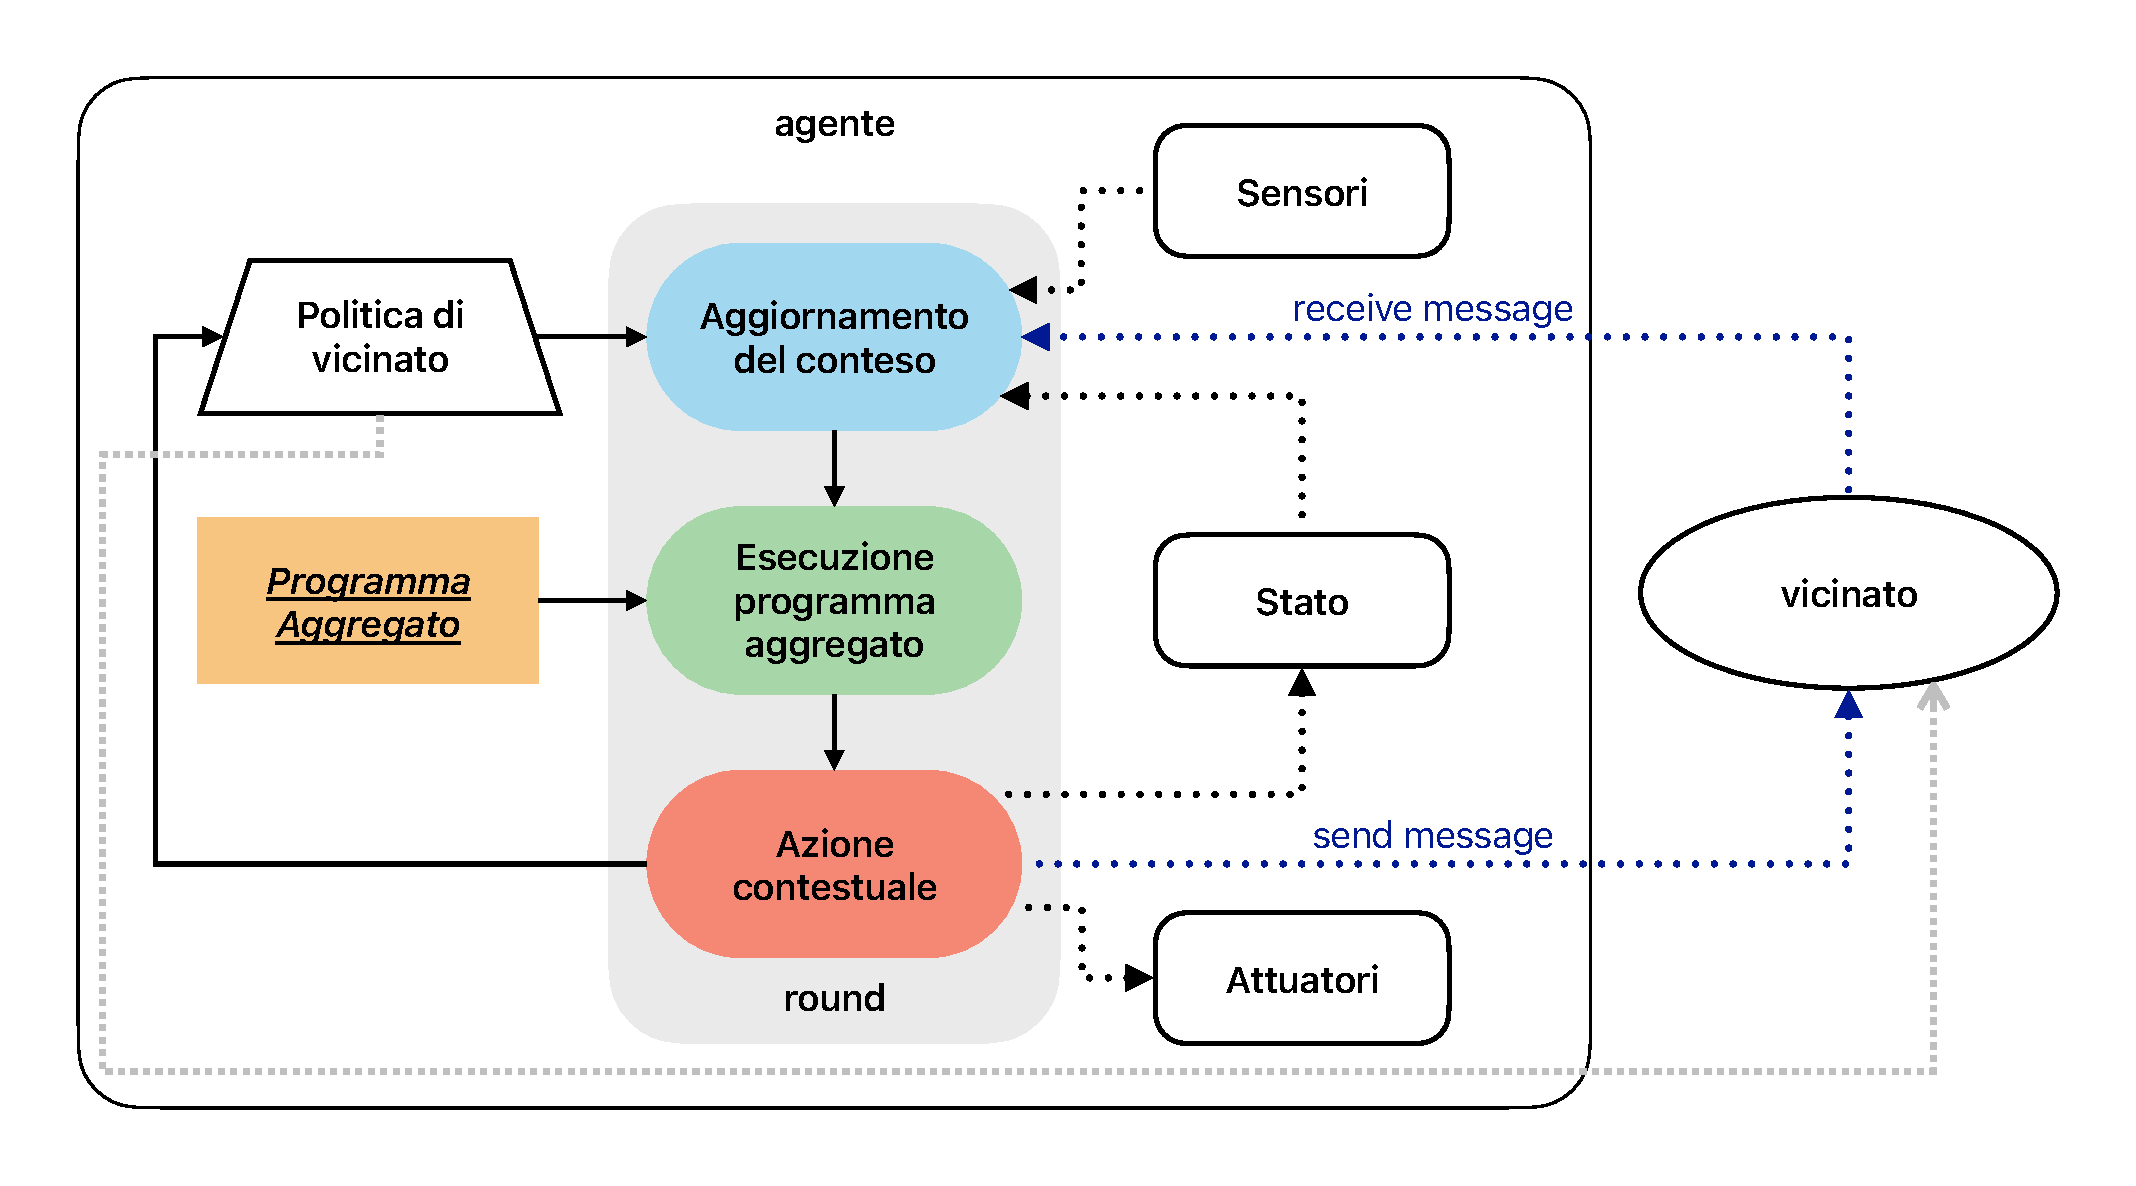
\includegraphics[width=.9\linewidth]{figures/sca-round.pdf}
    \caption{Fasi di un round di computazione in un sistema aggregato.}
    \label{fig:sca-round}
\end{figure}

Posizionandoci in un livello più implementativo troviamo i seguenti costrutti per la manipolazione dei campi \cite{Pianini2017}: 

\begin{itemize}
    \item \textbf{Functions}: funzioni $$ b(e_1,\dots,e_n) $$ applicate agli argomenti $e_1,\dots,e_n$. Possono essere sia funzioni matematiche, logiche o algoritmiche ma possono anche rappresentare sensori o attuatori.
    \item \textbf{Dynamics}: $$ rep(x \leftarrow v){s_1;\dots;s_n} $$ rappresenta un una variabile di stato locale $x$, inizialmente inizializzata con il valore $v$ e che può essere modificata dalle istruzioni $s_1,\dots,s_n$. In questo modo si definisce un campo dinamico.
    \item \textbf{Interaction}: $$ nbr(s) $$ permette di fare una query di un certo valore rispetto al vicinato 
% //TODO: ristudiare e sistemare Interaction
    \item \textbf{Restrictions}: $$
        \begin{array}{l}
        \text{if } e \\
        \qquad s_1; \quad \dots \quad s_n; \\
        \text{else} \\
        \qquad s_1'; \quad \dots \quad s_m';
        \end{array}
    $$
    permette di andare a definire sotto spazio del campo principiale in base ad una condizione $e$ sul quale poi andare ad eseguire certe istruzioni invece di altre. È importante che le istruzioni riferite ad un certo sotto spazio non abbiano effetti su altri sotto spazi.
\end{itemize}

Le tecnologie sviluppate con approccio \ac{AP} non sono prive di difetti. 
Implementazioni di questo tipo sono difficili da integrare in sistemi già programmati in modo più tradizionale, inoltre, dal punto di vista della programmazione sono mancanti i meccanismi per la gestione della concorrenza e della computazione dinamica dei campi. Il framework ScaFi, che vedremo nel prossimo capitolo, cerca di risolvere questi problemi.

% //TODO: capitolo incompleto ?

\section{ScaFi}

ScaFi è un toolkit open-source scritto in linguaggio Scala ideato per lo sviluppo ad alto livello di sistemi aggregati. Questo toolkit è costruito sulle basi dell'Aggregate Programming ed il termine ScaFi deriva dalla unione di \textbf{Scala} e \textbf{Fields}. Il termine Field deriva dai \textit{field calculus} di cui abbiamo parlato nei capitoli precedenti.

L'Architettura di ScaFi \cite{Casadei2022} è riassumibile nella immagine \ref{fig:scafi-arc}.

\begin{figure}
    \centering
    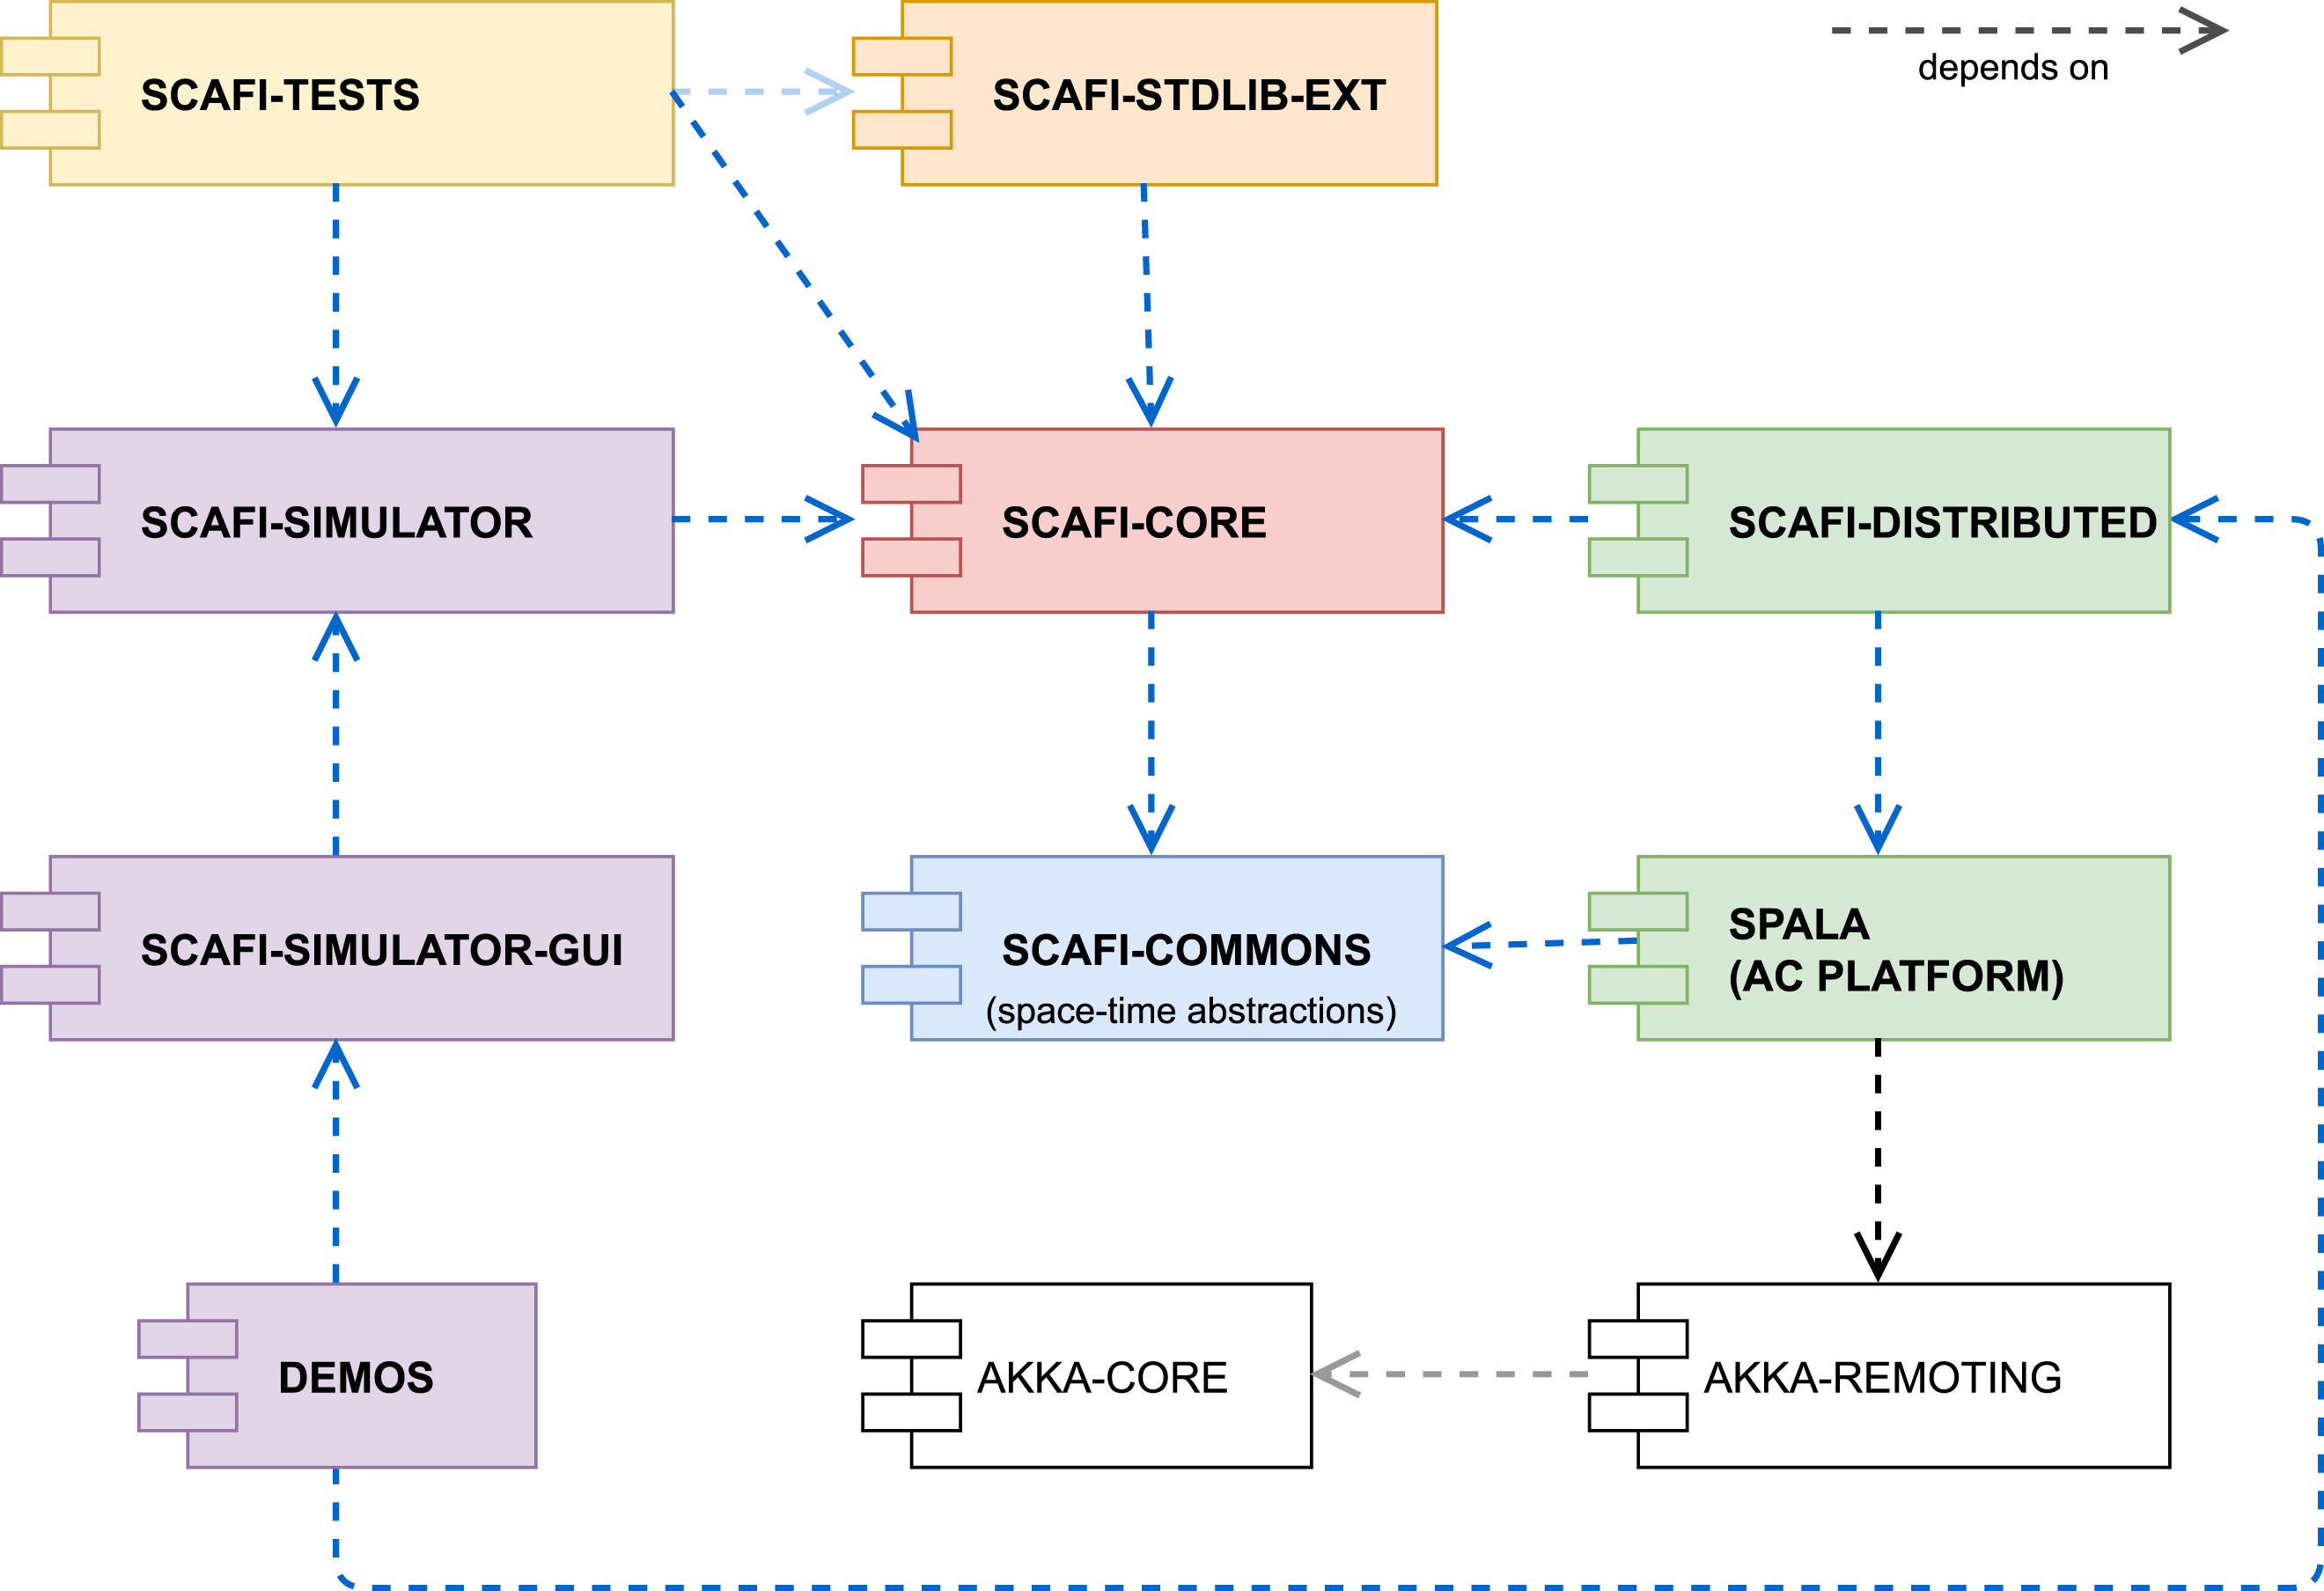
\includegraphics[width=.8\linewidth]{figures/scafi-arc.jpg}
    \caption{Architettura ad alto livello del framework ScaFi}
    \label{fig:scafi-arc}
\end{figure}

Ispezionando la figura, troviamo:

\begin{itemize}
    \item \textbf{scafi-commons}: fornisce le entità di base, ad esempio astrazioni temporali e spaziali
    \item \textbf{scafi-core}: rappresenta il core del framework fornendo il DSL\footnote{Domain Specific Language: linguaggio di programmazione progettato specificamente per risolvere problemi o esprimere concetti di un dominio ristretto. Il DSL di ScaFi (libreria di programmazione) è quindi un linguaggio specifico per creare e valutare programmi di tipo aggregato, utilizzando una sintassi e una semantica pensate appositamente per questo tipo di calcoli e simulazioni.} per la progettazione di sistemi aggregati; con il supporto di librerie standard.
    \item \textbf{scafi-simulator}: fornisce un supporto per la simulazione dei sistemi di \ac{AP} sviluppati
    \item \textbf{scafi-simulator-GUI}: fornisce un'interfaccia grafica per la simulazione
    \item \textbf{spala}: (``spatial scala'') si tratta di un \textit{middleware} che permette di eseguire programmi \ac{AC} basati sugli attori ed è indipendente dal DSL di ScaFi
    \item \textbf{scafi-distributed}: layer integrativo per l'utilizzo di \textbf{spala} in ScaFi
\end{itemize}

\paragraph{scafi-core} Questo modulo (figura \ref{fig:core-arc}) espone l'incarnazione dell'interfaccia di un \textbf{AggregateProgram}, questo singolo programma si occupa di definire l'intera operatività del insieme dei dispositivi della rete. Andare ad assemblare una sottoclasse di \verb|AggregateProgram| con l'interfaccia \verb|Gradients| permette di creare una funzione di gradiente che si sviluppa (nello spazio e nel tempo) partendo dai nodi sorgente ed espandendosi verso i nodi destinazione.

\begin{figure}
    \centering
    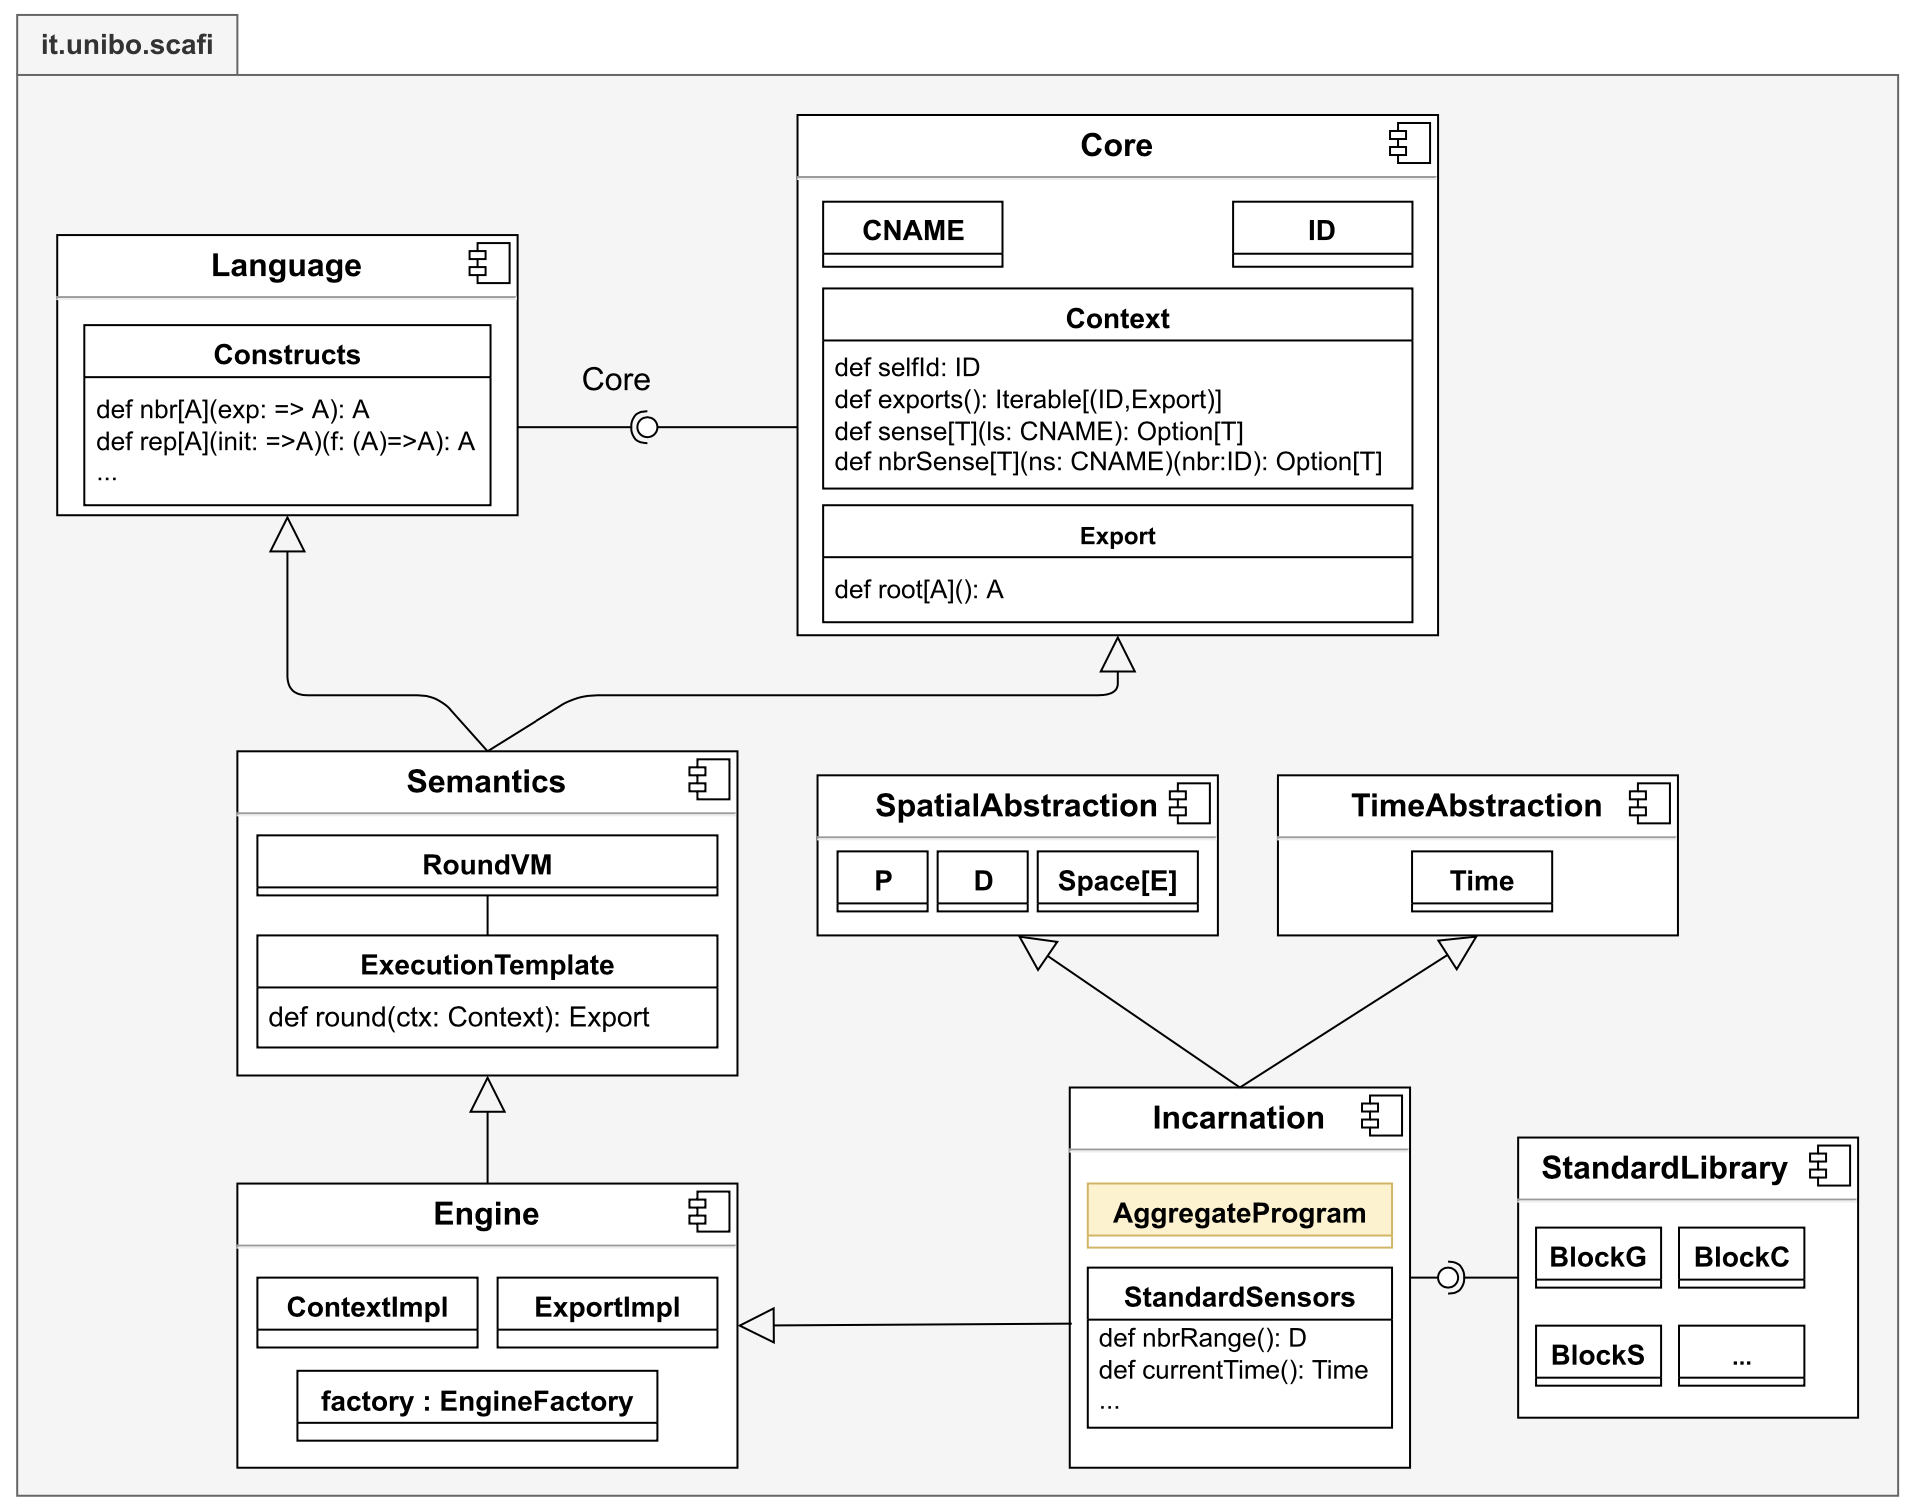
\includegraphics[width=.9\linewidth]{figures/core-arc.png}
    \caption{Architettura del modulo scafi-core}
    \label{fig:core-arc}
\end{figure}

Di seguito l'interfaccia fondamentale per la definizione di un campo di calcolo in Scala (\cref{lst:constructs-scala}):

\lstinputlisting[float=tb,language=Scala,label={lst:constructs-scala},caption={Interfaccia per la definizione di un campo di calcolo in Scala}]{listings/Constructs.scala}

Gli elementi principali di questa interfaccia sono \cite{Casadei2022}:
\begin{itemize}
    \item \verb|rep(init)(f)| cattura l'evoluzione di stato di un valore inizializzato ad \verb|init| e aggiornato ad ogni round con la funzione \verb|f|
    \item \verb|nbr(expr)|: rileva le comunicazioni relative al valore computato dalla espressione \verb|expr| dei nodi vicini
    \item \verb|foldhood(init)(acc)(expr)|: si occupa, partendo da un valore iniziale \verb|init|, di accumulare i valori computati dai nodi vicini attraverso la funzione di accumulazione \verb|acc| e settare i valori computati dalla espressione \verb|expr| verso i propri vicini
    \item \verb|branch(cond)(th)(el)|: cattura una partizione (spazio-temporale) del dominio in base alla condizione \verb|cond|, se questa è rispettata esegue l'espressione \verb|th| altrimenti \verb|el|
    \item \verb|mid|: provvede ad identificare un certo nodo
    \item \verb|sense(sensorName)|: permette di accedere (ad alto livello) al sensore locale \verb|sensorName|
    \item \verb|nbrvar(sensorName)|: permette di accedere (ad alto livello) ai sensori dei nodi vicini, simile ad \verb|nbr| ma valido per sensori forniti dalla piattaforma, questi sensori forniscono un valore per ciascun vicino
\end{itemize}

In ScaFi, i campi non sono reificati esplicitamente ma esistono solo a livello semantico, questo significa che un'espressione Scala non viene gestita come un'espressione di campo finché non viene passata all'interprete ScaFi \cite{CasadeiPhDThesis}.

ScaFi fornisce alcuni operatori di alto livello per la sviluppo di comportamenti collettivi \cite{Casadei2022} (le immagini sono tratte da \cite{CasadeiPhDThesis}):

\begin{itemize}
    \item \textbf{Leader election (definizione di un leader)}: Blocco 
    \begin{center}
        \verb|S(grain: Double):Boolean|
    \end{center}
    produce un campo booleano auto organizzato che definisce a \verb|true| un insieme sparso di dispositivi distanziati tra di loro di almeno \verb|grain| (figura \ref{fig:leader-election}).
    \item \textbf{Gradient-cast (propagazione distribuita)}: Blocco 
    \begin{center}
        \verb|G[T](source: Boolean, value: T, acc: T=>T): T|
    \end{center}
    utilizzato per propagare un valore \verb|value| da una sorgente \verb|source| a tutti i nodi della rete, in ordine di distanza crescente, seguendo un gradiente, che modifica i valori di ogni nodo secondo una funzione di accumulo \verb|acc|. Un gradiente è una variazione continua di una quantità rispetto a una direzione. In ambito matematico e fisico, indica la direzione e la rapidità con cui una grandezza scalare come temperatura, pressione o colore in una mappa variano nello spazio (figura \ref{fig:gradient-cast}).
    \item \textbf{Collect-cast (collezione distribuita)}: Blocco 
    \begin{center}
        \verb|C[T](sink: Boolean, value: T, acc(T,T)=>T): T| 
    \end{center}
    utilizzata per riassumere le informazioni distribuite in un unico dispositivo \verb|sink|, i valori \verb|values| prodotti dai dispositivi vengono ``raccolti'' dal gradiente che si muove in direzione di \verb|sink| e vengono accumulati secondo la funzione di accumulo \verb|acc| (figura \ref{fig:collect-cast}).
\end{itemize}

\begin{figure}[H]
    \centering
    \begin{minipage}[b]{0.3\textwidth}
        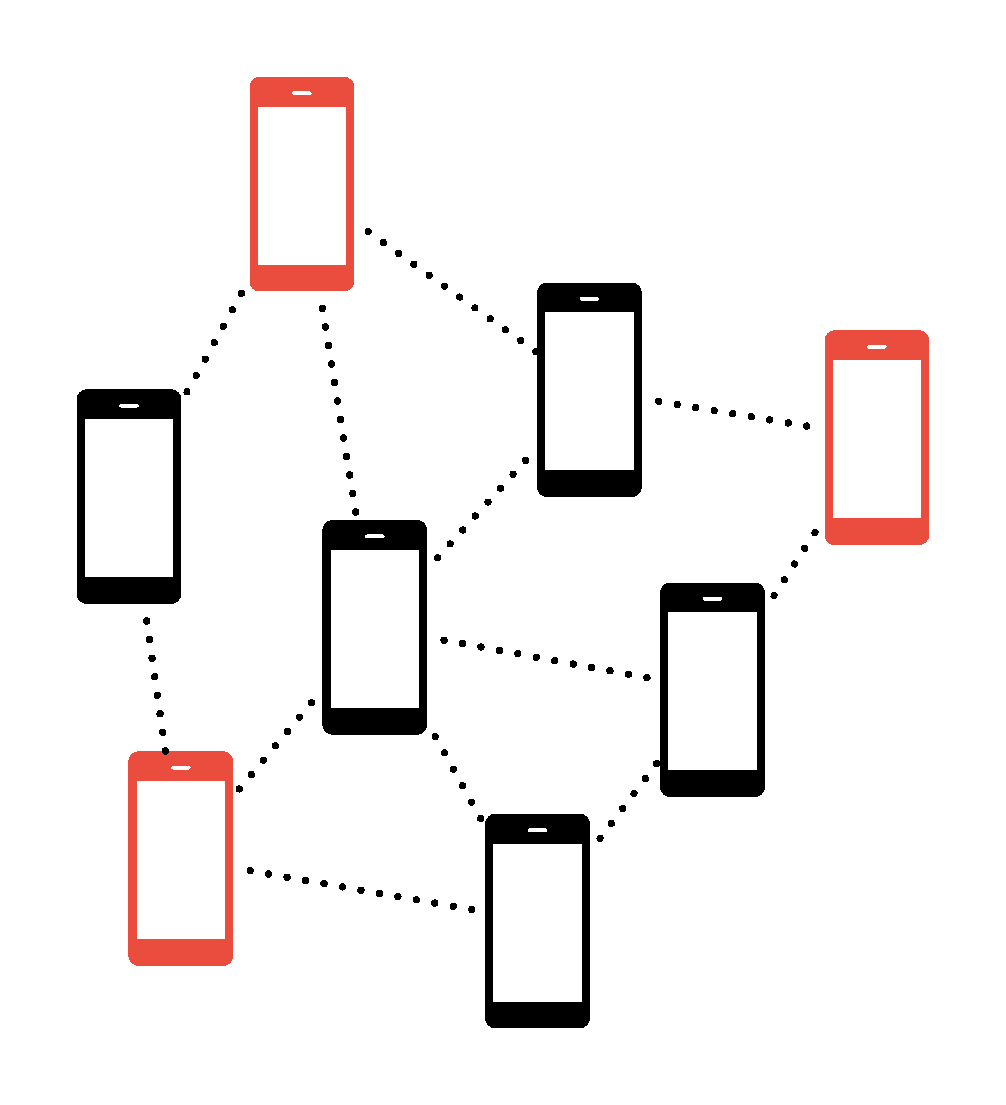
\includegraphics[width=\textwidth]{figures/leader-election.pdf}
        \caption{Leader election}
        \label{fig:leader-election}
    \end{minipage}
    \hfill
    \begin{minipage}[b]{0.3\textwidth}
        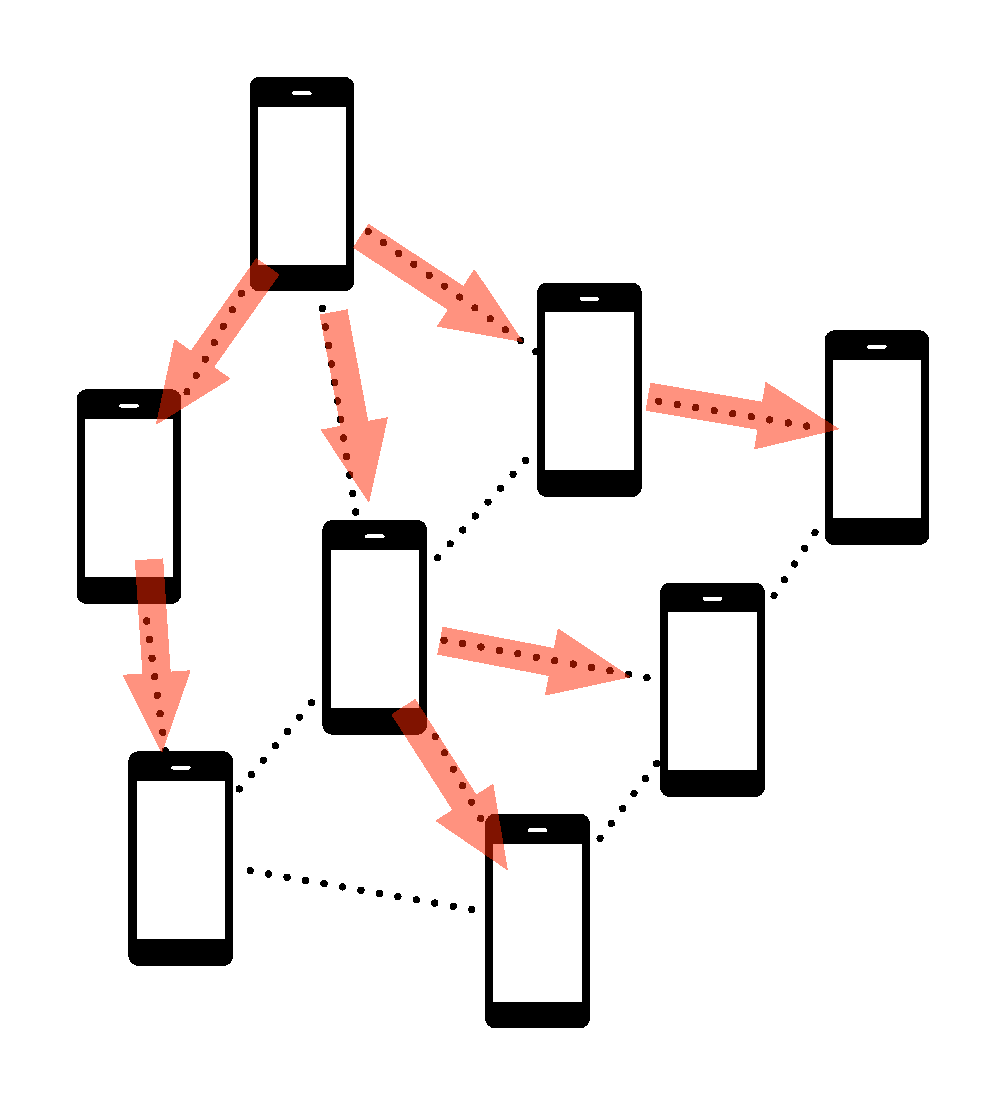
\includegraphics[width=\textwidth]{figures/gradient-cast.pdf}
        \caption{Gradient cast}
        \label{fig:gradient-cast}
    \end{minipage}
    \hfill
    \begin{minipage}[b]{0.3\textwidth}
        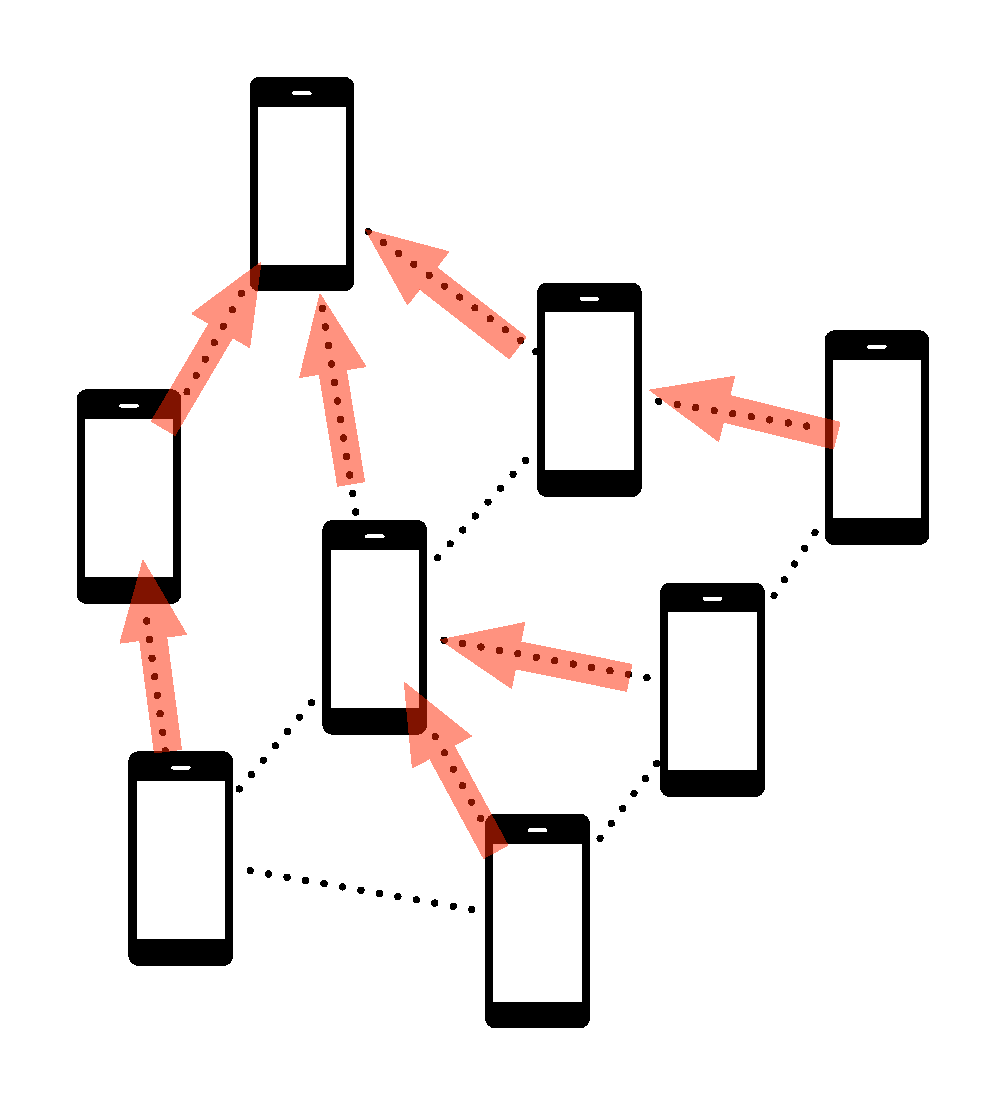
\includegraphics[width=\textwidth]{figures/collect-cast.pdf}
        \caption{Collect cast}
        \label{fig:collect-cast}
    \end{minipage}
\end{figure}

\section{Macroswarm}

Macroswarm è un framework che estende il toolkit ScaFi  per la programmazione di sistemi di robotica distribuita. Macroswarm nasce con l'avanzare delle tecnologie ed il crescente interesse verso il controllo di flotte di dispositivi come droni, robot, veicoli o folle di persone definite da dispositivi portatili/indossabili in modo.
Si è voluto, quindi, creare un framework che permettesse di programmare sistemi distribuiti di robot in modo semplice ed intuitivo secondo degli \textit{swarm behavior}\footnote{Comportamenti di sciame/flotta}, permettendo di concentrarsi solo sulla logica di alto livello del sistema. Questo framework è stato scelto per il progetto in esamina.

\begin{figure}
    \centering
    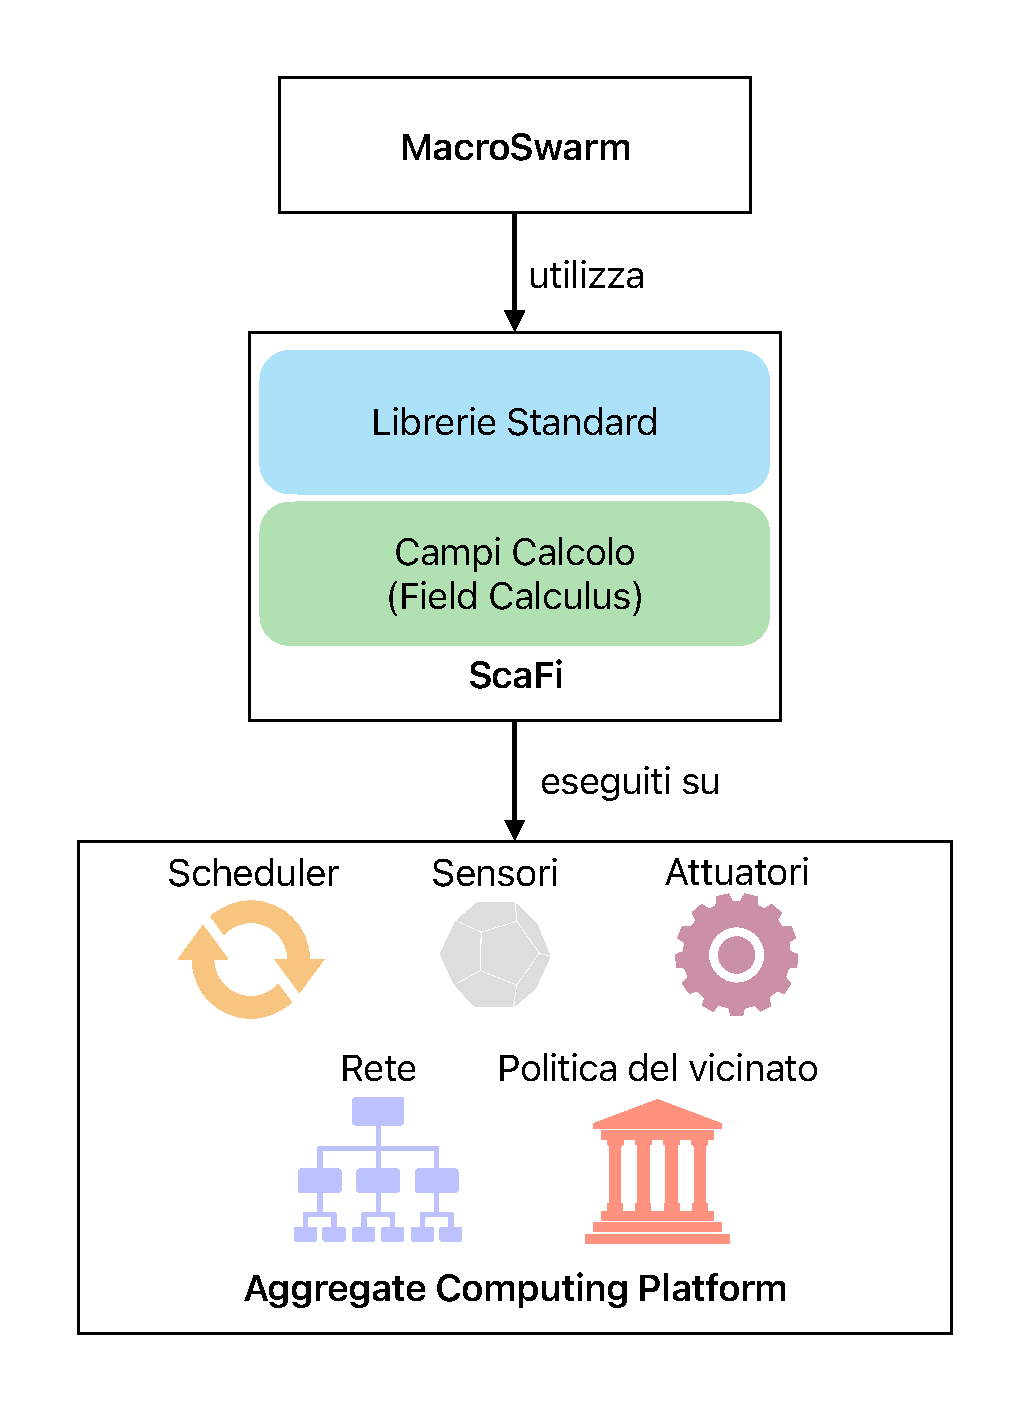
\includegraphics[width=.8\linewidth]{figures/macroSwarm-arc.pdf}
    \caption{Architettura di Macroswarm}
    \label{fig:macro-swarm-arc}
\end{figure}

Macroswarm semplifica lo sviluppo di sistemi aggregati fornendo un insieme di blocchi di alto livello che permettono di definire comportamenti di ``\textit{stormo}'' (come quello degli uccelli), comportamenti ``\textit{leader-follower}'' (come nei branchi di elefanti), comportamenti di auto-organizzazione, cambiamento strutturale e formazione di \textit{team} \cite{Macroswarm}.
I blocchi rappresentano le API per progettazione dei sistemi aggregati su sistemi fisici (i rettangoli bianchi in figura \ref{fig:macro-swarm-int} rappresentano i moduli principali). Questi blocchi rappresentano alcuni dei comportamenti essenziali, come vedremo nei prossimi paragrafi, per la ideazione di comportamenti più complessi la difficoltà rimane relativamente bassa poiché basterà comporre blocchi più semplici (come quelli già implementati) per ottenere il comportamento desiderato.

\begin{figure}
    \centering
    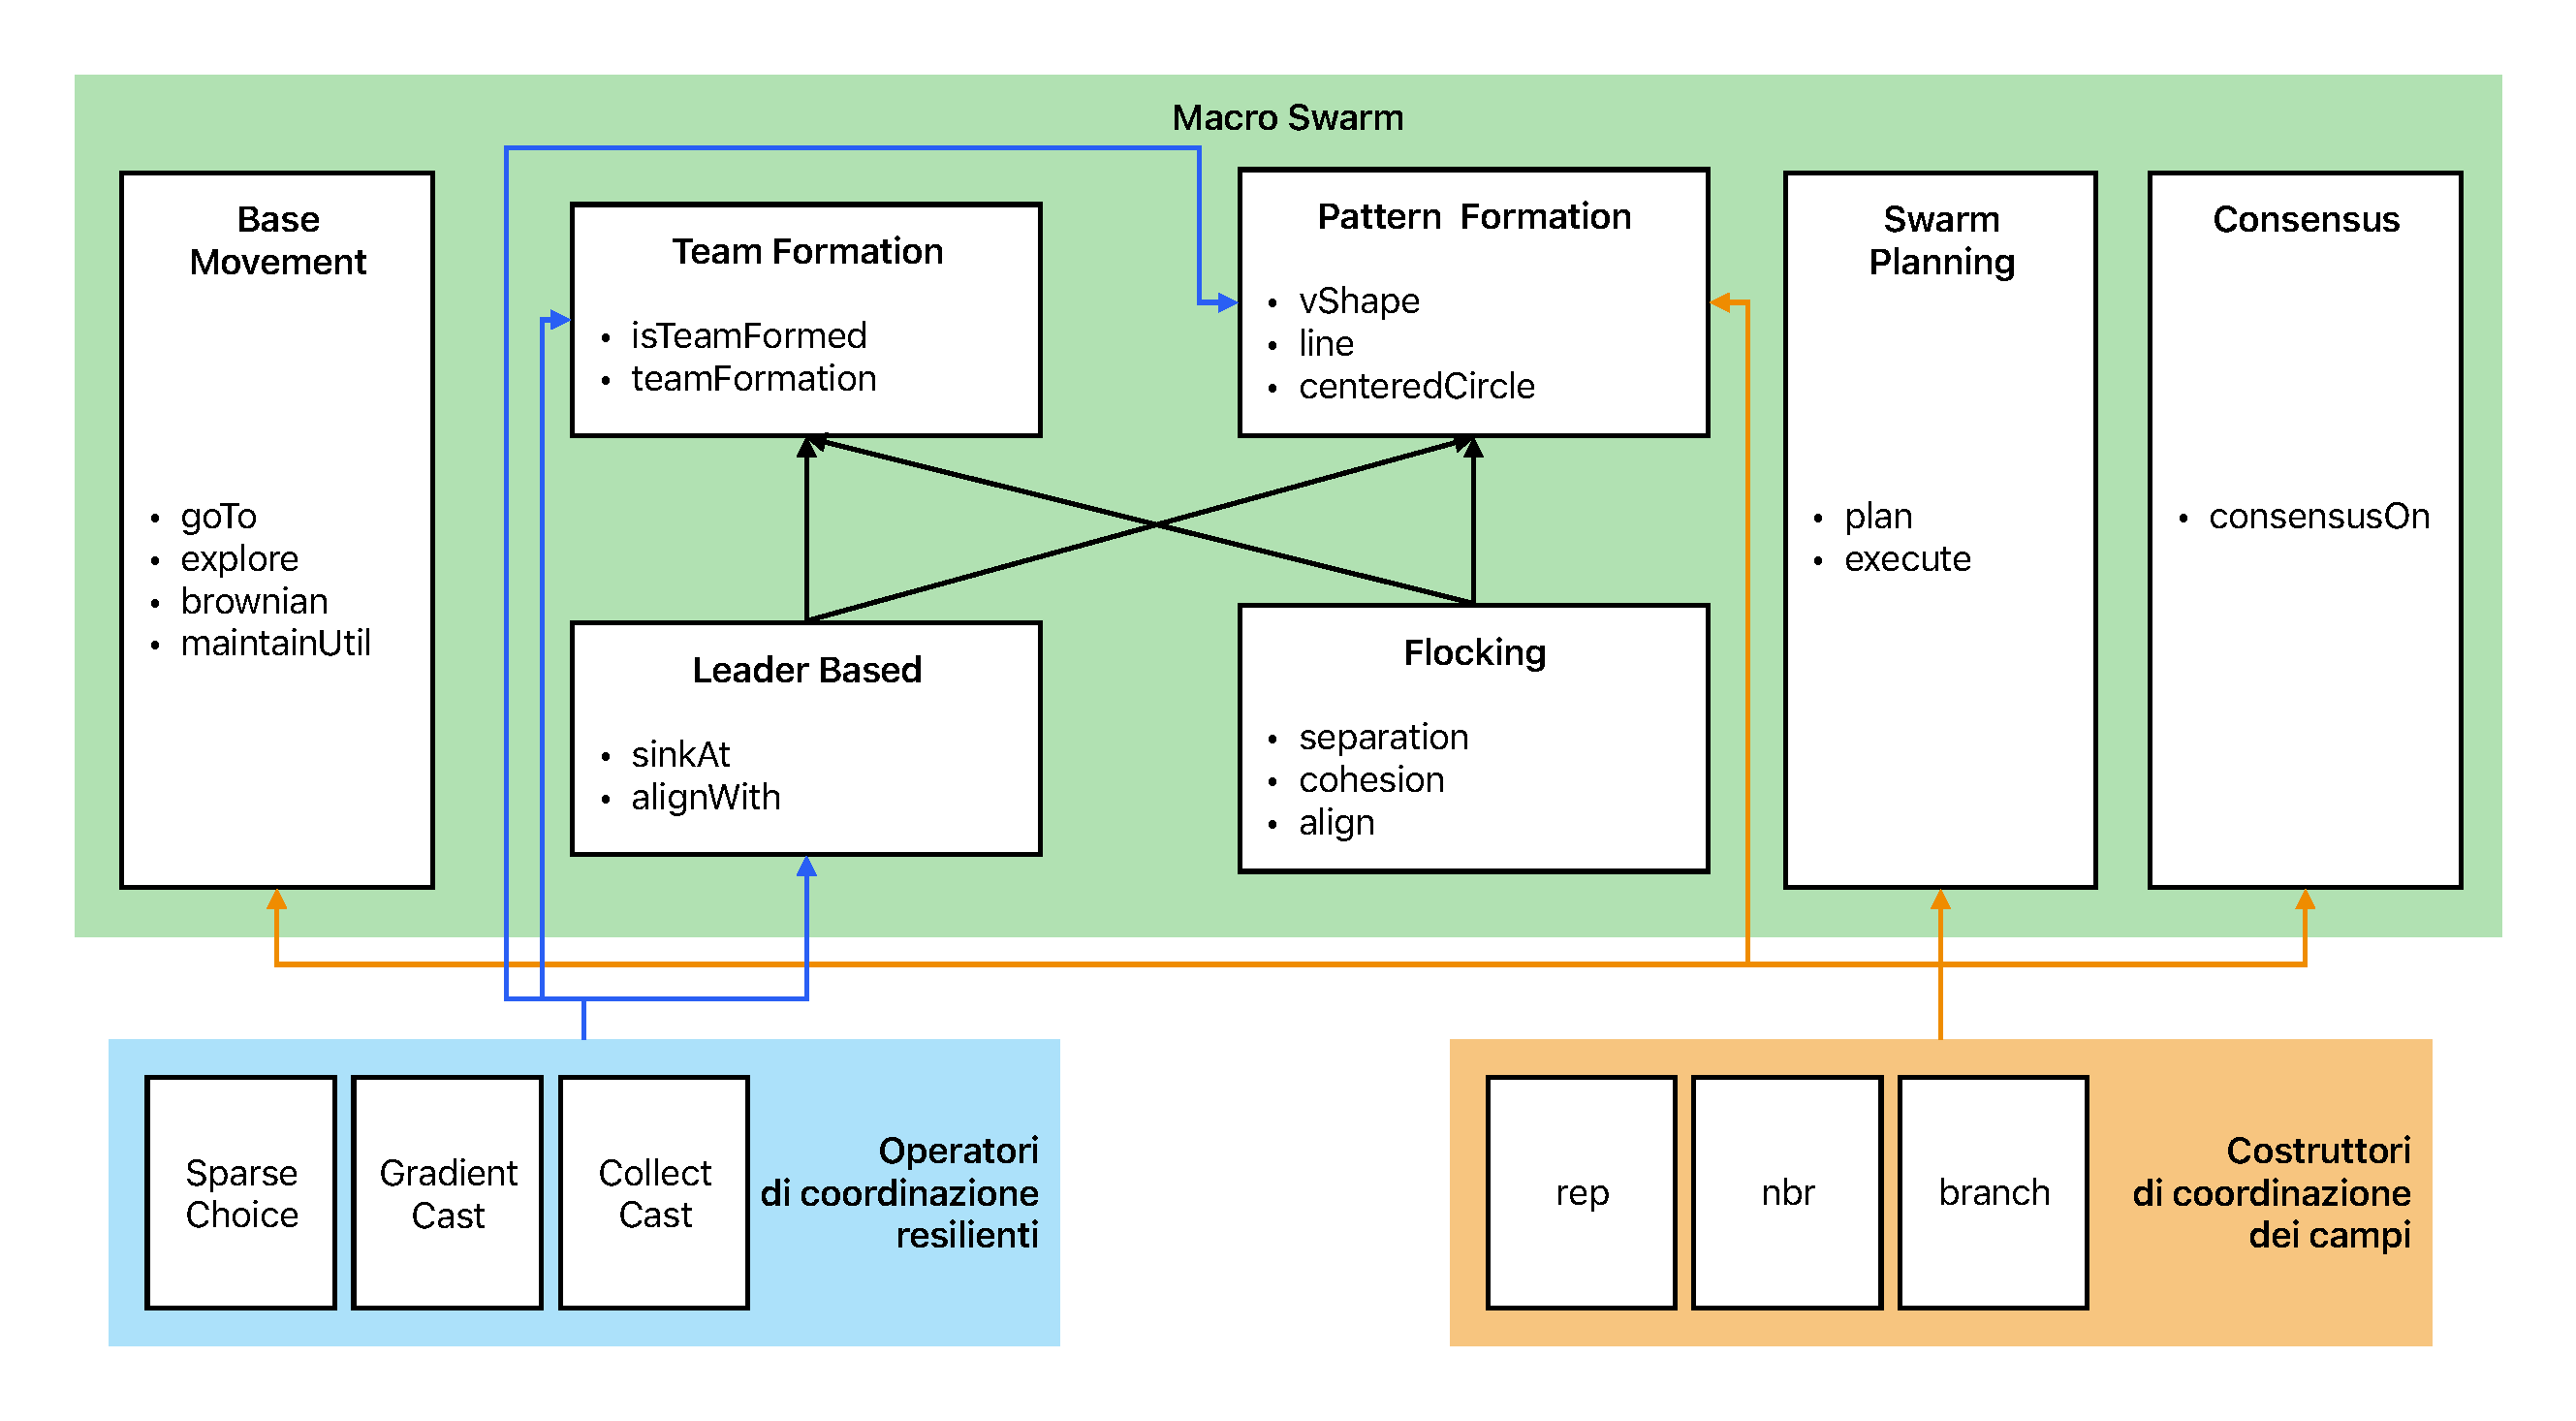
\includegraphics[width=.99\linewidth]{figures/macroSwarm-modeles.pdf}
    \caption{Struttura di Macroswarm e moduli interni}
    \label{fig:macro-swarm-int}
\end{figure}

È rilevante notare che in Macroswarm la computazione della attuazione da eseguire su un certo dispositivo e la reale attuazione nel mondo reale sono disaccoppiate. Il motivo di questa scelta è dovuto al fatto che ad ogni round\cref{sec:sense-compute-interact} il programma aggregato può variare un qualche parametro per completare il task. È, comunque, possibile scegliere quale modalità di computazione-attuazione scegliere poiché, in base al contesto, una può essere più adatta dell'altra \cite{Macroswarm}. Le modalità sono:

\begin{itemize}
    \item \textbf{round-based}(figura \ref{fig:round-based}): è possibile eseguire l'attuazione definita al termine del prossimo round 
    \item \textbf{long-standing}(figura \ref{fig:long-standong}): l'attuazione che si vuole eseguire è valida finché non viene revisionata o ritirata
\end{itemize}

\begin{figure}
    \centering
    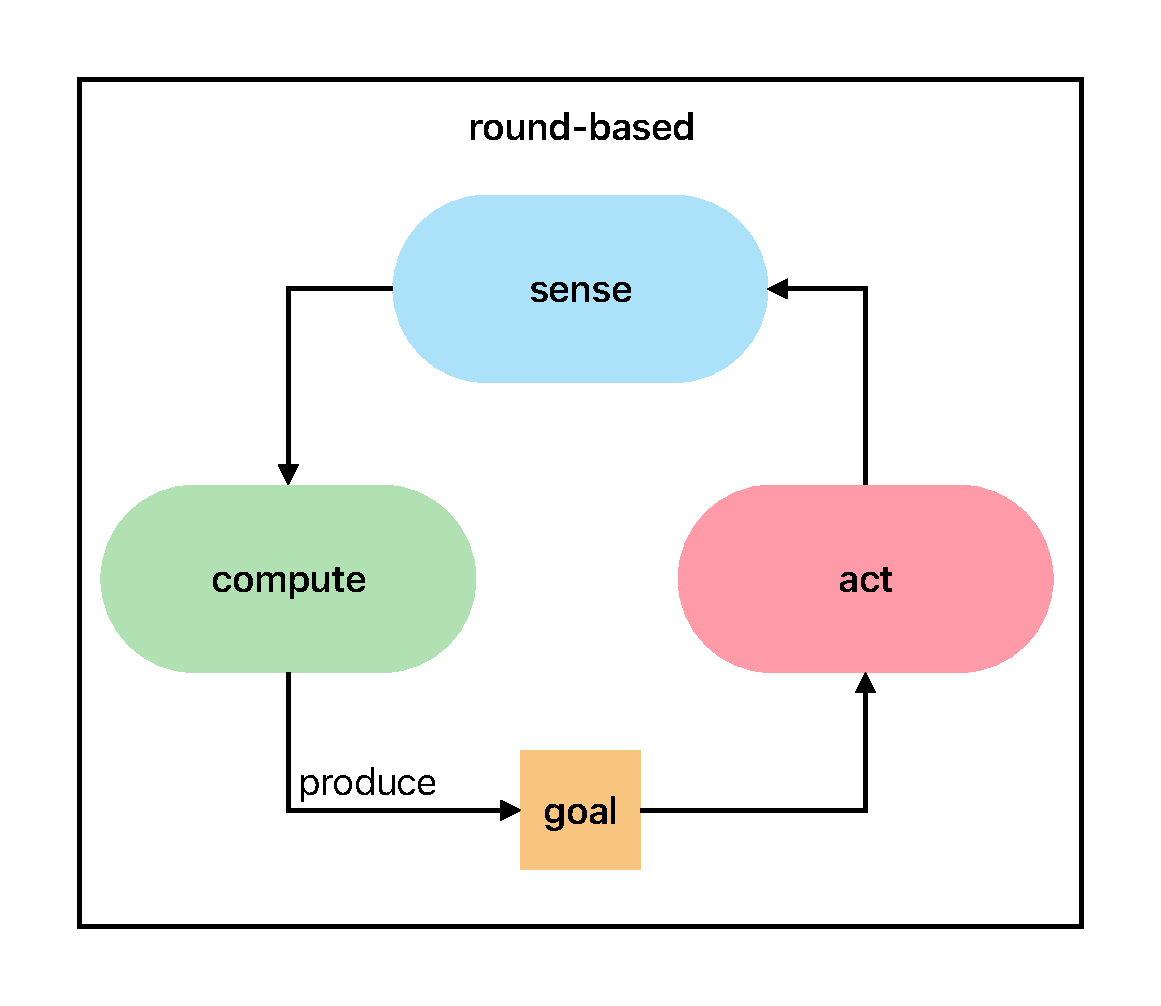
\includegraphics[width=.6\linewidth]{figures/round-based.pdf}
    \caption{Modalità Round Based}
    \label{fig:round-based}
\end{figure}

\begin{figure}
    \centering
    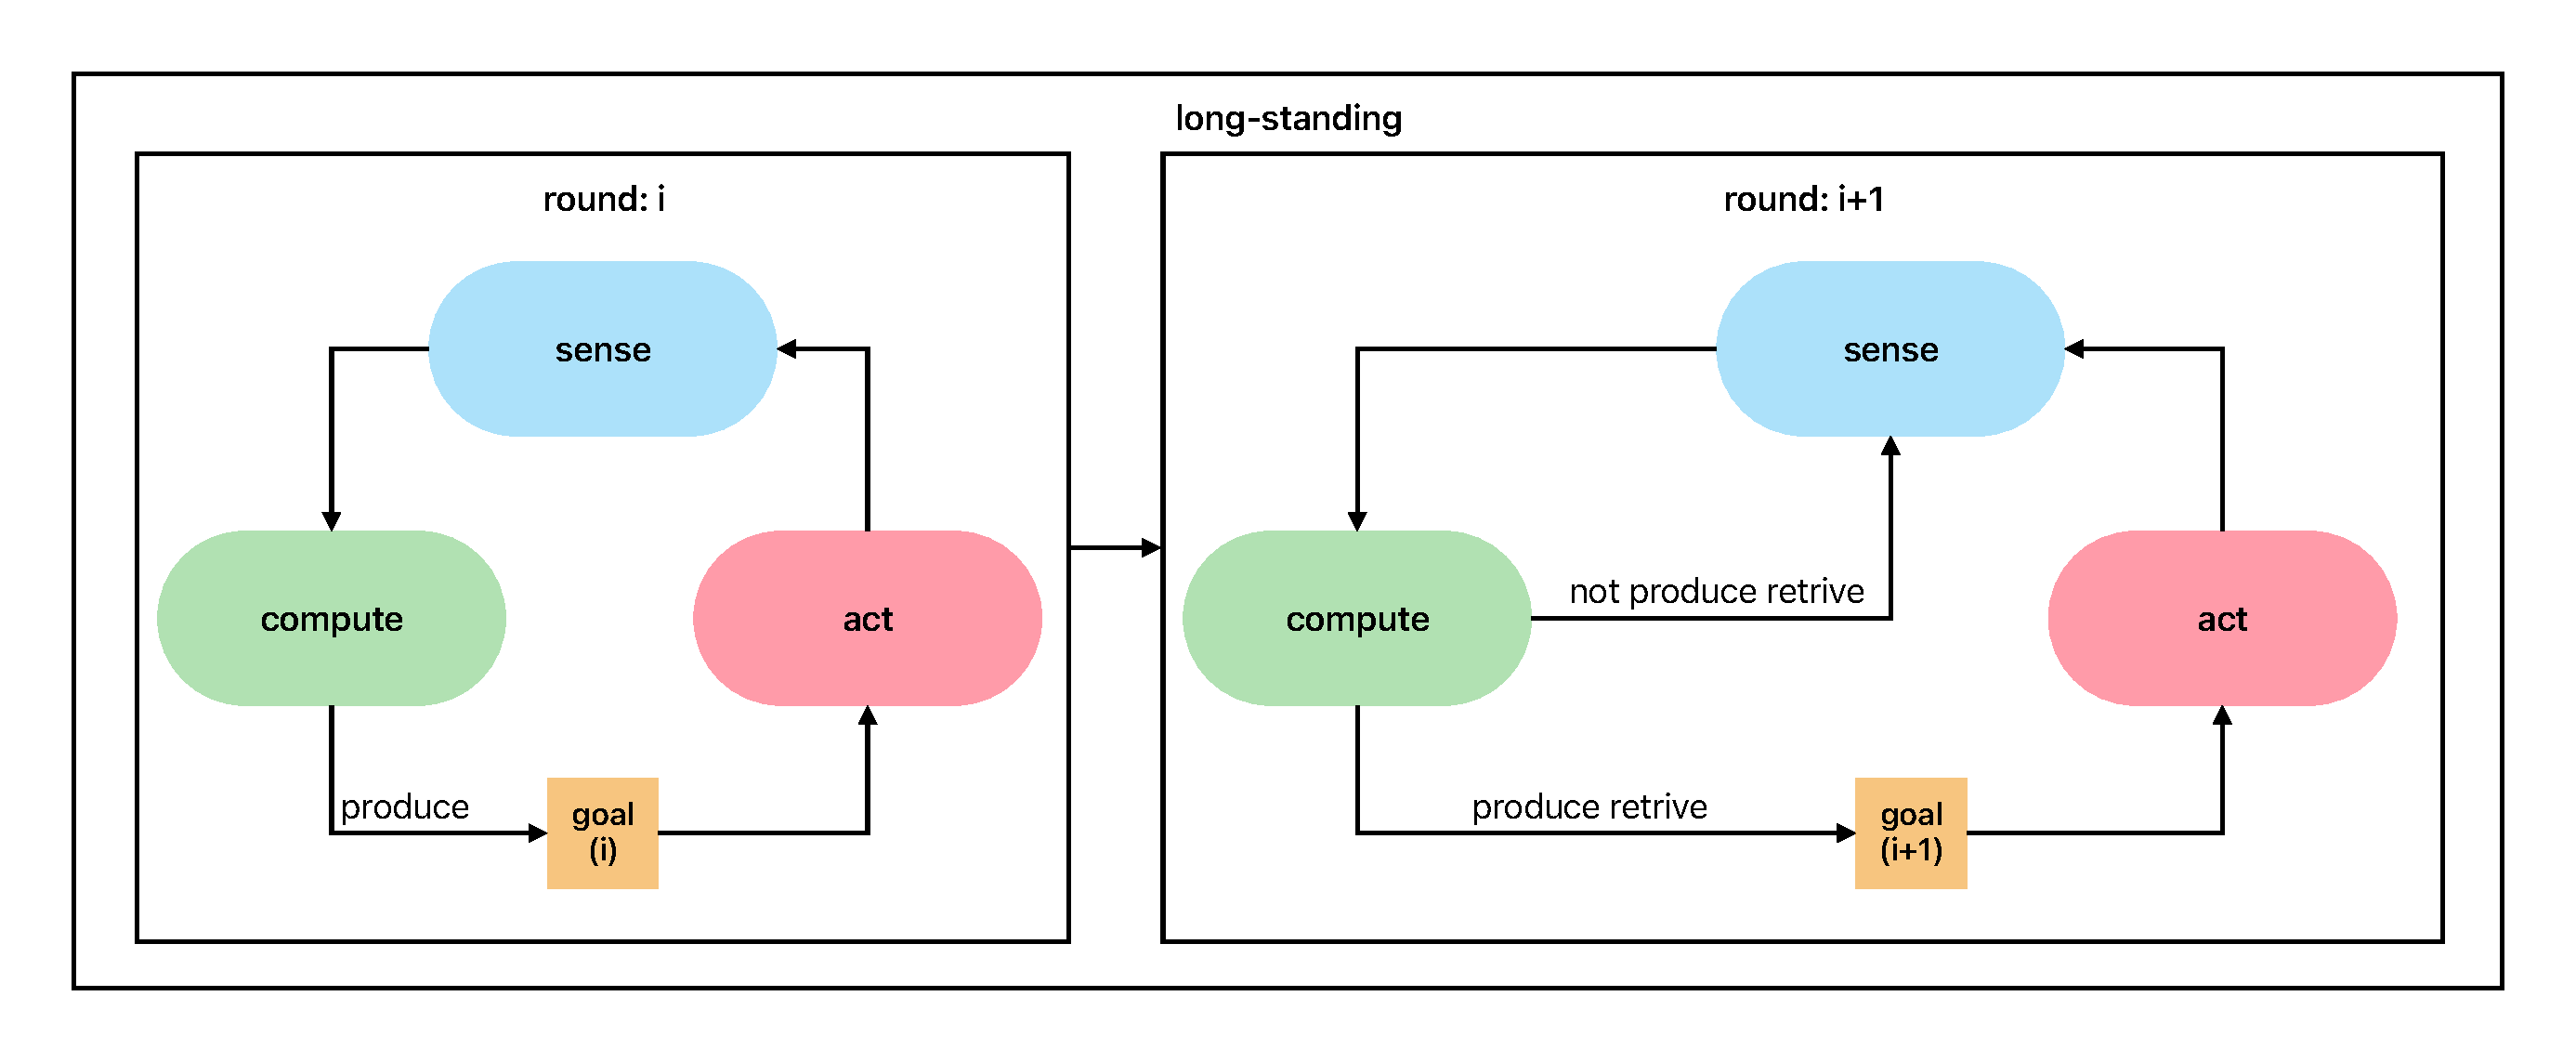
\includegraphics[width=.99\linewidth]{figures/long-standing.pdf}
    \caption{Modalità Long Standing}
    \label{fig:long-standong}
\end{figure}

Questo modello di attuazione è modellato come una funzione pura (sezione \ref{sec:fp} quindi priva di effetti collaterali. Se ci si trova in un contesto in cui l'esecuzione dell'attuazione richiede un certo tempo allora il progettista del sistema aggregato può andare a modellare il sistema in modo tale da tenere in considerazione questo aspetto.

Come è possibile vedere in figura \ref{fig:macro-swarm-int} \cite{Macroswarm} il framework è composto da diversi moduli che a loro volta contengono diversi blocchi, ognuno con un compito specifico, solo alcuni di questi blocchi sono sono stati utilizzati per la realizzazione del progetto e saranno descritti nei prossimi paragrafi.

\paragraph{Movements blocks} 
Questi blocchi si occupano di controllare i movimenti di ogni agente (dispositivo) della flotta. Il Movimento più semplice è descritto da un vettore \verb|Vector(x,y,z)| che rappresenta la direzione del movimento in uno spazio 3-dimensionale. 

\begin{lstlisting}[language=Scala, label={lst:vector-example}]
    Vector(3.6, 0, 0)
\end{lstlisting}

L'esempio \ref{lst:vector-example} rappresenta un movimento di $3.6 \frac{m}{s}$ lungo l'asse $x$. Una volta definito il blocco di movimento per un certo agente, i valori $x,y,z$ devono essere accuratamente mappati sui motori (attuatori più in generale) del dispositivo per ottenere il movimento desiderato. Procedere con una corretta mappatura è di fondamentale importanza quando si lavora su un sistema eterogeneo poiché si dovranno gestire dispositivi differenti equipaggiati da motori (attuatori) differenti.

Un'altro blocco ``semplice'' è \verb|brownian| che genera un vettore di movimento casuale ad ogni round, è possibile definire uno scalare (\verb|scale|) che rappresenta la velocità massima del movimento casuale.

Sono disponibili anche blocchi più complessi (\cref{lst:movement-module}), alcuni di questi simulati in figura \ref{fig:movement-simulations}:
\begin{itemize}
    \item \verb|goTo|: permette di definire un target (posizione assoluta) che gli agenti devono raggiungere
    \item \verb|explore|: definito uno spazio rettangolare con i valori \verb|minBound| e \verb|maxBound|, il blocco produce vettori da assegnare agli agenti per esplorare l'intero spazio
    \item \verb|maintainTrajectory|: permette di mantenere un certo vettore di movimento per un certo periodo di tempo
    \item \verb|maintainUntil|: permette di mantenere un certo vettore di movimento fino a quando non viene raggiunta una certa condizione
    \item \verb|obstacleAvoidance|: genera vettori di movimento da assegnare agli agenti per evitare ostacoli
\end{itemize}

In figura \ref{fig:movement-simulations} \cite{Macroswarm} sono state simulate le funzioni \verb|goTo|, \verb|explore| \\ e \verb|obstacleAvoidance| su Alchemist, un simulatore di sistemi aggregati.

\begin{figure}
    \centering
    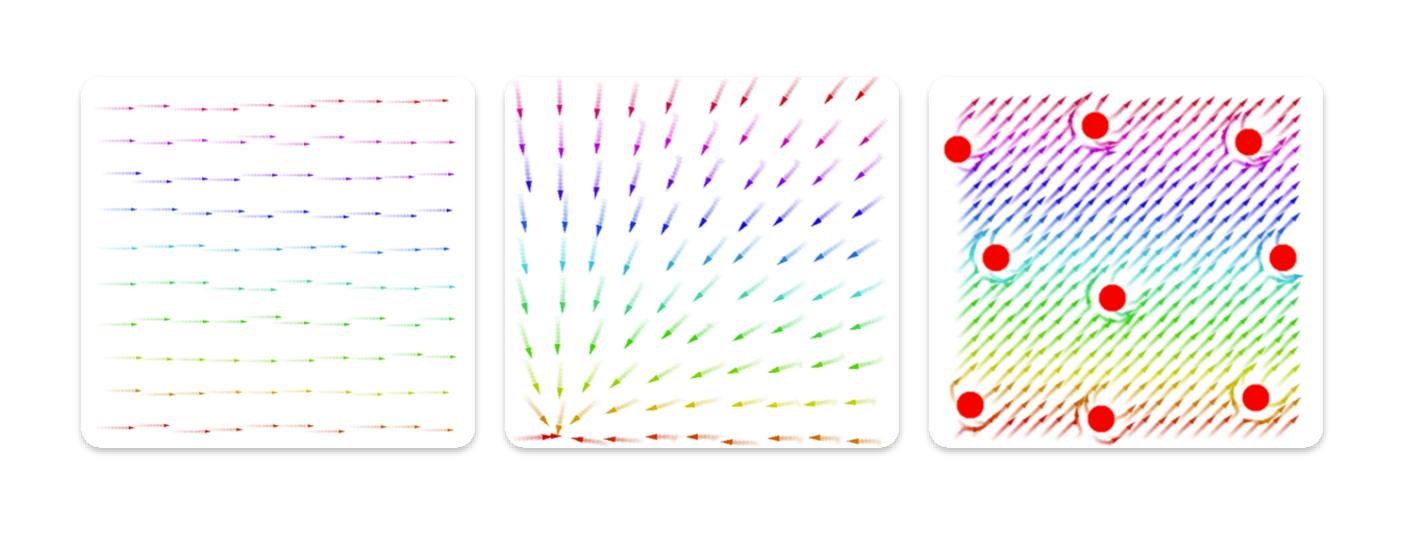
\includegraphics[width=.9\linewidth]{figures/movement-simulations.pdf}
    \caption{Simulazioni dei blocchi di movimento eseguita su Alchemist.}
    \label{fig:movement-simulations}
\end{figure}

\begin{lstlisting}[language=Scala, label={lst:movement-module}, caption={Funzioni del modulo di movimento}]
    // movimento casuale
    def brownian(scale: Double): Vector
    
    // posizioni assolute
    def goTo(target: Point3D): Vector
    def explore(minBound: Point3D, maxBound: Point3D): Vector

    // condizioni temporali
    def maintainTrajectory(trajectory: => Vector)(time: FiniteDuration):Vector

    // condizioni booleane
    def maintainUntil(direction: Vector)(condition: Boolean): Vector

    // elusione ostacoli
    def obstacleAvoidance(obstacles: List[Vector]): Vector
\end{lstlisting}

Questi blocchi possono essere assemblati per costruirne di nuovi più complessi, ad esempio, per creare un comportamento ``muovi fino a destinazione evitando gli ostacoli'' possiamo implementare un blocco nuovo nel seguente modo \cref{lst:complex-movement}:

\begin{lstlisting}[language=Scala, label={lst:complex-movement}, caption={Comportamento complesso}]
    def moveToTargetAvoidingObstacles(target: Point3D, obstacles: List[Vector]): Vector = {
        val targetMovement = goTo(target)
        val obstacleAvoidanceMovement = obstacleAvoidance(obstacles)
        (targetMovement + obstacleAvoidanceMovement).normalize
    }
\end{lstlisting}

La composizione di questi blocchi permette di creare comportamenti complessi in modo semplice e intuitivo andando semplicemente a sommare comportamenti più semplici. È importante andare a \textit{normalizzare} il risultato del comportamento complesso per produrre un singolo vettore nel caso in cui il movimento sia composto da più vettori.

\paragraph{Leader-based blocks} Per gestire un insieme di agenti in modo coordinato al fine di raggiungere un obiettivo si è valutato che ci fosse la necessità di avere un nodo leader che si occupasse di coordinare gli altri nodi, proprio come succede nella natura nel caso dei branchi. Il leader può essere scelto secondo un certo criterio (ad esempio per le sue caratteristiche speciali oppure per la sua posizione all'interno del gruppo) oppure casualmente ma è anche possibile andare a creare un leader \textit{virtuale}, che quindi non è realmente presente nel ambiente. Allo stato attuale sono presenti solo due blocchi ritenuti essenziali:
\begin{itemize}
    \item \verb|alignWithLeader|: permette di allineare la velocita degli agenti con quella del leader
    \item \verb|sinkAt|: permette di far convergere gli agenti verso il leader
\end{itemize} 

Nel caso si necessiti di avere un comportamento più complesso che porti alla nascita di sotto-team si possono utilizzare i blocchi presenti in \textbf{Team formation blocks} che non approfondiremo in questo contesto.

\paragraph{Pattern formation blocks}
Per creare comportamenti coordinati per un team al fine di raggiungere un task si possono usare i blocchi presenti in \textbf{Leader-based blocks} e \textbf{Team formation blocks}, nel caso invece si è interessati soltanto alla forma geometrica che il team deve assumere si possono usare i blocchi presenti in \textbf{Pattern formation blocks}. La seconda tipologia di blocchi è una derivazione della prima poiché necessita della identificazione di un leader, il leader si occupa di collezionare le distanze dei propri ``sottoposti'' per poi assegnare loro una certa direzione per raggiungere la formazione desiderata. Il leader utilizza il Gradient-cast ed i Collect-cast per raccogliere le informazioni e utilizza, nuovamente, Gradient-cast per assegnare le direzioni.

Allo stato attuale del framework è possibile costruire in modo semplice le seguenti figure geometriche:
\begin{itemize}
    \item formazione a ``V'', come quella dei volatili
    \item linea
    \item cerchio
\end{itemize}

Tutte e tre le formazioni in figura \ref{fig:formation-simulations} \cite{Macroswarm} si possono muovere nello spazio e necessitano di un leader. Nel caso il leader vada a variare la sua velocità di movimento i nodi vicini si adatteranno alla velocità del leader. Questo tipo di formazioni sono capaci di ricostruirsi anche nel caso cambi il numero di nodi oppure un fenomeno esterno vada a disturbarne la struttura.

\begin{figure}
    \centering
    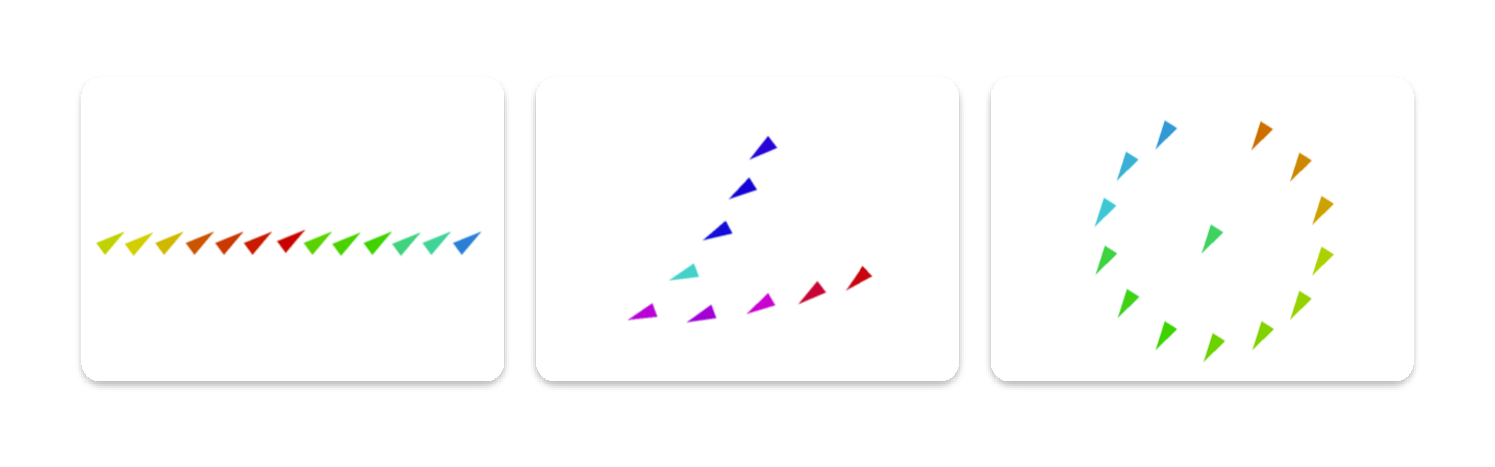
\includegraphics[width=.9\linewidth]{figures/formation-simulations.pdf}
    \caption{Simulazioni delle formazioni eseguite su Alchemist, in ordine: linea, formazione a V, cerchio.}
    \label{fig:formation-simulations}
\end{figure}

\section{Thymio e tdmclient}

\begin{quote}
    \raggedright
    ``Thymio è un robot educativo open-source progettato da ricercatori dell'EPFL (Politecnico federale di Losanna), in collaborazione con l'ECAL (Università d'arte e design di Losanna), e prodotto da Mobsya, un'associazione no-profit la cui missione è quella di offrire percorsi STEAM completi e coinvolgenti a studenti di tutte le età.''
    \begin{flushright}
        \textit{-- \href{https://www.thymio.org/}{Mobsya}}
    \end{flushright}
\end{quote}

\begin{figure}
    \centering
    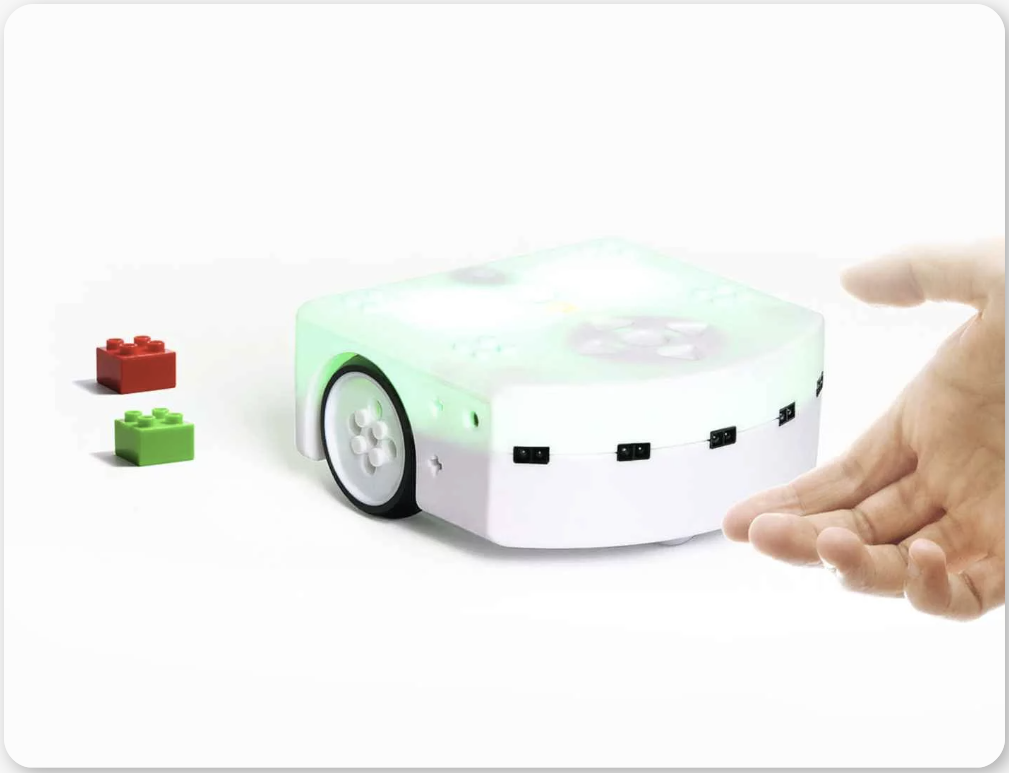
\includegraphics[width=.7\linewidth]{figures/thymio.png}
    \caption{Robot Thymio}
    \label{fig:thymio-robot}
\end{figure}

Thymio \cite{mobsyaThymioDevice} è un robot programmabile con un'ampia varietà di sensori e attuatori, tra cui:
\begin{itemize}
    \item 9 sensori a infrarossi (portata circa 10 cm)
    \item 5 pulsanti a sfioramento (tecnologia capacitiva)
    \item 1 accelerometro a tre assi
    \item 1 termometro
    \item 1 microfono
    \item 1 ricevitore a infrarossi per il telecomando
    \item 39 LED controllabili
    \item 2 motori DC collegati alle ruote
    \item 1 altoparlante
\end{itemize}

Il deploy del codice sul robot Thymio avviene tramite un radio dongle USB.
\paragraph{Thymio Network}: La connessione wireless dei robot è basata sul protocollo \href{https://en.wikipedia.org/wiki/IEEE_802.15.4}{802.15.4} in banda con frequenza 2.4 GHz \cite{wikidotSettingWireless}. Questo protocollo permette di gestire una rete con molti nodi a discapito del rispetto delle seguenti condizioni:

\begin{itemize}
    \item tutti i nodi devono trovarsi tutti nello stesso canale radio (sono disponibili 3 reti: [0, 1, 2])
    \item tutti i dispositivi devono avere lo stesso Identificativo di rete (PAN ID)
    \item tutti devono avere un nodo Identificativo univo (nodeID)
\end{itemize}

Il protocollo è stato implementato in modo da permettere la comunicazione tra i robot e con il computer tramite il dongle USB.

Il dispositivo è stato scelto per essere implementato nella demo per la notte dei ricercatori 2024 in quanto si tratta di un robot molto versatile e adatto a molteplici applicazioni. Inoltre, il robot è molto diffuso nelle scuole e nei laboratori di robotica educativa, quindi è un'ottima scelta per mostrare il potenziale di ScaFi in un contesto educativo.

Questo piccolo robot nasce per essere programmato con linguaggi a blocchi come VPL, VPL3, Scratch, Blocky e non come Aseba, Python e Ros, tutti accessibili dalla suite dedicata \textit{``Thymio Suite''} \cite{mobsyaThymioDevice}.

Noi ci concentreremo sull'uso di Python. 

Python a differenza di altri linguaggi (ad esempio C/C++) è interpretato e non compilato. I linguaggi compilati prevedono la conversione del programma scritto in un linguaggio ad alto livello in linguaggio macchina per poi farlo eseguire dal processore, occorre quindi compilare il sorgente ad ogni nuova modifica per poi re-eseguirlo. In Python, invece, il codice sorgente viene eseguito direttamente dal programma interprete, il quale esegue ogni comando riga per riga \cite{robotadvanceUsingEducational}.

\begin{figure}
    \centering
    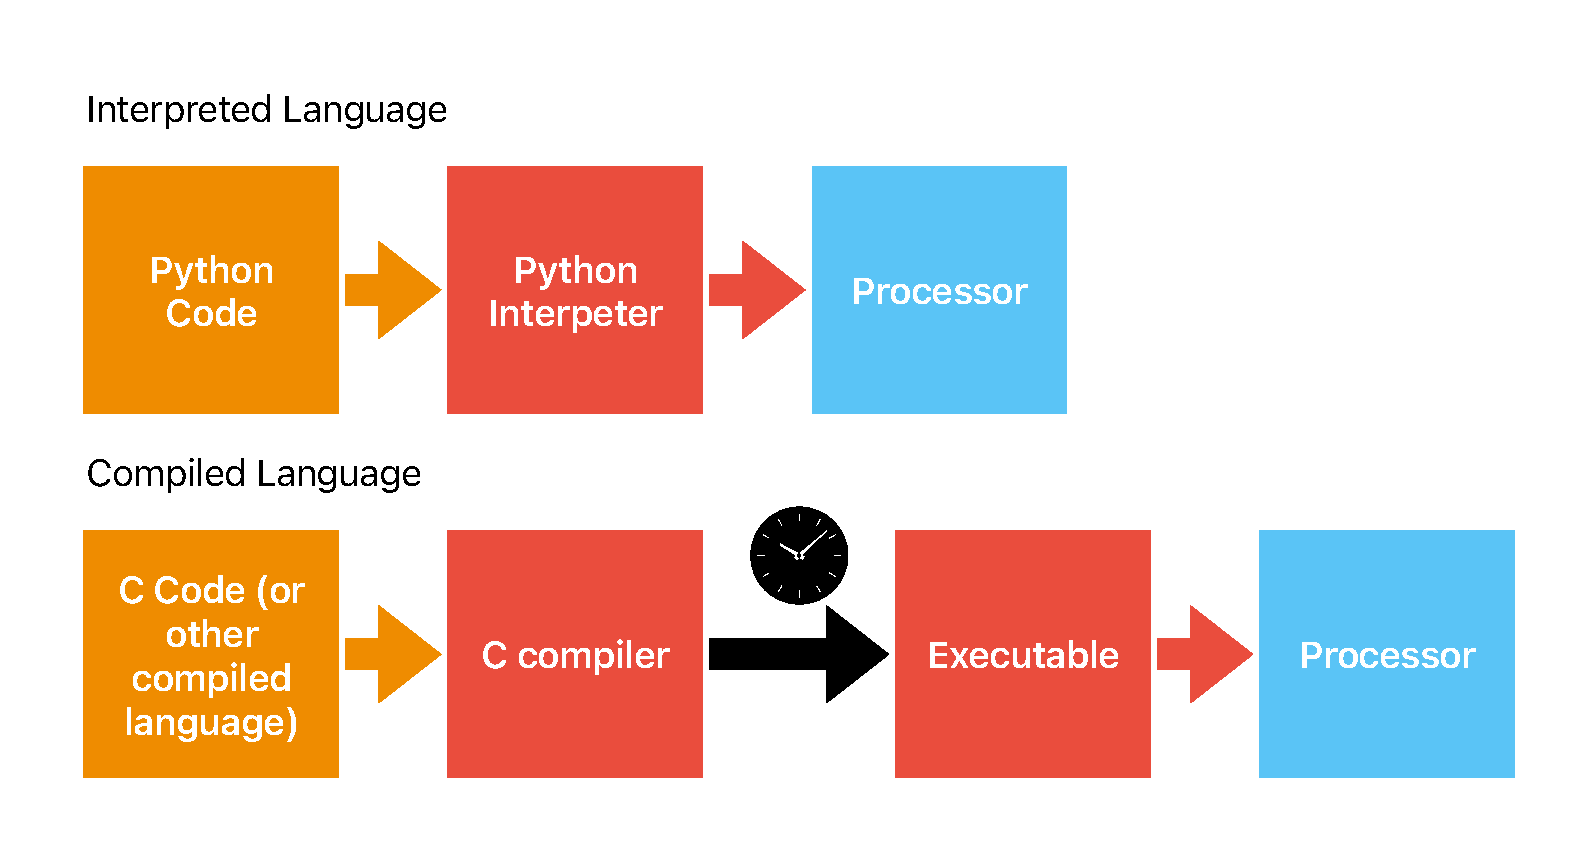
\includegraphics[width=.8\linewidth]{figures/interpreter-compiler.pdf}
    \caption{Interprete vs Compilatore}
    \label{fig:interpreter-vs-compiler}
\end{figure}

Nel caso del robot Thymio, non è presente un interprete nel suo microcontrollore. È presente, invece, una Aseba Virtual Machine che permette di eseguire programmi scritti in linguaggio Aseba. 

Aseba è un linguaggio di programmazione ad alto livello basato su architettura ad eventi, il che significa che gli eventi sono eseguiti in modo asincrono. Gli eventi sono identificati da un Identificativo ed opzionalmente da un \textit{payload} (dati aggiuntivi). 
Gli eventi possono essere di due tipi:
\begin{itemize}
    \item \textbf{global events}: eventi generati dai nodi e condivisi con la rete
    \item \textbf{local events}: eventi generati da un nodo e non condivisi con la rete (ad esempio un evento generato da un sensore dello stesso nodo)
\end{itemize}

Un esempio di codice Aseba è il seguente \cref{lst:aseba-code}.
% Non è disponibile Aseba quindi useremo Python
\begin{lstlisting}[language=Python, label={lst:aseba-code}, caption={Esempio di codice Aseba con eventi}]
    var state

    callsub init  # Inizializza il programma

    sub init
        state = 0
        call leds.bottom.left(0,0,32)
        call leds.bottom.right(0,32,0)
        call leds.top(32,0,0)

    # Re-inizia quando il pulsante centrale viene premuto
    onevent button.center
        callsub init
\end{lstlisting}

Il \textbf{Thymio Device Manager} è una delle feature della Thymio Suite, si occupa di gestire la rete dei Thymio. Inoltre ha il compito di tradurre il sorgente, scritto dall'utente, da linguaggio Aseba ad Aseba bytecode per poi eseguire il \textit{deploy} sul robot. Per l'utilizzo di Python, invece, è necessario l'utilizzo del modulo \textbf{tdmclient} che si occupa di far comunicare Python con il \ac{TDM} (figura \ref{fig:tdmclient}) \cite{pypiTdmclient}. È necessario che la Thymio Suite sia in esecuzione per poter utilizzare il modulo \textbf{tdmclient}, il quale, a sua volta, necessita dell'utilizzo di \textbf{Python 3} come interprete.

Questo modulo permette di:
\begin{itemize}
    \item accedere alle variabili, sensori, attuatori del robot
    \item convertire uno script Python in un script Aseba (transpiler)
    \item inviare codice Aseba al \ac{TDM} che a sua volta invia il relativo bytecode al  robot Thymio 
\end{itemize}

\begin{figure}
    \centering
    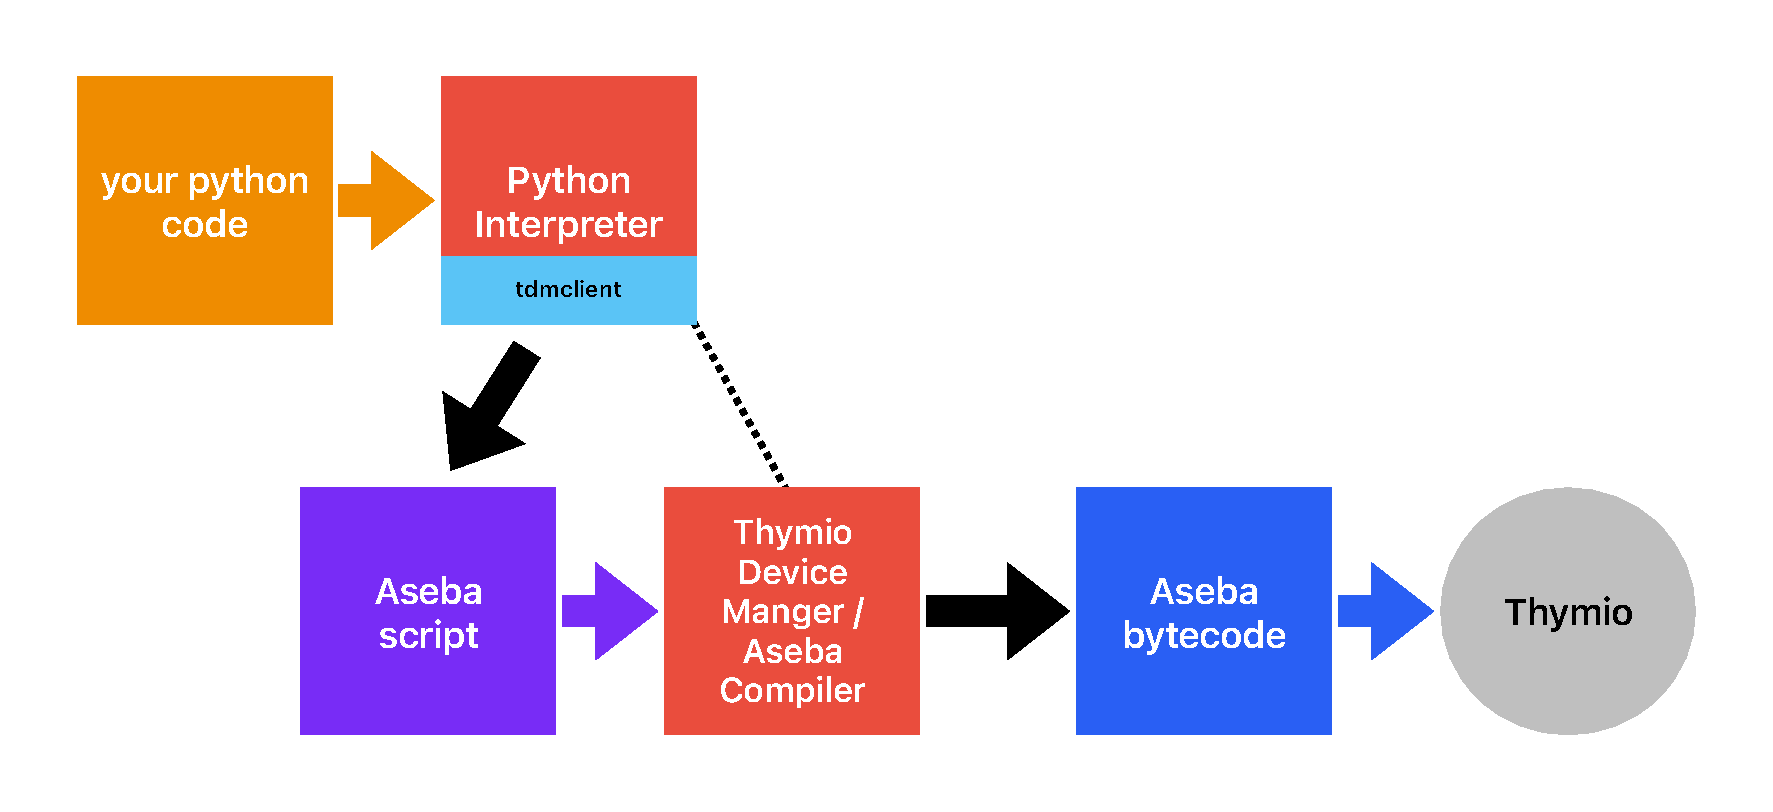
\includegraphics[width=.8\linewidth]{figures/TDM.pdf}
    \caption{Tdmclient workflow}
    \label{fig:tdmclient}
\end{figure}

Le possibilità offerte da questo modulo sono molteplici, ad esempio è possibile inviare comandi direttamente ad un robot Thymio da terminale:

\begin{lstlisting}[language=Bash, label={lst:command-to-thymio}, caption={Esempio di invio di comando (foo) ad un robot Thymio}]
    python3 -m tdmclient sendevent --event foo --data 123
\end{lstlisting}

In \cref{lst:command-to-thymio} si assume che il robot accetti un evento di nome \textit{foo} con un payload di tipo intero e che il robot sia in ascolto di eventi (\textit{unlocked}). Per metter in ascolto un robot di un certo evento è necessario andare ad inserire una vista su quel determinato robot dalla Thymio Suite.

\begin{lstlisting}[language=Python, label={lst:thymio-catch-event}, caption={Esempio di programma interno a Thymio per la ricezione di eventi (foo)}]
    var x

    onevent foo
        x = event.args[0]
\end{lstlisting}

Il modulo permette di eseguire il transpile (conversione) di un programma Python in Aseba. Per farlo è necessario utilizzare il comando \textit{transpile} del modulo \textbf{tdmclient}:

\begin{lstlisting}[language=Bash, label={lst:transpile-python-to-aseba}, caption={Esempio di transpile di un programma Python (print.py) in Aseba}]
    python3 -m tdmclient transpile examples/print.py
\end{lstlisting}

Utilizzando il modulo aggiuntivo \verb|ClientAsync| è possibile modificare le variabili dei robot Thymio attraverso chiamate asincrone in uno script \textbf{Python}.
Si andrà ad esaminare ulteriormente questa feature di \textbf{tdmclient} nel capitolo \ref{chap:design} e \ref{chap:implementazione} poiché è ciò che si è utilizzato per la progettazione del nostro sistema.

\section{Aruco Tag}

Gli Aruco marker sono tag quadrati che possono essere rilevati da una camera. Ogni tag è una matrice $4 \times 4$ ed ha un codice (intero) univoco associato che può essere rilevato da un algoritmo di visione artificiale come in figura \ref{fig:aruco-markers} \cite{opencvOpenCVDetection}. È rilevante notare che la matrice di ogni Aruco marker corrisponde ad uno stesso codice per ogni sua versione trasposta. 
Questi tag sono molto utili per la localizzazione e la navigazione di robot autonomi. Sarà questo strumento che verrà utilizzato per la demo della notte dei ricercatori per la localizzazione e calcolo della direzione dei robot Thymio.

\begin{figure}
    \centering
    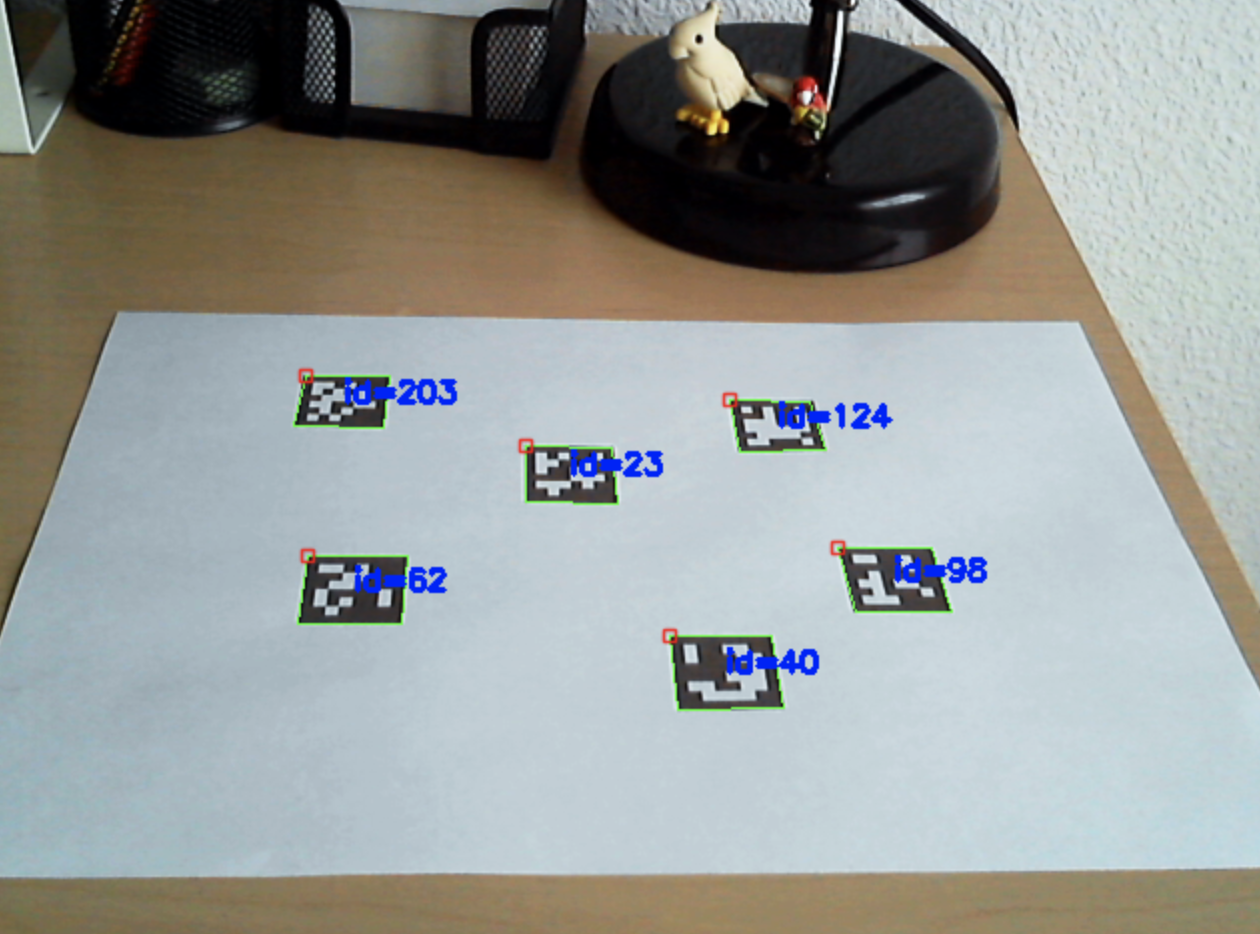
\includegraphics[width=.8\linewidth]{figures/aruco-markers.png}
    \caption{Aruco markers identificati da un algoritmo di visione artificiale}
    \label{fig:aruco-markers}
\end{figure}

Questo strumento è già presente nel sistema in questione.

%----------------------------------------------------------------------------------------
\chapter{Analisi}
\label{chap:analisi}
%----------------------------------------------------------------------------------------

\section{Obiettivi}
Il progetto \href{https://github.com/cric96/researcher-night-demo.git}{``researcher-night-demo''} è nato per dimostrare, attraverso simulazioni in ambiente reale, le potenzialità di ScaFi. L'obiettivo di questo progetto è dimostrare l'eterogeneità di questo tipo di sistemi andando ad estendere ai robot già implementati il supporto per un nuovo modello di robot (Thymio in figura \ref{fig:thymio-robot}. ) e andando a gestire gli eventuali vincoli di compatibilità.

Inizialmente, la demo, presentava soltanto la possibilità di utilizzare i robot Wave (figura \ref{fig:wave-robot}). I Wave sono robot equipaggiati da 4 ruote motrici (4WD), scocca d'acciaio ed un modulo ESP32 (microcontrollore programmabile) già implementato di software (open-source) che ne permette il controllo mezzo protocollo WiFi o Bluetooth.

\begin{figure}
    \centering
    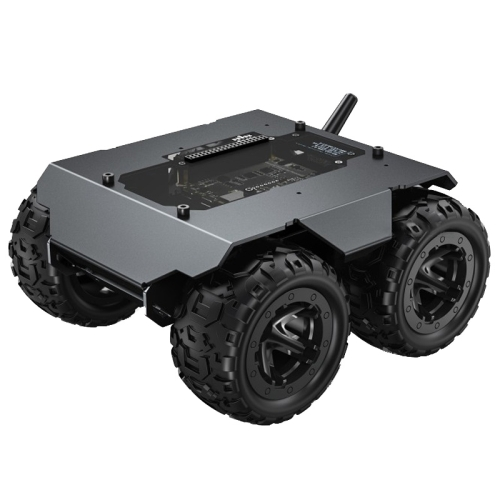
\includegraphics[width=.3\linewidth]{figures/wave-robot.jpg}
    \caption{Robot Wave}
    \label{fig:wave-robot}
\end{figure}

A livello strutturale il sistema è caratterizzato da un Environment che rappresenta il mondo in cui gli agenti si muovono e raccolgono dati mediante Sensori, un EnvironmentProvider che si occupa di carpire le informazioni utili sugli agenti e sull'Environment per fornirle al programma aggregato, programma aggregato che computa le informazioni ricevute dal EnvironmentProvider ed elabora il comportamento più performante per raggiungere l'obiettivo definito ed in fine un sistema di Attuazione che trasforma il comportamento definito dal programma aggregato in azioni che producono un effetto nel mondo reale (figura \ref{fig:uml}).

\begin{figure}
    \centering
    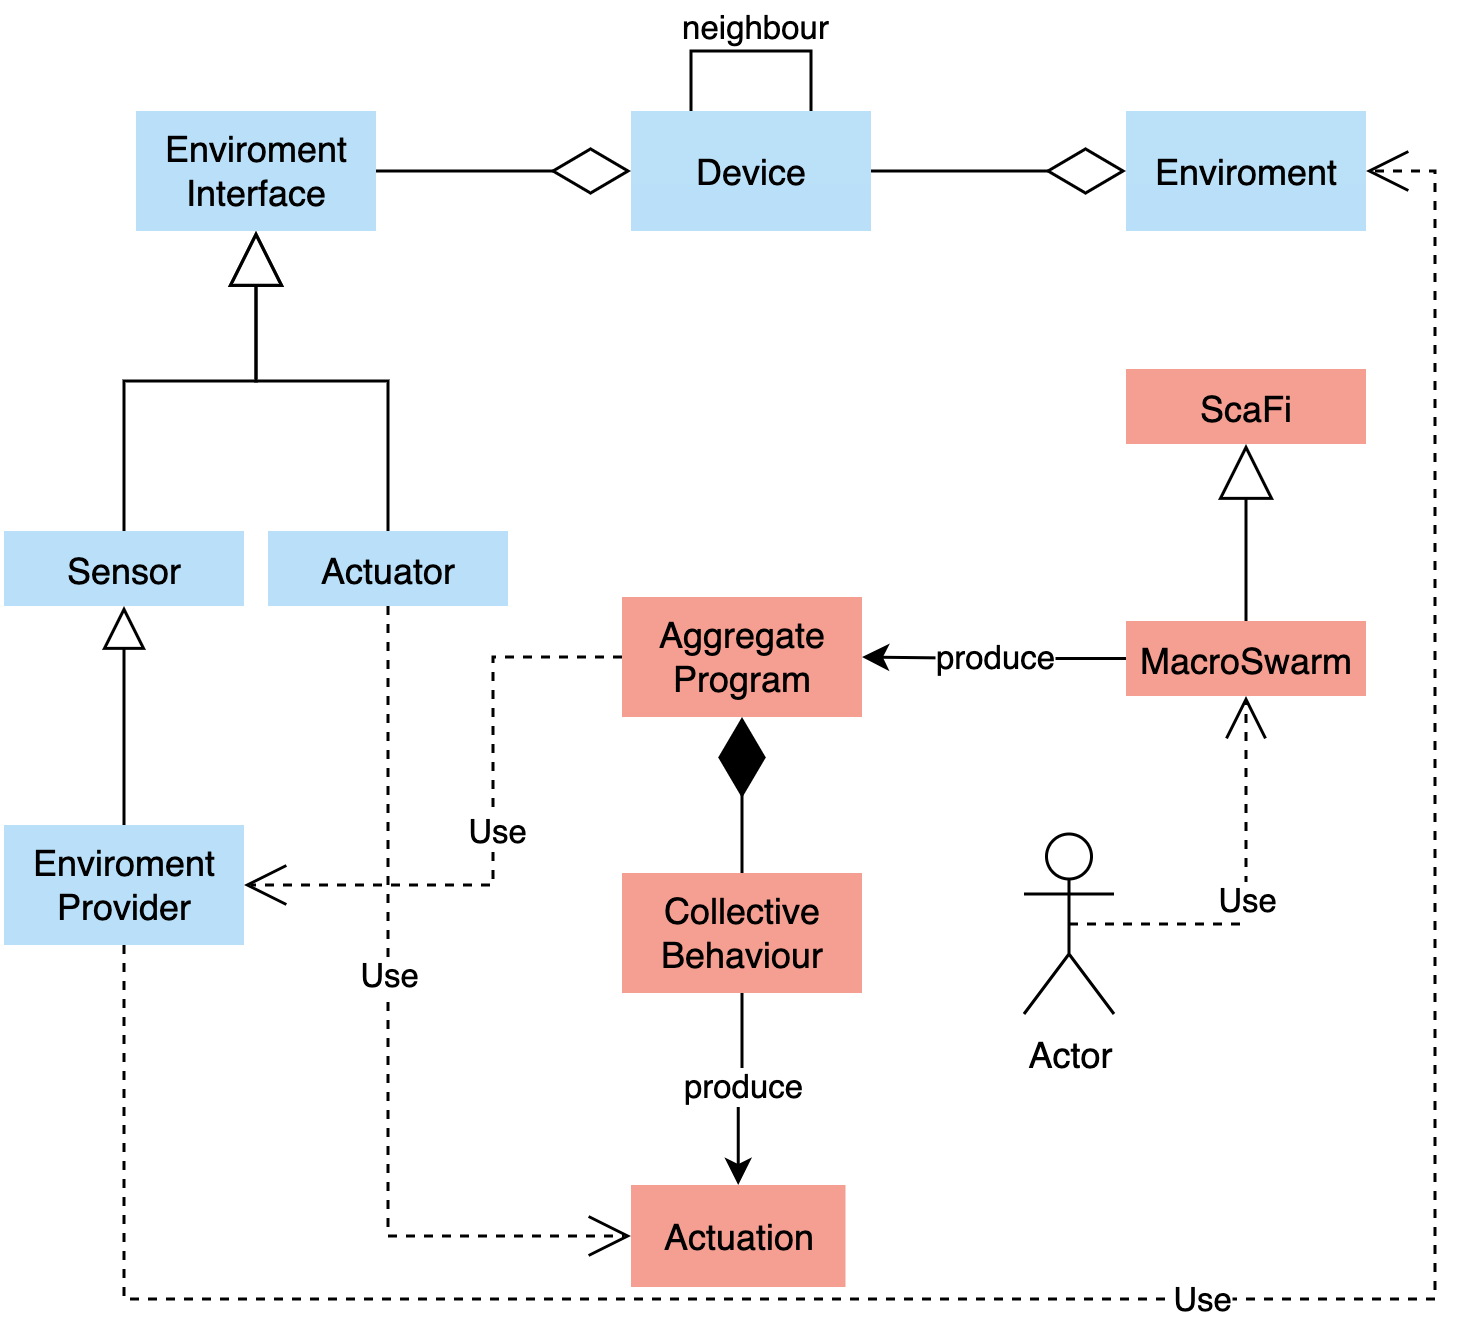
\includegraphics[width=.8\linewidth]{figures/uml.png}
    \caption{UML del sistema}
    \label{fig:uml}
\end{figure}

\section{Requisiti}

Requisiti funzionali:
\begin{itemize}
    \item Il sistema è progettato per l'utilizzo di grandi quantità di dispositivi eterogenei quindi si ritiene necessario che vengano caricati attraverso file di configurazione invece che essere definiti direttamente nel codice. Questo permette di avere un sistema più flessibile e facilmente estendibile.
    \item Integrare robot Thymio nel sistema già esistente.
\end{itemize}

Requisiti non funzionali:
\begin{itemize}
    \item Velocità nelle comunicazioni con i nuovi robot integrati.
\end{itemize}

%----------------------------------------------------------------------------------------
\chapter{Design}
\label{chap:design}
%----------------------------------------------------------------------------------------

A seguito di un analisi delle caratteristiche dei robot Thymio e dei protocolli di comunicazione che esso mette a disposizione si è optato per l'utilizzo del modulo \textbf{tdmclient} nel contesto di un server sviluppato utilizzando il framework Flask. Questo framework è stato sviluppato per la creazione di applicazioni web e, in particolare, per la creazione di \textit{API RESTful}\footnote{Le API sono l'interfaccia che utilizzano due o più sistemi informatici per lo scambio sicuro di informazioni. REST è un'architettura software sulla quale si possono progettare le API} da utilizzare per la comunicazione tra il server e il client che esegue il programma aggregato. 

Si è valutato anche l'utilizzo della libreria ScalaPy, che permette di sfruttare i moduli Python all'interno di un programma Scala, per incorporare le funzionalità di tdmclient direttamente all'interno del sistema aggregato ma data la ``non stabilità'' del progettato ScalaPy si è deciso di non impiegare questa soluzione.

In figura \ref{fig:classi} è possibile vedere l'architettura dell'intero sistema con le classi principali che lo compongono. Definito un ambiente \verb|DemoEnvironment| lo si popola di agenti che nel nostro contesto sono \verb|Robot| (che a loro volta possono essere di tipo \verb|Wave| o \verb|Thymio|). Il \verb|DemoEnvironment| è in grado di fornire le informazioni necessarie al \verb|AggregateOrchestrator| che, a sua volta, computa le informazioni ricevute e produce le attuazioni da eseguire \verb|RobotUpdate|. Queste attuazioni vengono decodificate dai \verb|Robot| che le trasformano in effetti tangibili nel mondo reale. Per permettere all'orchestratore di definire i comportamenti più adatti è necessario definire un \verb|EnvironmentProvider| che si occupa di fornire le informazioni necessarie. Nel nostro caso si tratta di una (tele) \verb|Camera|.

\begin{figure}
    \centering
    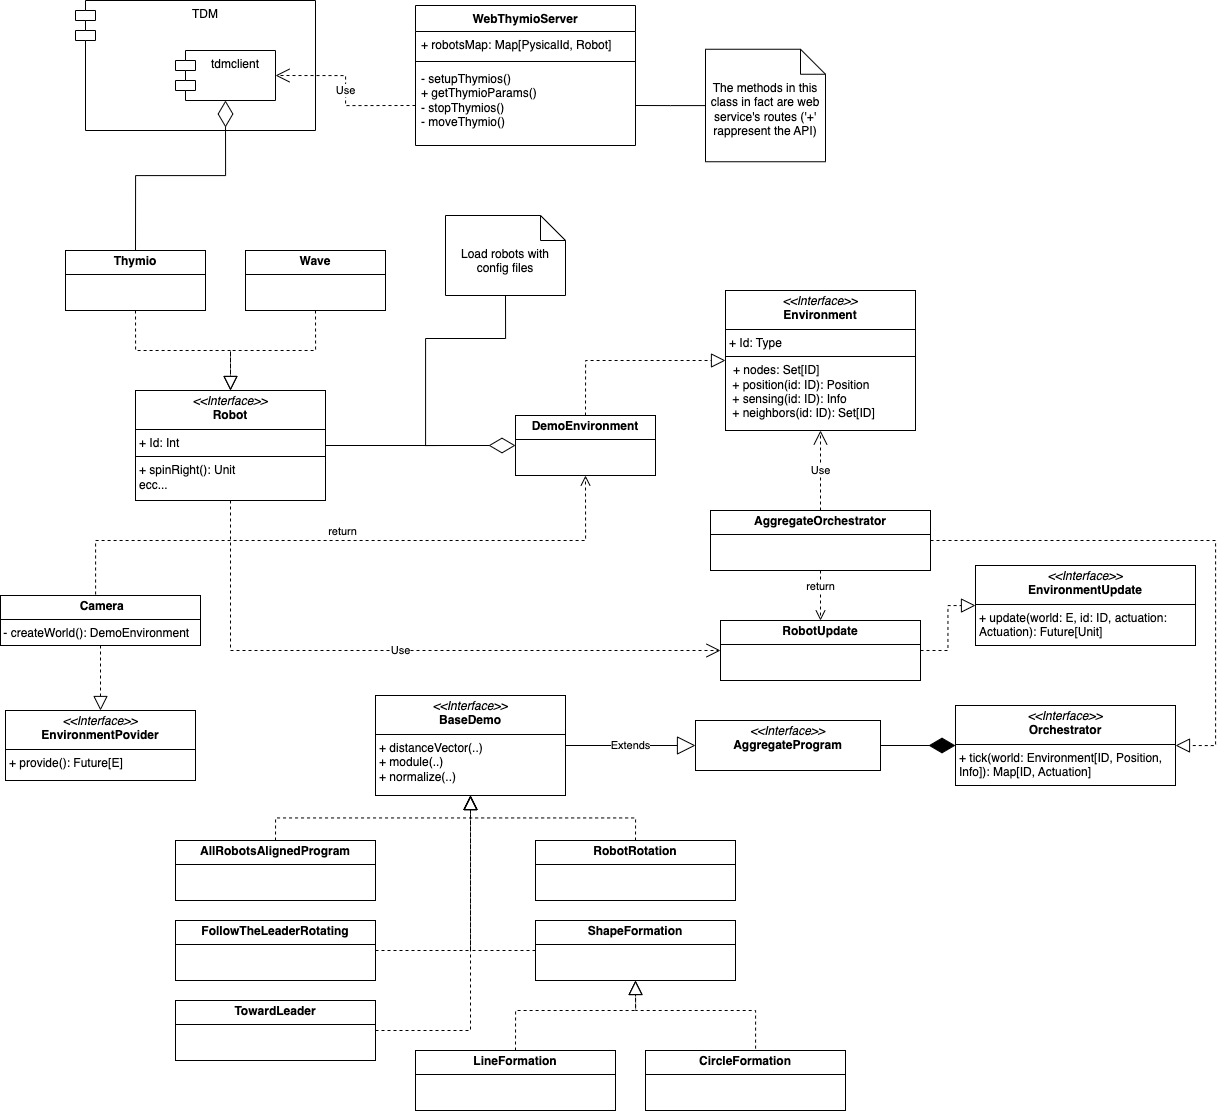
\includegraphics[width=.99\linewidth]{figures/classi.jpg}
    \caption{Diagramma delle classi}
    \label{fig:classi}
\end{figure}

\section{Architettura server Flask}

Il server sviluppato si occupa di gestire la comunicazione con due client come in figura \ref{fig:server-arc}:
\begin{itemize}
    \item il client Thymio Device Manager (TDM) che comunica con i robot Thymio
    \item il client che ospita ed esegue il programma aggregato
\end{itemize}

\begin{figure}
    \centering
    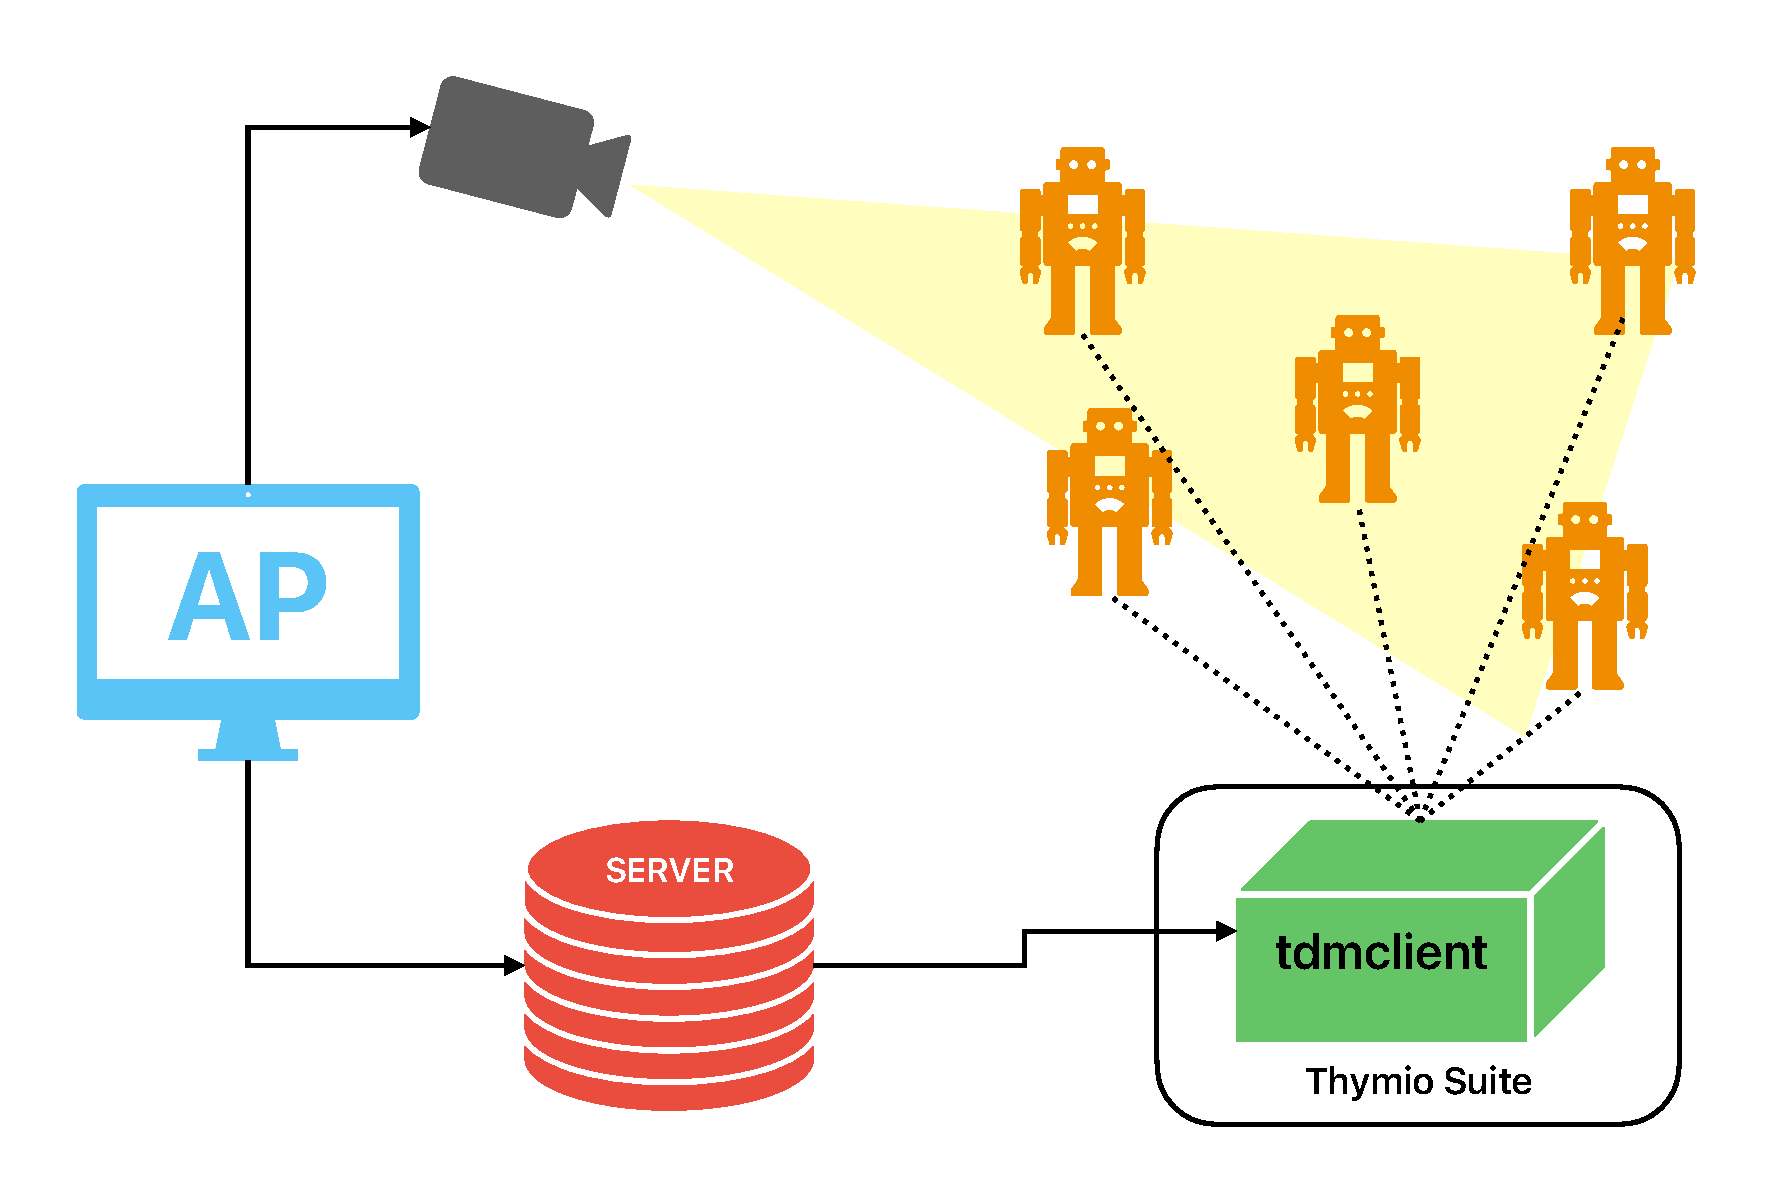
\includegraphics[width=.8\linewidth]{figures/server-arc.pdf}
    \caption{Design ad alto livello della soluzione proposta con l'implementazione del server Flask}
    \label{fig:server-arc}
\end{figure}

Il programma aggregato al fine di completare il task invia comandi per ogni Thymio al server Flask che, attraverso il modulo \textbf{tdmclient} si occupa di eseguire le attuazioni richieste. In figura \ref{fig:sequence} è possibile comprendere meglio il flusso di comunicazione tra i vari componenti del sistema. 

\begin{figure}
    \centering
    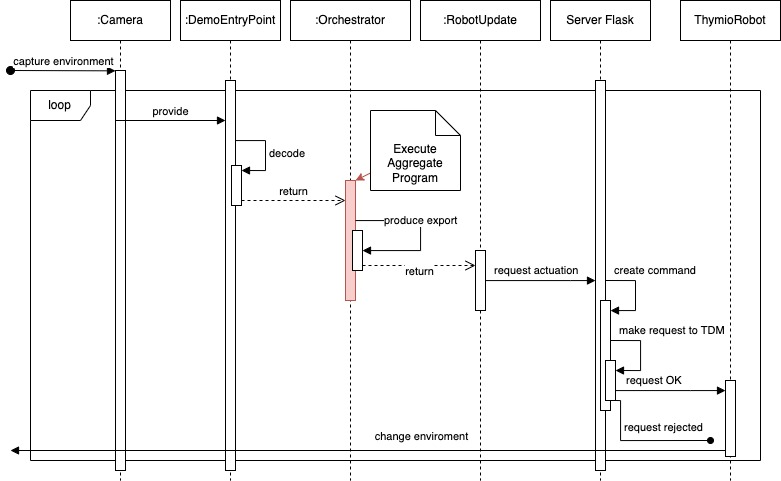
\includegraphics[width=.99\linewidth,angle=90]{figures/sequence.jpg}
    \caption{Diagramma di sequenza delle comunicazioni per il controllo dei Thymio Robot}
    \label{fig:sequence}
\end{figure}

%----------------------------------------------------------------------------------------
\chapter{Implementazione}
\label{chap:implementazione}
%----------------------------------------------------------------------------------------

Il progetto è stato sviluppato in linguaggio Scala ed è formato da tre componenti fisiche fondamentali:
\begin{itemize}
    \item webcam per il tracciamento dei Aruco Tag posizionati sopra ai robot
    \item macchina che esegue il sistema aggregato e che comunica con i robot, solitamente un computer
    \item collettivo di robot
\end{itemize}

La struttura del progetto si basa sul principio di Macroswarm, posizionandosi ad un livello di astrazione abbastanza alto da nascondere i dettagli implementativi dei dispositivi che si vuole andare a controllare. Di seguito una breve descrizione delle componenti principali del progetto:

\paragraph{Tracciamento robot}.
Per il tracciamento dei robot attraverso la webcam è stato sviluppato un applicativo Java di visione artificiale che rileva i tag Aruco e ne calcola la posizione e l'orientamento.

\paragraph{Core}. 
Il core del sistema è basato su ScaFi.
Per costruire i sistemi aggregati si utilizza la classe \verb|AggregateIncarnation| \cref{lst:agg-inc} che serve a poter definire i diversi programmi aggregati.

\begin{lstlisting}[language=Scala, label={lst:agg-inc}, caption={Classe AggregateIncarnation}]
    import it.unibo.scafi.incarnations.BasicAbstractIncarnation

    object AggregateIncarnation extends BasicAbstractIncarnation with BuildingBlocks
\end{lstlisting}

L'interfaccia \verb|Environment|\cref{lst:enviroment} rappresenta l'astrazione del mondo, essa rappresenta lo stato del mondo in un dato istante e va definita in base al contesto.

\begin{lstlisting}[language=Scala, label={lst:enviroment}, caption={Interfaccia Enviroment}]
    trait Environment[ID, Position, Info]:
        def nodes: Set[ID] // insieme di nodi definiti dagli identificatori ID
        def position(id: ID): Position // posizione di un certo nodo
        def sensing(id: ID): Info // le informazioni che un certo nodo espone
        def neighbors(id: ID): Set[ID] // vicinato di un certo nodo
\end{lstlisting}

La classe \verb|AggregateOrchestrator| è la componente principale del sistema poiché si occupa di leggere lo stato del mondo e ritornare l'attuazione da eseguire (export) per ogni agente.

\paragraph{Demo}
In demo si trova la reale implementazione del sistema aggregato che produce le attuazioni nel mondo reale a partire dalla definizione del ambiente in cui si lavora\cref{lst:demo-env}.

\begin{lstlisting}[language=Scala, label={lst:demo-env}, caption={Definizione dell'ambiente}]
    import it.unibo.core.DistanceEstimator.distance
    import it.unibo.core.Environment
    import it.unibo.demo.{ID, Info}
    import it.unibo.utils.Position.{Position, *, given}

    class DemoEnvironment(data: Map[ID, (Position, Info)], neighboursRadius: Double)
        extends Environment[ID, Position, Info]:

    override def nodes: Set[ID] = data.keySet

    override def position(id: ID): (Double, Double) = data(id)._1

    override def sensing(id: ID): Info = data(id)._2

    override def neighbors(id: ID): Set[ID] =
        data.filter { case (k, v) => data(id)._1.distance(v._1) <= neighboursRadius }.keys.toSet
\end{lstlisting}

\paragraph{Mock}
Il progetto dispone anche di uno spazio per testare programmi aggregati in un ambiente simulato implementato utilizzando la libreria \verb|JavaFX|. Questo ambiente permette di vedere i nodi della rete e le connessioni tra di essi.

\section{Implementazione del server Flask}

Lato Server, sono di rilevanza le implementazioni per rilevare i robot Thymio nella rete \cref{lst:setup-thymios} e per ricevere, attraverso l'API \cref{lst:api} i comandi per controllarli \cref{lst:command-to-thymio}.

\lstinputlisting[language=Python,label={lst:setup-thymios},caption={Funzione di setup per rilevare i Thymio nella rete}]{listings/getTymios.py}

L'API è stata costruita sotto forma di richiesta HTTP (GET) con parametro un JSON contente l'identificato fisico univoco del Thymio, la potenza da erogare nel motore sinistro e destro (nel caso la potenza sia negativa il motore andrà in senso inverso) \cref{lst:api}.

Nel sorgente è possibile notare che il server è sviluppato per essere eseguito nella stessa macchina che ospita il programma aggregato, attuale è eseguito in hardcoded sulla porta \verb|52000| di \textit{localhost}.

\lstinputlisting[language=php,label={lst:api},caption={API per il controllo dei Thymio}]{listings/api.url}

\lstinputlisting[language=Python,label={lst:move-thymios},caption={Implementazione API per inivare un comando di movimento al Thymio}]{listings/moveThymio.py}

Per completezza è stato sviluppata una semplice interfaccia web per poter inviare i comandi ai robot Thymio presentata in figura \ref{fig:web-interface}. È possibile utilizzarla per verificare che tutti i robot siano correttamente connessi alla rete mediante l'invio di comandi per il movimento e andare a fermarli tutti in caso di necessità.

È presente anche un pulsante per fermare tutti i robot nella rete nel caso si verifichi un'anomalia.

\begin{figure}
    \centering
    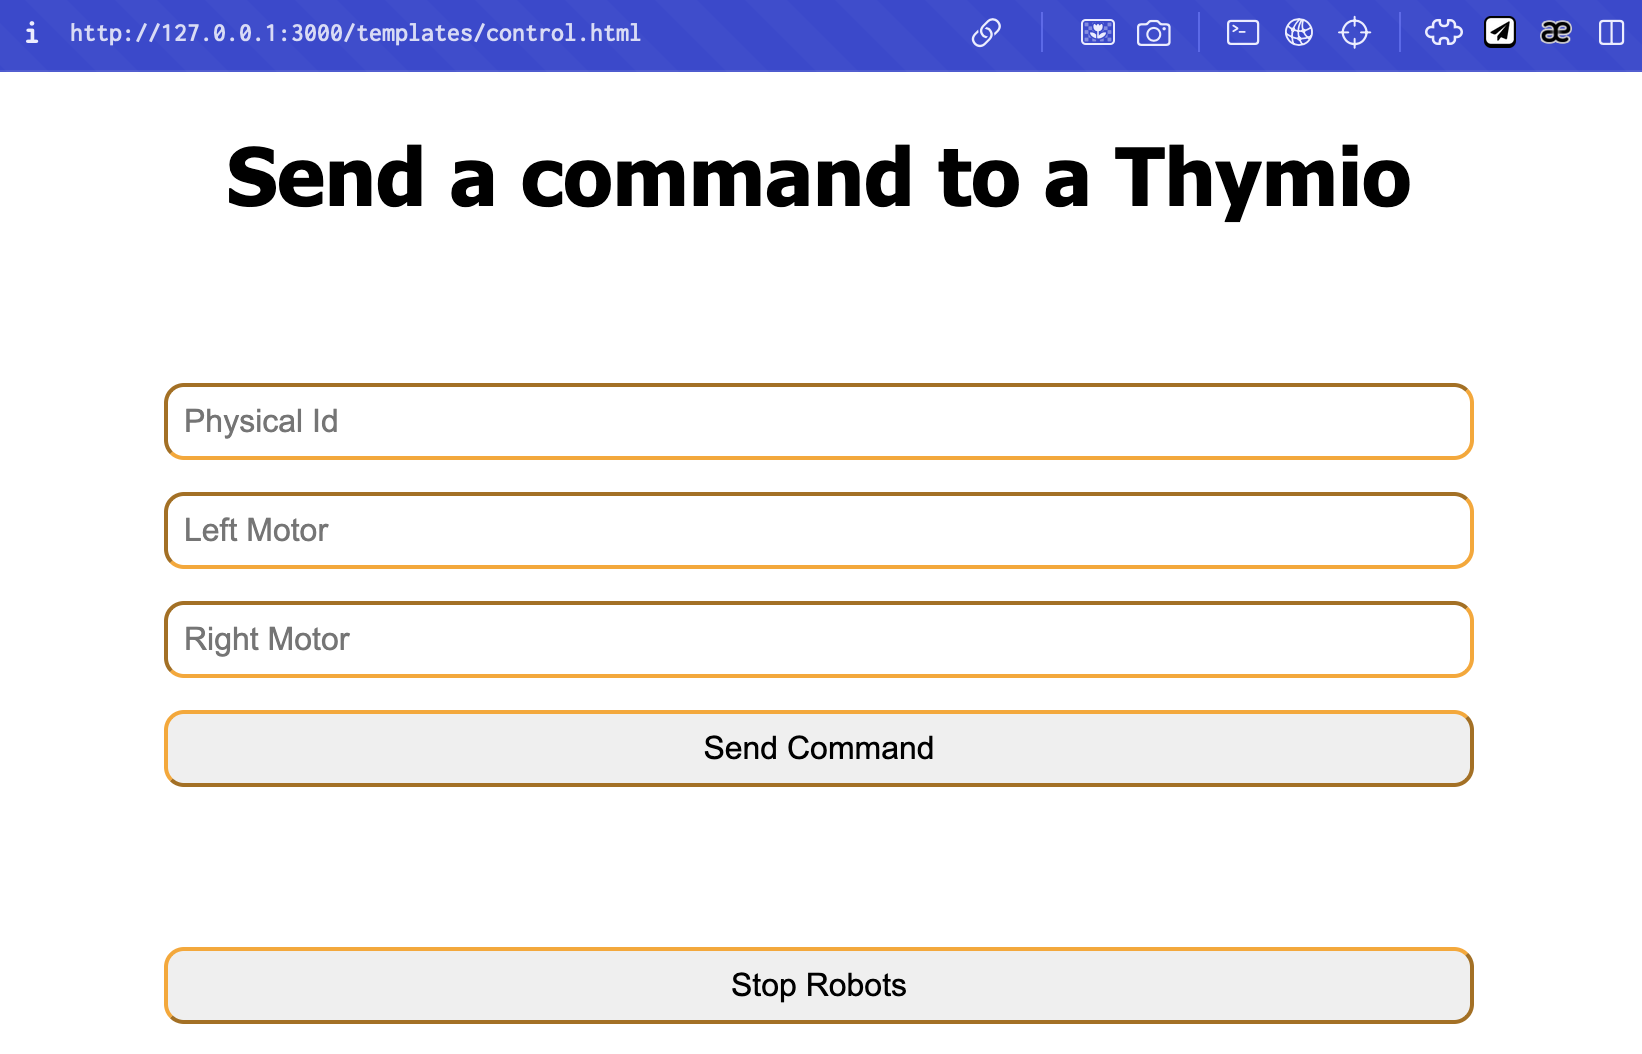
\includegraphics[width=.8\linewidth]{figures/web-interface.png}
    \caption{Interfaccia web per il controllo dei robot Thymio}
    \label{fig:web-interface}
\end{figure}

Lato programma aggregato, invece, troviamo l'implementazione di una classe che nasconde ogni tipo di dettaglio implementativo per il controllo dei robot, sia Wave che Thymio \cref{lst:robot-control}. Nel codice è presente solo l'implementazione di \verb|spinRight()| a fine dimostrativo ma gli altri comandi sono implementati in modo simile.

\lstinputlisting[language=Scala,label={lst:robot-control},caption={Classe per il controllo dei robot}]{listings/Robot.scala}

\section{Validazione}

Di seguito si riportano alcuni esempi di algoritmi aggregati applicati ai robot Wave e Thymio nello stesso ambiente per dimostrare che i requisiti sono stati soddisfatti mantenendo flessibilità, autonomia e eterogeneità del sistema.

\paragraph{Copia rotazione del Leader}
Programma Aggregato per far ruotare i robot del sistema seguendo la direzione del leader \cref{lst:rotate-leader} (figura \ref{fig:rotate-leader}).

\lstinputlisting[language=Scala,label={lst:rotate-leader},caption={Programma aggregato per far ruotare i robot del sistema seguendo la direzione del leader}]{listings/FollowLeaderRotating.scala}

\begin{figure}
    \centering
    \includegraphics[width=.99\linewidth]{figures/rotate-leader.pdf}
    \caption{Simulazione del programma aggregato per far ruotare i robot del sistema seguendo la direzione del leader .}
    \label{fig:rotate-leader}
\end{figure}

\paragraph{Formazione a ``linea''}
Programma aggregato che si occupa di allineare i robot del sistema al fine di creare una linea retta, si guardino le figure \ref{fig:line-shape-1} e \ref{fig:line-shape-2}. Il programma si occupa di scegliere un leader per definire il primo vertice della rette e posizionare i robot ad una certa distanza (crescente) dal leader in modo da formare una linea retta.

% \lstinputlisting[language=Scala,label={lst:line-shape},caption={Programma aggregato allineare i robot}]{listings/LineShape.scala}

\begin{figure}
    \centering
    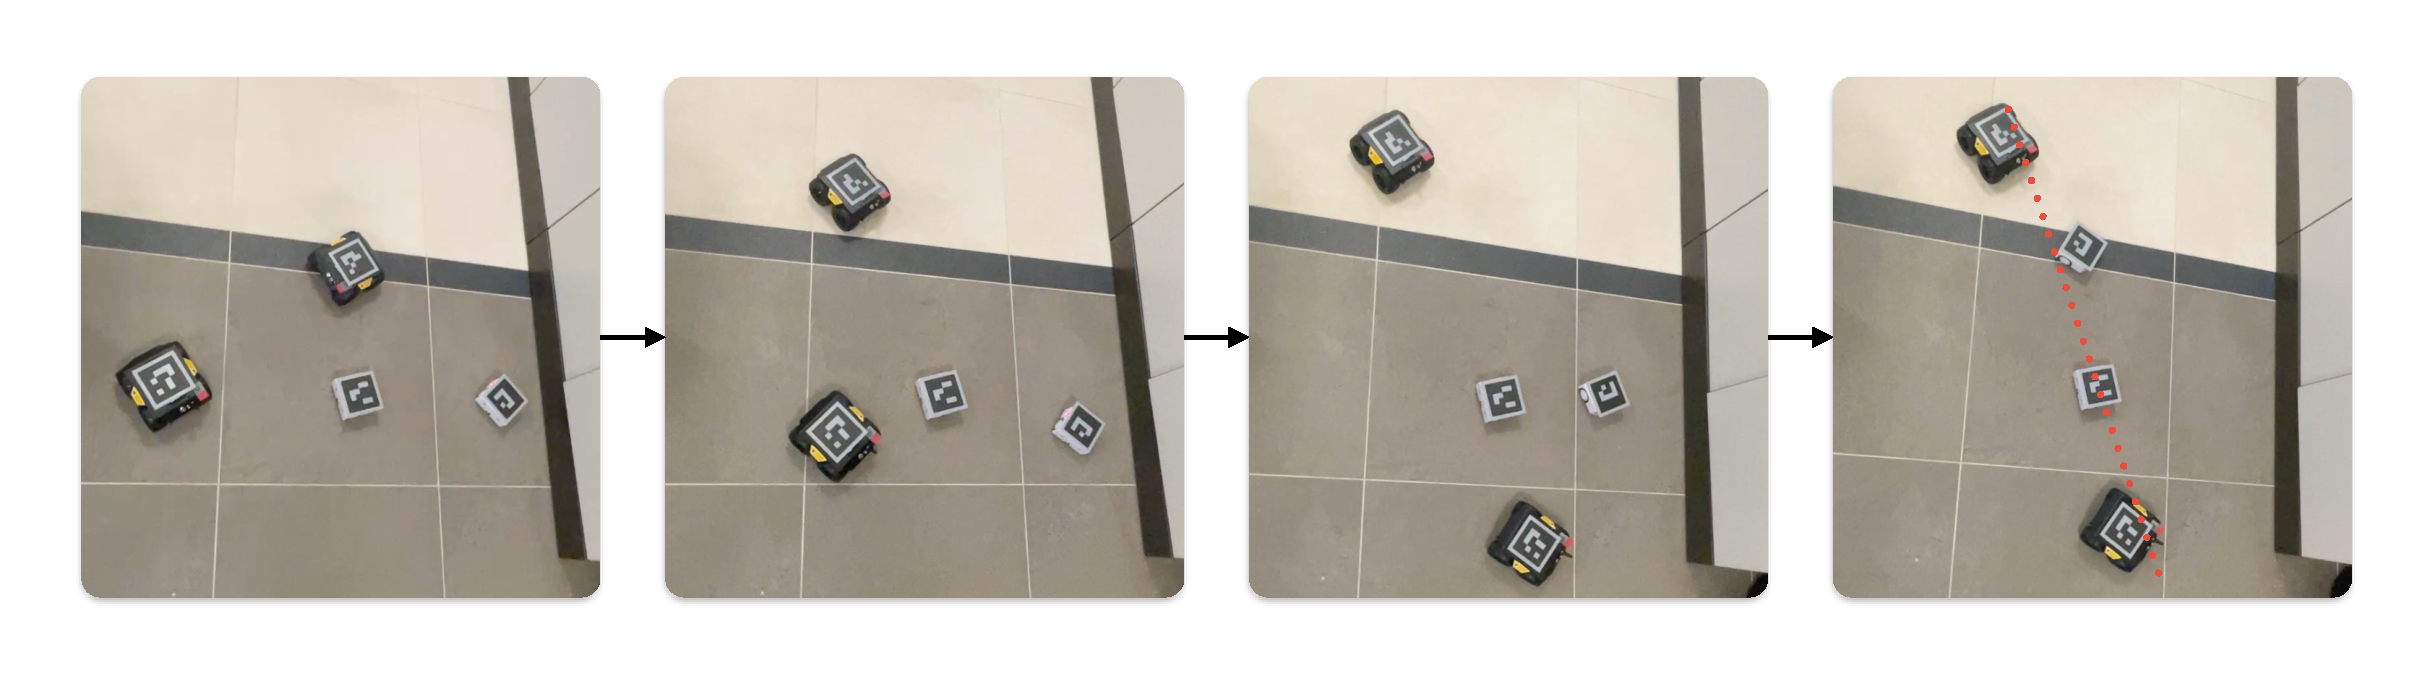
\includegraphics[width=.99\linewidth]{figures/line2.pdf}
    \caption{Simulazione del programma aggregato per allineare i robot.}
    \label{fig:line-shape-2}
\end{figure}

\begin{figure}
    \centering
    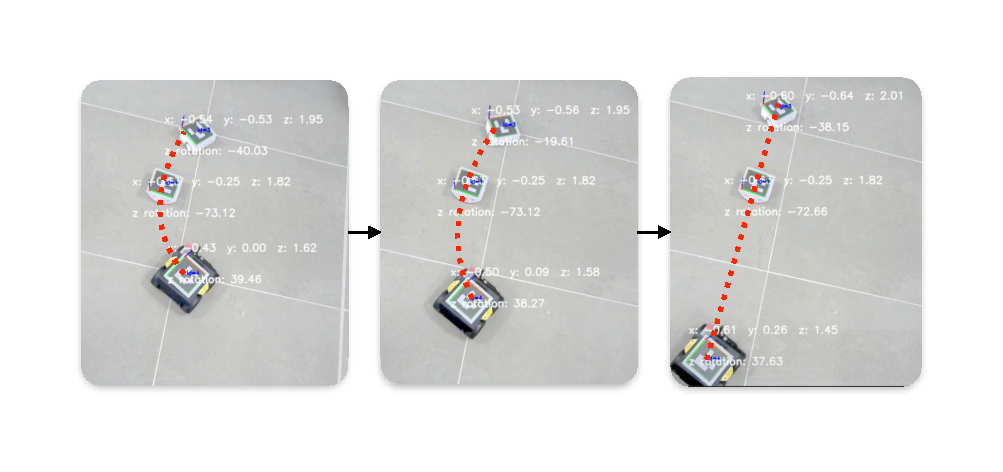
\includegraphics[width=.99\linewidth]{figures/line1.pdf}
    \caption{Simulazione del programma aggregato per allineare i robot dalla dalla visuale del programma di tracking dei Aruco Tag (la linea rossa è  stata inserita in post produzione).}
    \label{fig:line-shape-1}
\end{figure}

\paragraph{Formazione a ``cerchio''}

Programma aggregato che si occupa di definire un leader e produrre una formazione circolare intorno ad esso (codice \ref{lst:circle-shape}). È possibile notare dalla immagine \ref{fig:circle-formation} come il programma si comporti correttamente anche in situazioni anomale come la rimozione o l'inserimento di nuovo robot nell'ambiente.

\lstinputlisting[language=Scala,label={lst:circle-shape},caption={Programma aggregato allineare i robot}]{listings/CircleShape.scala}

\begin{figure}
    \centering
    \includegraphics[width=.99\linewidth]{figures/circle.pdf}
    \caption{Simulazione del programma aggregato per produrre un cerchio intorno ad un leader.}
    \label{fig:circle-formation}
\end{figure}

\section{File di configurazione}

Per gestire l'inserimento o la rimozione di nuovi robot nel sistema in modo dinamico si è scelto di utilizzare i file di configurazione nei \cref{lst:thymio-config} e \cref{lst:wave-config}.

Per la gestione dei file di configurazione all'interno del progetto Scala è stata utilizzata la libreria \textbf{uPickle}. È una libreria performante che permette un parsing veloce ed intuitivo, inoltre non ha problemi di dipendenze quindi può essere utilizzata in qualsiasi progetto Scala senza produrre conflitti \cite{uPickle}.

\lstinputlisting[language=Python, label={lst:thymio-config},caption={File di configurazione per i robot Thymio}]{listings/thymio-config.json}

\lstinputlisting[language=Python, label={lst:wave-config},caption={File di configurazione per i robot Wave}]{listings/wave-config.json}

Questi file di configurazione vengono caricati utilizzando la libreria uPickle \cite{uPickle}, si guardi \cref{lst:uPickle-read}.

\lstinputlisting[language=Scala,label={lst:uPickle-read},caption={Lettura dei file di configurazione}]{listings/upickle.scala}

%----------------------------------------------------------------------------------------
\chapter{Conclusione}
\label{chap:conclusione}

In questa tesi abbiamo dimostrato come sia possibile e semplice andare ad espandere il dominio, in funzione dell'integrazione di nuovi dispositivi robotici, del sistema che si si sta progettando utilizzando un sistema aggregato. La corretta integrazione, all'interno del orchestratore, del robot Thymio ha richiesto la sola implementazione di un'interfaccia sulla quale il sistema aggregato agisce per completare il ``round'' con la fase di ``act''. 
Nei lavori futuri si prevede una continua integrazione di nuovi robot e nuovi comportamenti che muovano l'insieme di robot in un ambiente caratterizzato da ostacoli.
%----------------------------------------------------------------------------------------

%----------------------------------------------------------------------------------------
% BIBLIOGRAPHY
%----------------------------------------------------------------------------------------

\backmatter

\bibliographystyle{alpha}
\bibliography{bibliography}

\begin{acknowledgements} % this is optional
Optional. Max 1 page.
\end{acknowledgements}

\end{document}
